%%%%%%%%%%%%%%%%%%%%%%%%%%%%%%%%%%%%%%%%%%%%%%%%%%%%%%%%%%%%%%%%%%%%%%%%%%%%%%%%
%
% \file       main.tex
% \brief      Главный файл настроек TeX проекта
% \date       24.08.22 - создан
% \author     Соболев А.А.
% \details    Для сборки в TexStudio - выбрать компилятор xelatex в настройках проекта
%             Для сборки при помощи CMake - mkdir build && cd build && cmake .. && make	
%
%%%%%%%%%%%%%%%%%%%%%%%%%%%%%%%%%%%%%%%%%%%%%%%%%%%%%%%%%%%%%%%%%%%%%%%%%%%%%%%%
\listfiles
\documentclass[headings=chapterprefix,a5paper]{book}
\usepackage[monochrome]{color}
\usepackage[12pt]{extsizes}
\usepackage[left=1.5cm,right=1.5cm,top=2.0cm,bottom=2.0cm]{geometry}
\linespread{1.0} % по умолчанию 1.0
%
\usepackage{tikz}
\usepackage{tocloft}
\usepackage{pgfornament}
\usepackage{amsmath}
\usepackage{gensymb} % Для знака градуса
\usepackage{cite}
\usepackage{pstricks}
\usepackage{psvectorian}
\usepackage{fontspec}
\usepackage{pdfpages}
\usepackage[russian]{babel}

\setmainfont[%
ItalicFont=NewCM10-Italic.otf,%
BoldFont=NewCM10-Bold.otf,%
BoldItalicFont=NewCM10-BoldItalic.otf,%
SmallCapsFeatures={Numbers=OldStyle}]{NewCM10-Regular.otf}

\setsansfont[%
ItalicFont=NewCMSans10-Oblique.otf,%
BoldFont=NewCMSans10-Bold.otf,%
BoldItalicFont=NewCMSans10-BoldOblique.otf,%
SmallCapsFeatures={Numbers=OldStyle}]{NewCMSans10-Regular.otf}

\setmonofont[ItalicFont=NewCMMono10-Italic.otf,%
BoldFont=NewCMMono10-Bold.otf,%
BoldItalicFont=NewCMMono10-BoldOblique.otf,%
SmallCapsFeatures={Numbers=OldStyle}]{NewCMMono10-Regular.otf}

\usepackage{afterpage}
%\usepackage[x-1a3]{pdfx} % Вызывает невозможность собирать в texstudio!
\usepackage{ctable}
\usepackage{longtable}
\usepackage{graphicx}
\graphicspath{ {./images/} }
%--------------------------------------
% эпиграф
\usepackage{epigraph}
\setlength{\epigraphwidth}{0.60\textwidth}%0.65
\renewcommand{\textflush}{flushleft} \renewcommand{\sourceflush}{flushleft}
\let\originalepigraph\epigraph 
\renewcommand\epigraph[2]{\originalepigraph{\textit{#1}}{\scriptsize{#2}}} %\textsc

%------------------------------------------------------------------------------------------------------------
%настройки для А4
%\usepackage[12pt]{extsizes}
%\usepackage[left=2.5cm,right=2.5cm,top=2.5cm,bottom=2.5cm]{geometry}
%\linespread{1.15} % по умолчанию 1.0
%------------------------------------------------------------------------------------------------------------
%настройки для А5
%\usepackage[11pt]{extsizes}
%\usepackage[left=1.5cm,right=1.5cm,top=2.0cm,bottom=2.0cm]{geometry}
%\linespread{1.0} % по умолчанию 1.0
%------------------------------------------------------------------------------------------------------------
%настройки для А4
%\newcommand{\corner}[1]{%
%	\begin{tikzpicture}[remember picture, overlay]
%	\node[anchor=north east, shift={(-2.5cm,-5.3cm)}] at (current page.north east){%
%		\pgfornament[width=2.2cm]{#1}};
%	\end{tikzpicture}%
%}
%------------------------------------------------------------------------------------------------------------
%настройки для А5
\newcommand{\corner}[1]{%
	\begin{tikzpicture}[remember picture, overlay]
	\node[anchor=north east, shift={(-1.5cm,-4.2cm)}] at (current page.north east){%
		\pgfornament[width=2.2cm]{#1}};
	\end{tikzpicture}%
}
%------------------------------------------------------------------------------------------------------------
\usepackage{indentfirst} % Первая строка главы - с красной строки
\setlength{\parindent}{1.0cm} % Отступ слева первой абзаца
\setlength{\parskip}{0.25cm} % Отступ между абзацами

% Заголовки сверху и снизу каждой страницы (Headers & footers)
\usepackage{fancyhdr}
\pagestyle{fancyplain}

\fancyhead[LE]{\fancyplain{}{}}
\fancyhead[CE]{\fancyplain{}{}}
\fancyhead[RE]{\fancyplain{}{}}

\fancyhead[LO]{\fancyplain{}{\bfseries\rightmark}}
\fancyhead[CO]{\fancyplain{}{}}
\fancyhead[RO]{\fancyplain{}{}}

\fancyfoot[LE]{\fancyplain{}{\bfseries\thepage}}
\fancyfoot[CE]{\fancyplain{}{}}
\fancyfoot[RE]{\fancyplain{}{\bfseries\scriptsize \MyVarBookName}}

\fancyfoot[LO]{\fancyplain{}{\bfseries\scriptsize \MyVarAuthorName }}
\fancyfoot[CO]{\fancyplain{}{}}
\fancyfoot[RO]{\fancyplain{}{\bfseries\thepage}}

\renewcommand{\footrulewidth}{0.4pt}
\renewcommand{\chaptermark}[1]{%
	\markboth{#1}{}%
}

\renewcommand{\chaptermark}[1]{\markright{\chaptername\ \thechapter.\ #1}{}}

% Пустая страница
\newcommand\blankpage{%
	\null
	\thispagestyle{empty}
	\newpage
}

\newcommand{\sdash}{\nobreakdash-}  % Дефис неразрывный без пробелов до и после
\newcommand{\ndash}{\nobreakdash~--~}  % Короткое тире неразрывное с пробелами до и после
\newcommand{\mdash}{\nobreakdash~---~} % Длинное тире неразрывное с пробелами до и после

\renewcommand{\cftchappresnum}{Глава }
\setlength{\cftbeforechapskip}{0.7em}
%\renewcommand\cftchapafterpnum{\vskip 0em} % for spacing after each entry
\AtBeginDocument{\addtolength\cftchapnumwidth{\widthof{\bfseries Глава~ }}}

\renewcommand\cftchapdotsep{\cftdotsep} % Добавление точечек к элементу chapter

\newcommand\MyVarAuthorName{А.А.~Соболев}
\newcommand\MyVarBookName{Повесть о сплаве на байдарке}
\newcommand\MyVarBookNamesec{по рекам Лидь, Чагода, Чагодоща}

\newcommand{\UDK}{821.161.1}
\newcommand{\BBK}{84 (2Рос-Рус) 6}
\newcommand{\BibCode}{C54}
\newcommand{\ISBN}{ISBN 978-5-6048796-4-1}

\renewcommand*{\thefootnote}{\fnsymbol{footnote}}
\usepackage[symbol]{footmisc}

\newcommand{\vepsianrose}{%
	\begin{figure}[h!]
%		\vspace*{-77mm}
		\vspace*{-70mm}
%		\hspace*{8.15cm}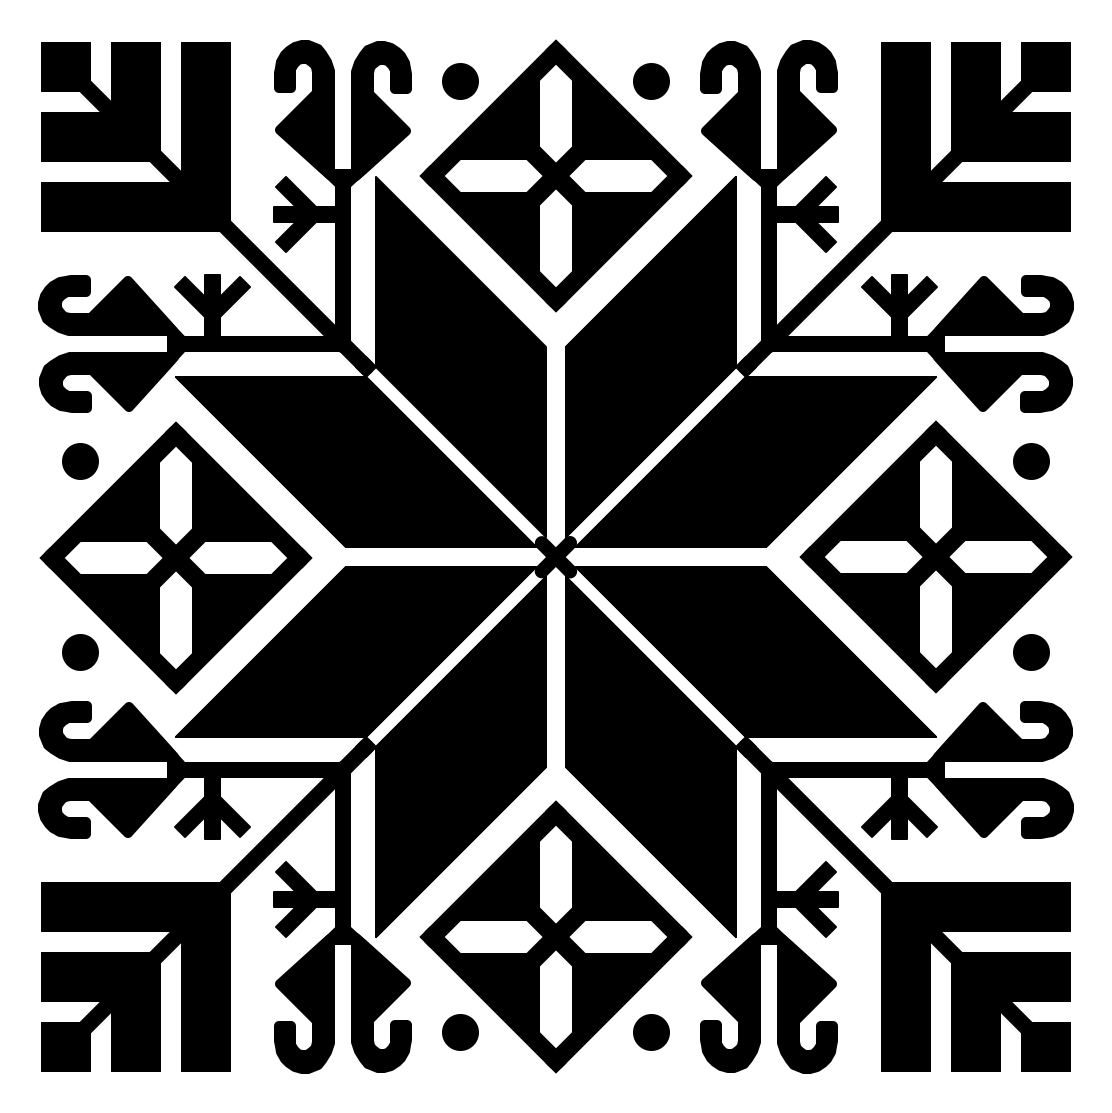
\includegraphics[scale=0.1]{vepsroseb} % Черный
		\hspace*{8.8cm}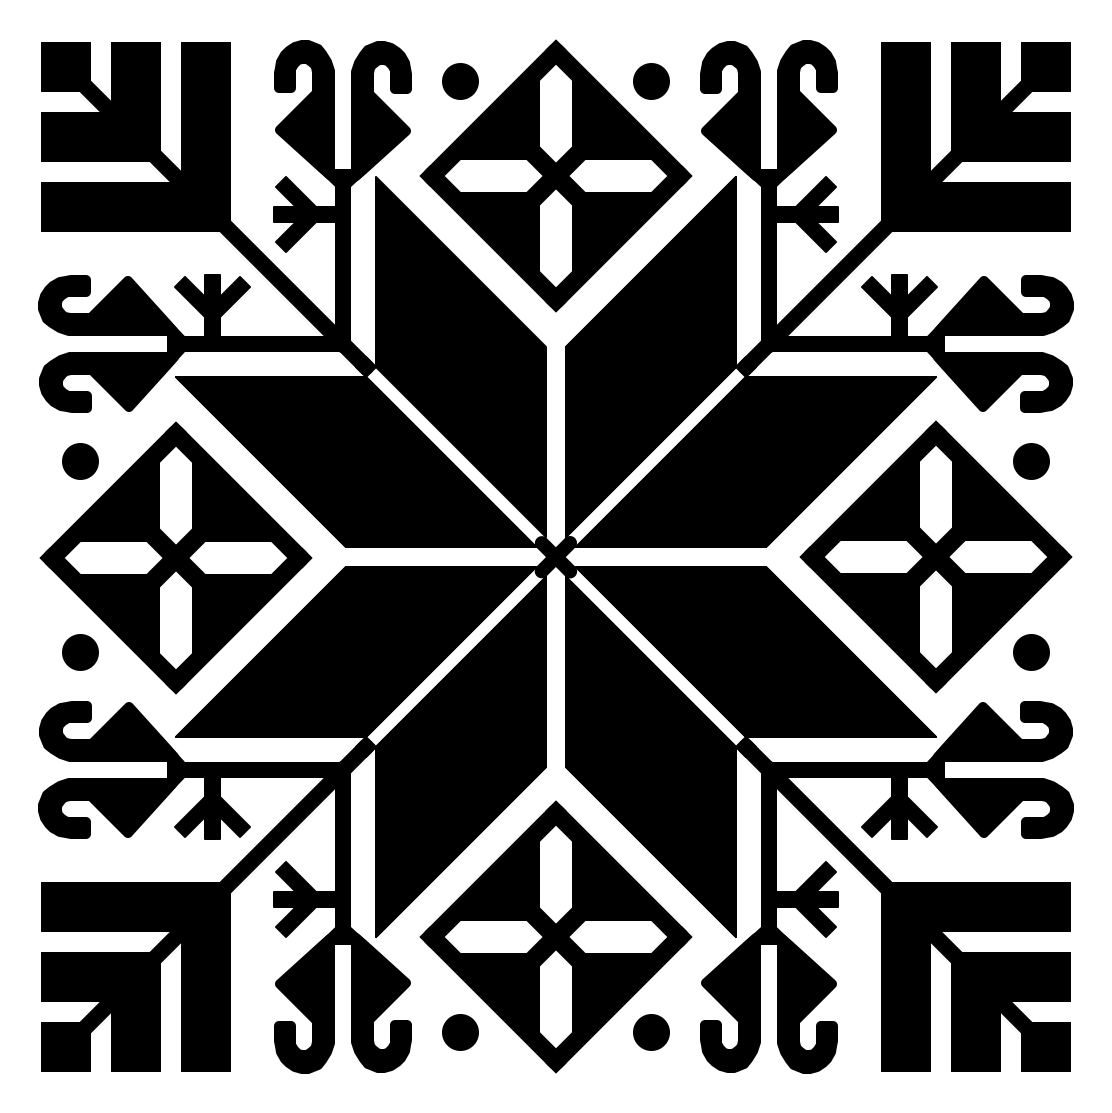
\includegraphics[scale=0.1]{vepsroseb} % Черный
	\end{figure}
	\vspace*{4.0cm}
}

\usepackage{titlesec}
\usepackage[colorlinks=true,linktoc=all]{hyperref} % hyperfootnotes=false - не выделять сноски
\usepackage{bookmark}

\begin{document}
%%%%%%%%%%%%%%%%%%%%%%%%%%%%%%%%%%%%%%%%%%%%%%%%%%%%%%%%%%%%%%%%%%%%%%%%%%%%%%%%
%
% Координаты стоянок
%
%%%%%%%%%%%%%%%%%%%%%%%%%%%%%%%%%%%%%%%%%%%%%%%%%%%%%%%%%%%%%%%%%%%%%%%%%%%%%%%%
% р.Лидь
\newcommand\CoordsLidSeventeenStapel{${N~59.77112\degree~E~34.87456\degree}$} % Стапель 2017 г.
\newcommand\CoordsLidSeventeenFirst{${N~59.68915\degree~E~34.89413\degree}$} % 1 стоянка 2017 г.
\newcommand\CoordsLidSeventeenTresno{${N~59.68745\degree~E~34.92153\degree}$} % Тресновская ГЭС 2017 г.
\newcommand\CoordsLidSeventeenTruba{${N~59.67229\degree~E~34.94233\degree}$} % Труба-мост 2017 г.
\newcommand\CoordsLidSeventeenSeloLid{${N~59.64044\degree~E~35.06237\degree}$} % Ночёвка около с.Лидь 2017 г.
\newcommand\CoordsLidSeventeenNearZaborie{${N~59.53621\degree~E~35.19714\degree}$} % Ночёвка около Заборья 2017 г.
\newcommand\CoordsLidFifteenStapel{${N~59.51290\degree~E~35.21290\degree}$} % Стапель 2015 г.
\newcommand\CoordsLidFifteenGrishkino{${N~59.46437\degree~E~35.17958\degree}$} % 1 стоянка 2015 г.
\newcommand\CoordsLidRightProtoka{${N~59.42453\degree~E~35.15822\degree}$} % Проход в правой протоке 2017 г.
\newcommand\CoordsLidSeventeenDnevka{${N~59.42332\degree~E~35.15214\degree}$} % Днёвка 2017 г.
\newcommand\CoordsLidSuperPlace{${N~59.38460\degree~E~35.17379\degree}$} % Супер-место
\newcommand\CoordsLidFifteenTurgosch{${N~59.32765\degree~E~35.17302\degree}$} % Ночёвка около Тургощи, 2015 г.
\newcommand\CoordsLidSeventeenBeforeLast{${N~59.19729\degree~E~35.17220\degree}$} % Ночёвка предпоследняя, 2017 г.
%%%%%%%%%%%%%%%%%%%%%%%%%%%%%%%%%%%%%%%%%%%%%%%%%%%%%%%%%%%%%%%%%%%%%%%%%%%%%%%%
% р.Горюн
\newcommand\CoordsGorunSixteenStapel{${N~59.29726\degree~E~34.92587\degree}$} % Стапель 2016 г.
\newcommand\CoordsGorunSixteenPlotina{${N~59.27053\degree~E~34.91910\degree}$} % Плотина 2016 г.
\newcommand\CoordsGorunSixteenUstie{${N~59.21645\degree~E~34.92776\degree}$} % Устье Горюна 2016 г.
%%%%%%%%%%%%%%%%%%%%%%%%%%%%%%%%%%%%%%%%%%%%%%%%%%%%%%%%%%%%%%%%%%%%%%%%%%%%%%%%
% р.Чагода
\newcommand\CoordsChagodaSixteenFirst{${N~59.21645\degree~E~34.92776\degree}$} % 1 стоянка 2016 г.
\newcommand\CoordsChagodaGood{${N~59.21520\degree~E~34.95573\degree}$} % Хорошее место
\newcommand\CoordsChagodaFifteenFirstDnevka{${N~59.15709\degree~E~35.23621\degree}$} % 1-ая днёвка 2015 г.
\newcommand\CoordsChagodaSixteenDrunk{${N~59.15804\degree~E~35.24190\degree}$} % Пьянка 2016 г.
%%%%%%%%%%%%%%%%%%%%%%%%%%%%%%%%%%%%%%%%%%%%%%%%%%%%%%%%%%%%%%%%%%%%%%%%%%%%%%%%
% р.Чагодоща
\newcommand\CoordsChagodoschaSemaphor{${N~59.15379\degree~E~35.30460\degree}$} % Семафор
\newcommand\CoordsChagodoschaFifteenGoToStore{${N~59.15912\degree~E~35.32931\degree}$} % Высадка в магазин 2015 г.
\newcommand\CoordsChagodoschaSixteenGoToStore{${N~59.15858\degree~E~35.32970\degree}$} % Высадка в магазин 2016 г. антистапель 2017~г, 2018~г.
\newcommand\CoordsChagodoschaNineteenStapel{${N~59.16139\degree~E~35.37266\degree}$} % Cтапель, л.б., 2019~г.
\newcommand\CoordsChagodoschaMegrino{${N~59.13567\degree~E~35.61832\degree}$} % Ночёвка за Мегрино, л.б., 2015, 2016, 2019 гг.
\newcommand\CoordsChagodoschaNineteenSecond{${N~59.06962\degree~E~35.86246\degree}$} % 2 ночёвка, л.б., 2019 г.
\newcommand\CoordsChagodoschaFifteenKaban{${N~59.08257\degree~E~35.94123\degree}$} % Ночёвка c кабанами 2015 г.
\newcommand\CoordsChagodoschaSixteenNearKaban{${N~59.08569\degree~E~35.94522\degree}$} % Ночёвка около кабанов 2016 г.
\newcommand\CoordsChagodoschaNineteenDnevka{${N~59.12318\degree~E~36.03306\degree}$} % Днёвка 2019 г.
\newcommand\CoordsChagodoschaFifteenSecondDnevka{${N~59.18169\degree~E~36.11501\degree}$} % 2-ая днёвка 2015 г.
\newcommand\CoordsChagodoschaSixteenEmergencyNignt{${N~59.19177\degree~E~36.15595\degree}$} % Экстренная ночёвка 2016 г.
\newcommand\CoordsChagodoschaZagrivieParom{${N~59.18664\degree~E~36.22300\degree}$} % Паром в Загривье 2015 2016 гг.
\newcommand\CoordsChagodoschaFifteenAntistapel{${N~59.19248\degree~E~36.23246\degree}$} % Антистапель 2015 г.
\newcommand\CoordsChagodoschaSixteenDnevka{${N~59.16482\degree~E~36.28046\degree}$} % Днёвка 2016 г.
\newcommand\CoordsChagodoschaNineteenBeforeLast{${N~59.15593\degree~E~36.32325\degree}$} % Ночёвка, л.б., 2019~г.
\newcommand\CoordsChagodoschaNineteenAntistapel{${N~59.05216\degree~E~36.40635\degree}$} % Антистапель л.б., 2019~г.
\newcommand\CoordsChagodoschaSixteenSalin{${N~58.99856\degree~E~36.52885\degree}$} % Последняя ночёвка в урочище Салынь, 2016 г.
\newcommand\CoordsChagodoschaSixteenAntistapel{${N~58.97235\degree~E~36.58830\degree}$} % Антистапель, 2016 г.
%%%%%%%%%%%%%%%%%%%%%%%%%%%%%%%%%%%%%%%%%%%%%%%%%%%%%%%%%%%%%%%%%%%%%%%%%%%%%%%%
% р.Песь
\newcommand\CoordsPesEighteenStapel{${N~58.93065\degree~E~34.15118\degree}$} % Cтапель, 2018 г.
\newcommand\CoordsPesZavalFirstBezObnosa{${N~58.92815\degree~E~34.20071\degree}$} % Завал без обноса
\newcommand\CoordsPesEighteenFirst{${N~58.92943\degree~E~34.23585\degree}$} % 1 ночёвка
\newcommand\CoordsPesZavalSecondWithObnos{${N~58.92517\degree~E~34.27858\degree}$} % Завал с обносом
\newcommand\CoordsPesEighteenBeforeYahnovo{${N~58.89480\degree~E~34.35690\degree}$} % Ночёвка перед Яхново
\newcommand\CoordsPesEighteenAfterMyakishevo{${N~58.84678\degree~E~34.44593\degree}$} % Ночёвка после Мякишево
\newcommand\CoordsPesEighteenDnevka{${N~58.90267\degree~E~34.60336\degree}$} % Днёвка 2018 г.
\newcommand\CoordsPesEighteenAfterMinci{${N~58.96410\degree~E~34.84470\degree}$} % Ночёвка после Минцов
\newcommand\CoordsPesZavalThirdBezObnosa{${N~58.94978\degree~E~34.87727\degree}$} % Завал без обноса
\newcommand\CoordsPesZavalFourthWithObnosGRAND{${N~58.93968\degree~E~34.88977\degree}$} % ГРАНД-Завал c обносом
\newcommand\CoordsPesEighteenKrutik{${N~58.96258\degree~E~35.12499\degree}$} % Ночёвка в устье Крутика
\newcommand\CoordsPesEighteenLast{${N~59.02471\degree~E~35.21774\degree}$} % Последня ночёвка
%%%%%%%%%%%%%%%%%%%%%%%%%%%%%%%%%%%%%%%%%%%%%%%%%%%%%%%%%%%%%%%%%%%%%%%%%%%%%%%%
\relpenalty=10000
\binoppenalty=10000
\clubpenalty=10000  % Это костыль против
\widowpenalty=10000 % "висячих" строк

\righthyphenmin=200 % Избавляемся
{\sloppy
\includepdf{обложка_а5.pdf}
\newpage
\null
\thispagestyle{empty}
\newpage
\begin{titlepage}
	\newpage
	\begin{center}
		\huge \textbf \MyVarAuthorName
	\end{center}	
	\vspace{3cm}	
	
	\begin{center}
	\begin{tikzpicture}
	\fill[fill=black!30!green,] (0,0) rectangle (10.8,0.2);
	\end{tikzpicture}
	\end{center}
	
	\begin{center}
		\huge \textbf {ПОВЕСТЬ О СПЛАВЕ\\НА БАЙДАРКЕ}
	\end{center}	
	\vspace{0.0cm}

	\begin{center}
	\begin{tikzpicture}
	\fill[fill=black!30!green,] (0,0) rectangle (10.8,0.2);
	\end{tikzpicture}
	\end{center}

	\begin{center}
		\LARGE {по рекам Лидь, Чагода, Чагодоща}
	\end{center}

	\begin{center}
	\begin{tikzpicture}
	\fill[fill=black!30!green,] (0,0) rectangle (10.8,0.2);
	\end{tikzpicture}
	\end{center}
		
	\vspace{\fill}	
	\begin{center}
		\normalsize
		Москва \linebreak 
		2022 \linebreak
		Самиздат
	\end{center}	
\end{titlepage}

%\chapter*{}
%\newpage
{
\thispagestyle{empty}
%
\small{
\begin{flushleft}
\textbf{%
	УДК\UDK \\
	ББК\BBK \\
	\BibCode \\
}
\end{flushleft}
%
\vspace{3cm}
%
\begin{flushright}
{
\begin{tabular}[c]{>{\raggedright}m{14mm} >{\raggedright}m{95mm} }
	\textbf{\BibCode} & \MyVarAuthorName \tabularnewline
	~ & \MyVarBookName \tabularnewline
	~ & \MyVarBookNamesec \tabularnewline
	~ & М.:~ООО~<<ИПЦ~"`Маска"'>> ,~2022\mdash 128 c. \tabularnewline
	~ & \textbf{\ISBN}
\end{tabular}
}
\end{flushright}
%
\vspace{4.0cm}
%
\begin{flushright}
\textbf{%
	УДК\UDK \\
	ББК\BBK \\
	\BibCode \\
}
\end{flushright}
%
%\vspace{\fill}
\vspace{1.0cm}
%
}
{
\begin{longtable}[c]{>{\raggedright}m{55mm} >{\raggedleft}m{55mm} }
	\textbf{\ISBN} & {\copyright~\MyVarAuthorName,~2022} \tabularnewline
\end{longtable}
}
}
%\afterpage{\blankpage}
\chapter*{}

В повести рассказывается о первом длительном самостоятельном сплаве автора одной байдаркой по маршруту \textnumero57 на границе Ленинградской и Вологодской областей. Даётся развёрнутое описание каждого дня похода с личными ощущениями и переживаниями руководителя, оказавшегося на реке с двумя малознакомыми матросами. На долю путешественников выпадают испытания, которые придётся преодолеть вдали от цивилизации один на один с природой, и с этой задачей они успешно справятся. Также вашему вниманию предлагается предыстория этого похода и множество отвлечённых рассуждений.

\vspace{\fill}
\begin{flushright}
	\copyright~Соболев~А.А.~2022
\end{flushright}
%\afterpage{\blankpage}
% Замена \blankpage в данном случае:
\newpage
\null
\thispagestyle{empty}
\newpage
%
{
%\setlength{\cftbeforetoctitleskip}{1.5cm}%чтобы влезло на 1 страницу 11 шрифт - 15 глав
%\setlength{\cftbeforetoctitleskip}{0.5cm}%чтобы влезло на 1 страницу 12 шрифт - 15 глав
%\setlength{\cftbeforetoctitleskip}{-0.5cm}%чтобы влезло на 1 страницу 12 шрифт - 15 глав + Литература
\setlength{\cftbeforetoctitleskip}{-0.1cm}%чтобы влезло на 1 страницу 12 шрифт - 15 глав + Литература + Слово "Глава"
\pdfbookmark[0]{\contentsname}{toc} % Добавлять перед \tableofcontents
\tableofcontents
}
\afterpage{\blankpage}
\chapter*{}
\begin{flushright}
\vspace{2.0cm}
\textit{ \large {
Жаждущим диких походов посвящается.\\
\vspace{\fill}
Все имена, названия, события,\\
время и место действия вымышлены,\\
а совпадения случайны.
}}
\end{flushright}



\afterpage{\blankpage}
%
\chapter{Несколько слов о сплавах} 
\corner{64}

\epigraph{%Не нужен бродягам дом и уют \\
%	Нужны - Океан, Земля \\
%	Что звёзды Медведицы им поют \\
%	Не знаем ни ты, ни я \\
%	~...\\
	~\\
	~\\	
	~\\	
	Вел\'{и}к Океан и Земля велик\'{а} \\
	Надо бы всё пройти \\
	Большая Медведица издалека \\
	Желает тебе пути}
	{
	\begin{flushright}
		\small{Станислав~Пожлаков,\\<<Баллада~о~детях~Большой~Медведицы>> из~х/ф~<<Идущие~за~горизонт>>,~1972}%\\(экранизация~повести~Олега~Куваева\\ <<Птица~капитана~Росса>>,~1968)
	\end{flushright}
	}

Неизвестно, от чего получаешь б\'{о}льшее удовольствие\mdash от подготовки к сплаву, от собственно самого сплава или от смакования воспоминаний о нём в кругу друзей, родственников и единомышленников. Каждая часть этого действа хороша по\sdash своему и от каждой остается определённый отпечаток, который уже никогда никуда не денется и будет греть душу туриста\sdash водника долгими зимними вечерами.

У Феликса Квадригина в его книге <<На байдарке>> есть строки о том, что водниками не становятся\mdash в водный туризм втягивают. И это действительно так. Правда, осознаётся это только после нескольких сплавов. Меня втянула в водный туризм тогда ещё будущая жена, предложив сходить в сплав, сама видимо не вполне осознавая, на что идёт. С тех пор в моей душе поселился огонёк странствий по водным просторам нашей необъятной Родины.

Первый сплав\mdash это всегда особенное действо. После него люди либо брезгливо убегают прочь от <<этих ненормальных>> с рюкзаками и вёслами, так и не поняв, зачем всё это надо, либо в их сердцах поселяется огонь странствий, а в мозгу заседает заноза, не дающая покоя ровно от предыдущего сплава до следующего. 

С первым сплавом мне и будущей жене повезло\mdash мы попали на Южный Урал, реку Зил\'{и}м. Сплавлялись около 10 дней, на катамаранах, вместе с огромной компанией в 50 человек, среди которых было 5 или даже больше инструкторов. Река Зилим летом спокойная, но мелковатая в верховьях. Туристы-водники, любящие бурлящую воду и белую пену, брезгливо называют такие сплавы матрасными. Что ж, это в какой-то мере справедливо\mdash течение реки спокойное, грести особо не надо, лишь местами могут встретиться быстринки и подобия перекатов. Но, в конце концов, все виды отдыха хороши. Мне, жене, да и всем тем людям, с кем мы ходили, нравится именно такой вид сплава\mdash без риска для жизни, но со спокойным единением с необычайно красивой природой нашей страны, когда забываешь обо всех проблемах и заботах, тяготящих тебя в обычной жизни\ldots

Инструкторы были заняты на стоянках приготовлением еды на костре, заготовкой дров бензопилами, ну и конечно травлей анекдотов. Фактически, нам, как новичкам, оставалось только поставить палатку, покидать в неё свои вещи, да наслаждаться жизнью, травить байки и ожидать пока поспеет вкуснейшая вечерняя похлёбка от штатного кока, да закипит чай с душистыми травами, собранными на местных лугах. 

Нам с будущей женой всё было в новинку\mdash мы никогда не ходили в походы или сплавы. И хотя я много раз порывался выбраться в какой-нибудь поход, каждый раз меня что\sdash то останавливало. Причём перспектива походной жизни меня никогда не страшила\mdash наоборот, мне очень хотелось попасть в настоящий поход и приобщиться к дикому туризму, но всё почему-то не получалось. А тут мы удачно попали в большую команду, нам выдали палатку, снаряжение. Словом, мы упростили себе <<порог вхождения>> в дикий туризм тем, что вопросы, связанные с маршрутом, заброской и выброской, снаряжением решали не мы, а руководители.

В первом сплаве мы испытали на себе и каменистые отмели, когда острые камни противно трутся о дно катамарана, и быстрые перекаты, когда река ускоряется в скалах Южного Урала и надо активно подгребать веслом, выправляя курс. Было и жаркое палящее солнце, моментально высушивающее намокшую одежду, и ураганный ветер с дождём, порой настигающим совсем не вовремя\mdash на воде или когда ставишь палатку. Была и походная баня. Это изобретение заслуживает отдельного рассказа, а тот, кто её придумал, безусловно, достоин какой-нибудь премии.

Баня в походе\mdash это Баня с Большой Буквы. Помыться, в принципе, можно и в реке, но разве это хоть в какой\sdash то мере сравнится с ощущениями от Бани? Распаренный, вдыхая аромат трав, подстеленных на каменистый берег в роли коврика, хлещешь себя берёзовым, дубовым, еловым, пихтовым веником\mdash любым каким смог сделать. Инструктор, который уже тебе товарищ и друг и с которым выпиваешь по чарке за ужином, обсуждая как классно вообще жить на Земле, плещет воды на каменную печь и по Бане расходится превосходный пар, обдавая тело волнами колкого тепла. Веники ходят по спинам, раскаляя их докрасна\ldots~После, Баня открывается и распаренные, будто заново родившиеся, счастливые туристы с визгами восторга бегом мчатся в речку\mdash окунуться с головой, остудиться и проплыть пару метров, а потом обратно\mdash греться и снова париться. Особого шика добавляет то, что если во время этого действа идёт тёплый летний дождик\ldots  

Сама Баня состоит собственно из печки и палатки, которую ставят потом поверх протопленной печи. Печь складывают из камней, коих имеется неограниченное количество на берегах рек Южного Урала, выбирая при этом такие, чтобы не трескались при нагреве. Как выбирать\mdash эту науку постигли только Инструкторы, ходящие на эти реки как к себе домой по несколько раз каждый год. Потом ставится палатка\mdash вроде торговой, представляющая из себя куб или прямоугольный параллелепипед и сверху накрывается дополнительно полиэтиленовой пленкой, чтобы меньше уходило тепло и пар. Далее кто-нибудь снаряжается за травой или папоротником для банного пола и ветками для веников. Всё, потрясающие ощущения гарантированы!

После Бани чистые, обновленные туристы усаживаются к импровизированному столу вкушать отменный ужин от кока и пить вкуснейший чай с местными травами. Уже начинает темнеть и сытые, чистые, счастливые люди разбредаются кто куда\mdash часть попеть у костра, часть медитировать на берег реки, кто-то подальше от костра и людей смотреть или фотографировать звёзды, а кто по палаткам творить походную романтику. Уверен, что походная романтика создала немало счастливых семей, где Она знает, что Он может добыть дров и развести огонь и вообще, что топор из рук не валится. Он, в свою очередь, знает, что Она может фактически из ничего приготовить вкуснятину к ужину и уж конечно оба они\mdash туристы-водники, всегда готовые прийти на помощь друг другу и поделиться последним, неважно, куском хлеба или сухим спальником. 

Стапель на Зилиме был в Толп\'{а}рово, а с снимались с маршрута в Именд\'{я}шево. Толпарово\mdash прекрасное место! Мост через реку, поросшие соснами склоны горы Карамал\'{ы}, сельские домики, сельхозтехника, огороженные пастбища, стога сена\ldots~Я смотрел на всю эту красоту и не мог поверить, что всё происходящее\mdash реальность. Мне казалось это какой\sdash то параллельный мир. Какая\sdash то вдруг Швейцария, внезапно. Но нет, это наша страна, это Южный Урал! Всё\sdash таки как велика, необъятна, красива наша Родина!

На маршруте мы побывали около небольшого интересного озера недалеко от берега реки. Вода в нём была прозрачной, небесно\sdash голубого цвета, и очень\sdash очень холодной. Погода в тот момент была прохладной и дождливой, но всё равно среди нашей команды нашлись смельчаки, окунувшиеся в это природное чудо. Потом мы побывали в пещере Победа, для чего потребовалось карабкаться вверх в горы по крутым склонам – вход в пещеру находился высоко наверху. Всё это, конечно же, оставило неизгладимые впечатления в наших сердцах! Попасть в такое приключение было настоящей удачей.

Так я изложил общие впечатления человека, втянутого по собственной воле в туристическое братство и в первом же сплаве произнёсшего страшную клятву туристов-водников. После первого сплава был и второй\mdash по Башкирской реке Белая (Агид\'{е}ль) компанией из 10 человек. Этот, более камерный что ли, сплав на катамаранах также нам очень понравился. В перерыве между первым и вторым сплавом моя женщина, спутница\sdash красавица, окончательно и бесповоротно стала моей спутницей жизни, что ещё раз подтверждает вышесказанное про походную романтику. Так что второй раз на воду мы встали уже будучи супругами.

Сплав по Белой, безусловно, отличался от предыдущего\mdash хотя бы впятеро меньшим количеством народа. У нас также были переходы и днёвки, походные Бани и созерцание звёзд, дегустация мёда и медовухи с местной пасеки, рыбалка и фотоохота. Ещё было посещение пещеры Сказка, расположенной на живописнейшем склоне горы около Акбул\'{а}тово, и К\'{а}повой пещеры (пещера Шульг\'{а}н\sdash Таш), в которой раньше жили доисторические люди. Впечатлений также хватало, мы набирались опыта\mdash благо есть у кого\mdash наши руководители на всех реках Южного Урала были как родные.

Эти два сплава заложили, можно сказать, основу будущим моим путешествиям. В них я понял, что даже такой не слишком подготовленный человек, как я, вполне справляется с походным бытом и что никаких особенных премудростей не требуется. Нужно лишь желание и стремление идти вперед. Из этих сплавов я вынес очень хорошие уроки организации всего этого действа, приобрёл уверенность в силе человека противостоять природе и непогоде. А~это ли не главное? Где\sdash то в глубине души загорелась мысль, что я, в принципе, мог бы и сам организовать такое мероприятие, как сплав.

\begin{center}
	\psvectorian[scale=0.4]{88} % Красивый вензелёк :)
\end{center}

\chapter{Байдарка}
\corner{64}

После второго сплава был большой перерыв. Не~удавалось выкроить время, чтобы попасть на~Южный Урал, да и, откровенно говоря, хотелось чего\sdash то нового. Правда,~пока сам не понимал чего. Потом, вместе с~рассказами начальника о байдарочных сплавах, пришло осознание\mdash вот оно, это новое! Это~же~то, что надо! Байдарка! Отдельный корабль! Твой! Собственный! Никаких~инструкторов, всё делать самому! Тебе~никто не~указ! Ты\mdash бесстрашный рекоплаватель и~первооткрыватель! Ты\mdash Капитан корабля! Сердце моё застучало чаще, разум затуманился. 

После того, как туман развеялся, было много разговоров и рассказов начальника о том, что такое байдарочный сплав и с чем его едят. Вместе с разговорами пришло и второе осознание\mdash идём на реку! Рассуждали о том, на какую реку идти, как забрасываться и как сниматься с маршрута\ldots~а кроме того\mdash нужны были байдарки. Мой выбор пал на консервативную <<Таймень>>, поскольку нашлись ещё школьные знакомые-одноклассники, готовые отдать каркас, или как говорят водники, <<кости>>, ну а новую ПВХ оболочку, <<шкуру>>, купить не проблема. Не обошлось без влияния наших разговоров\mdash начальник рассказывал, что места в <<Таймени>> просто завались и это действительно оказалось так.

Вообще, тут стоит отметить, байдарочный поход в~данном случае оказался неизбежен, как крах мирового капитализма. Я~попал на работу в <<почтовый ящик>>, начальник, увлекающийся водным туризмом, сама атмосфера <<почтового ящика>>\ldots~всё это настолько тонко, что почти непередаваемо людям, которым никогда не~пришлось столкнуться с этим. А когда я поделился с~начальником рассказами о своих прошлых сплавах, то тут\sdash то, надо полагать, в его голове и сложилась картина вновь замаячившей возможности оказаться в привычной стихии. Постепенно мы оба свыклись с мыслью, что однозначно пойдём на реку.

Время летит быстро\mdash зима, весна, покупка опять\sdash таки консервативной палатки\sdash домика (типа <<Памирки>>), долгие переговоры о передаче байдарки в мои руки и, наконец, я стал счастливым обладателем костей для <<Таймени\sdash3>>. Лишними трёшечные кости точно не будут\mdash вдруг ещё пойдём втроём? Заполучил кильсон, позволяющий собрать из трёхместной байдарки двухместную, а также обзавёлся ПВХ шкурой для <<Таймени\sdash 2>>, поскольку мы планировали идти двумя двухместными байдарками, набрав ещё двоих людей в матросы. Начальник же приобрел каркасно\sdash надувную байдарку <<Гарпун\sdash 2>>, поскольку старые свои <<Таймени>> давно продал, да и хотел судно полегче. Теперь у нас было то, что понесёт нас на просторы рек! Моё сознание рисовало бесстрашных первооткрывателей времён Великих Географических открытий!

Ранняя весна. Переправил всё снаряжение постепенно в деревню, провёл модернизацию палатки, сделал оттяжки для неё. Настало время для главного\mdash собрал в первый раз байдарку. Это совершенно непередаваемое ощущение. Ещё каких\sdash то 40 минут назад ЭТО было запаковано в~огромный рюкзак, потом лежало на траве в виде свёрнутой шкуры и горы дюралевых трубок, а теперь всё собрано в красавицу\sdash байдарку совершенно нешуточных размеров! От такого творения рук человеческих захватывает дух! Очнуться помогают только возгласы жены о том, как эту тяжесть тащить к реке? Да, весит <<Таймень>> немало, но~это того стоит. Не думаю что по простоте конструкции, комфорту, вместимости, ходкости, красоте в конце концов, какая\sdash либо байдарка может сравниться с <<Таймень\sdash 2>>\ldots~Ух! 

Снаряжение было собрано к майским праздникам\mdash байдарка, палатка, а остальное есть с прошлых сплавов, надо только достать с чердака и антресолей. Более~того, обладая комплектом костей на двушку и трёшку, я~получил свободу выбора\mdash собирать, соответственно, двухместную или~трёхместную байдарку, что, понятно, неплохо. Параллельно с~этими заботами прорабатывался маршрут будущего сплава, велась оценка буквально всех мелочей, читались отчеты в~интернете\mdash конкретно по планируемым рекам для сплава, да и по другим тоже. Изучал и просто литературу по~туризму, выискивая то, что могло ускользнуть от~меня ранее. Шутка ли, ведь предстояло первое в моей жизни большое походное мероприятие, которое я планировал от~начала до конца сам и~сам брал на себя ответственность за~всё происходящее.
\newpage
Разгар весны, потеплело. 9 мая, 70 лет Великой Победы. В~этот день было решено спустить байдарку на воду и~опробовать собственно\mdash а~каково это\mdash плыть на~байдарке? Понятно, что отличается от~катамарана, но~всё~же\mdash как~это? Байдарка была доставлена на берег реки Киржач недалеко от железнодорожной станции Илейкино, собрана и спущена на воду. Место стапеля идеальное\mdash есть подъезд к реке, ровный покатый берег, небольшой песчаный пляжик. Минут 30\sdash 40 сборки и ОНА готова! Впечатления~и~тот трепет, который охватил меня, когда я~в~первый раз сел в байдарку на~воде\mdash непередаваемы совершенно. И вот\mdash первый гребок, второй, третий\mdash я плыву! Нос байдарки рассекает воду, создавая волну, в~кильватере бурлят буруны. Вдвоём с отцом прошли не более километра и вернулись обратно\mdash это была только проба~пера. Первая тренировка на воде. Своеобразная прелюдия перед чем\sdash то б\'{о}льшим\ldots
 
Река Киржач по весне очень полноводная и течение весьма и весьма быстрое, но, несмотря на это, мы вдвоём без груза легко шли против течения. Правда, в одном месте при сужении русла течение ускорялось, и надо было пройти противотоком в своеобразное <<игольное ушко>>. Это~далось нам только раза с третьего\mdash настолько сильным было течение. Мне, понятное дело, очень понравилось, и~я~подумал, что сюда я~ещё обязательно вернусь. 

Лето, прекрасная пора, полным ходом идёт подготовка к~основному сплаву\mdash закупается белорусская тушёнка, сухие супы, пишется примерная раскладка продуктов, которые купим уже там, на~месте, чтобы не тащить всё из Москвы. К этому времени подготовлены, распечатаны и <<подняты>> топографические карты\mdash гордость Капитана (поднять карту\mdash выделить что\sdash либо на карте цветом и/или дополнительными условными знаками). Приобретён б/у старенький GPS\sdash навигатор, в него заложен маршрут и~путевые точки. Кроме того, приобретены армейские бахилы химической защиты\mdash вместо сапог\mdash дешевле в 10 раз, легче раза в 3 и места в миллион раз меньше занимают, поскольку их можно свернуть рулоном. 

Приходит осознание необходимости пойти перед большим сплавом в сплав выходного дня потренироваться. Несмотря на опыт прошлых двух походов, я всерьёз опасаюсь что\sdash то не учесть и забыть при подготовке к~большому сплаву, потому что на этот раз я действую самостоятельно. Следует также понимать, что маршрут предстоящего двухнедельного путешествия будет проходить порой по очень глухим местам и помощи, в случае чего, ждать будет неоткуда. Хоть и придаёт уверенности участие в мероприятии моего начальника\mdash опытного байдарочника, всё равно дополнительная тренировка лишней не будет. Жена с~радостью соглашается выбраться с байдаркой на~природу, и мы собираемся.

Выбор падает на ту же реку Киржач, где был первый спуск на воду. Подкупает близость к деревне, удобство стапеля и антистапеля, полноводность и относительная малолюдность\mdash уже далеко не майские праздники, а~середина лета\mdash народу на~реке заметно поубавилось. Собираем снаряжение, закупаемся провизией и вот мы на~стапеле в Илейкино! Заправски, уже в третий раз, собирая байдарку, с лёгкостью на душе мы пакуемся и отчаливаем. Впереди нас ждали 2 дня единения с природой\ldots

Сплав выходного дня удался, хоть и вымотал нас с~непривычки. Повезло с погодой\mdash дожди обошли стороной, выглянуло солнце. На пути встретился один обнос\mdash разрушенная плотина бывшей Финеевской ГЭС и один небольшой слив с перепадом сантиметров 10\sdash 15, добавивший немного экстрима. В остальном\mdash очень спокойный и~прекрасный маршрут для неспешного сплава. Байдарка приносит удовольствие, это понятно ещё с первого спуска на воду, а когда идёшь с любимым человеком\mdash это вдвойне приятно.

К этому времени было собрано абсолютно всё для основного, большого 10\sdash дневного сплава\mdash закуплена тушёнка, которую везти из Москвы, байдарка подготовлена и упакована, вещи тщательно отсортированы и погружены в гермомешок, куплены железнодорожные билеты, проработан до мелочей маршрут. Учтены все интересные места, предполагаемые места стоянок, вся доступная картографическая информация изучена досконально и~достигнуто состояние полной, не побоюсь этого слова, боевой готовности! Но гораздо  важнее уверенность и~психологическая готовность\mdash ведь я уже 2 раза был на воде в байдарке. И ещё 2 раза до этого сплавлялся на катамаране. А это все\sdash таки чего\sdash нибудь, да значит. Немного страшит должность и ответственность капитана корабля, но не мы первые, не мы последние! Огорчает то, что жена в этот раз не может пойти со мной, потому что не удалось совместить наши отпуска. Придется обитать в~палатке одному\ldots~но это мы обязательно наверстаем с~ней в~следующем сплаве. 

Экипажи подобраны. Люди относительно незнакомые, но внушающие доверие. С ними проведён инструктаж и~психологическая обработка за рюмкой чая о предстоящих трудностях и тонкостях водного похода. Зелёные, они с головой окунаются в преподнесённую мной атмосферу~сплава. Также, по моему решению, наша команда встречается вся вчетвером вечером после работы и мы ещё раз всё обговариваем, поскольку я считаю, что знакомиться на стапеле\mdash не самый лучший вариант.

Как и в любом деле, в деле байдарочных сплавов тоже существуют свои законы. Один из них\mdash <<Кто\sdash нибудь из~команды не сможет пойти>>. Так и случается\mdash начальник, наш Адмирал и Идейный Вдохновитель, не может идти с~нами в силу непреодолимых причин. Из~четырёх человек остаётся трое. По плану было две байдарки\sdash двушки, а теперь чего делать? Спасает положение то, что у меня есть кости для трёшки. Покупается шкура трёшки и третье весло, и мы снова команда\ldots
 
Психологически это удар\mdash остаться без Адмирала за~несколько недель до сплава. Теперь тяжесть ответственности целиком и полностью ложится на мои плечи. Теперь~я и~Адмирал сплава, и Капитан своей байдарки, и руководитель похода. Для меня это оказалось полной неожиданностью, поскольку я~рассчитывал на то, что у нас будет более опытный и~бывалый Адмирал, нежели~я. Однако, это обстоятельство не опустило мне~руки, а наоборот, мобилизовало все~психологические и~организаторские ресурсы. Остальная~часть команды идёт на реку в первый раз и ещё толком не готова, но полна решимости. Изрекая извечное\mdash <<Не дрейфь, прорвёмся!>>, продолжаем подготовку к нашему мероприятию и мчимся в~неизвестность. 

\begin{center}
	\psvectorian[scale=0.4]{88} % Красивый вензелёк :)
\end{center} 
\chapter{Маршрут и сборы}
\corner{64}

\renewcommand*{\thefootnote}{\fnsymbol{footnote}}
Для начала немного сухого формализма\mdash сплав наш проходил на границе Ленинградской и Вологодской областей по рекам Лидь, Ч\'{а}года, Чагод\'{о}ща бассейна Верхней Волги. Даты\mdash с 3 по 13 августа 2015 года. Стапель 4 числа под~железнодорожным мостом через Лидь у~станции З\'{а}борье железной дороги Вологда\thinspace---\thinspace Санкт\sdash Петербург. Заброска~от~Москвы поездом с пересадкой в Череповце. 7 ходовых дней, 2 днёвки. Вынужденный антистапель\footnote[1]{Применительно к сплавам --- место разборки судна, как правило, при окончании маршрута.} 12~августа около деревни Загр\'{и}вье (рядом более крупная деревня Дубровка) ввиду невыполнения запланированного маршрута на 50 километров до штатного антистапеля в~селе Л\'{е}нтьево Устюженского района Вологодской области.  Байдарка\mdash <<Таймень\sdash 3>> с ПВХ шкурой. Экипаж\mdash Аня, Лёня (её молодой человек) и я.

\newpage
Теперь подробнее обо всём в деталях. Почему был выбран такой маршрут? Главный Идеолог мероприятия\mdash мой начальник\mdash искал небольшую камерную речку в~районе от Москвы до Санкт\sdash Петербурга с относительно удобными вариантами стапеля и антистапеля. Относительно чего? Относительно наших пониманий об удобстве. Понятно, что можно отслюнявить цветных фантиков и тебя на тракторе подбросят до реки, но зачем, когда до неё от станции 300~метров? Кроме того, он ранее уже ходил в этом районе в~сплавы на~реки Песь, Коб\'{о}жа, Мол\'{о}га и~проникся какой\sdash то особенной теплотой к~этому региону из\sdash за его заброшенности и~первозданности.

Не скрою, был изначальный план попасть на~реку Чагодощу. Эта идея была поддержана и развита. Рассуждали далее\mdash как попасть туда? С реки Песь? Она скорее всего мелеет к августу и, судя по отчетам в~интернете, на ней имеются многолетние завалы, и, кроме того, с постепенным исчезновением движения поездов по~Савёловской железнодорожной ветке, попасть на станцию Хвойная, близ которой протекает эта самая Песь, становится всё сложнее. Все найденные нами варианты заброски на~Песь требовали пересадки на автобус, скажем, в~Великом Новгороде или того хуже\mdash заброски поездом через Санкт-Петербург. Все эти факторы привели к~выбору другого притока Чагодощи\mdash реки Чагоды, в~которую, в~свою очередь, впадает Лидь. Река Лидь и стала нашим отправным пунктом, а удобный стапель в трёхстах метрах от железнодорожной станции Заборье подкупил нас окончательно. 

Судя по найденным отчетам, Лидь обещала быть красивой и именно камерной речкой, чего так жаждали наши~души. Таким образом, маршрут был определён\mdash начать с~реки Лидь у~станции Заборье, далее попасть в~Чагоду, потом Чагодощу, дозаправиться продуктами в~посёлке Чагода, что примерно на 1/3 маршрута, и далее до Лентьево с~экстренным сходом с~маршрута в районе Дубровки (эх, знать бы заранее, что именно так и придётся делать$\ldots$).
 
Чагода и Чагодоща, напротив, уже не такие камерные реки, как Лидь, но зато более полноводные и~достаточно широкие\mdash около посёлка Чагода река достигает примерно 50 метров в ширину, а далее местами и все 100. Из отчётов и~спутниковых снимков стал понятен примерный облик рек\mdash узкая в верховьях Лидь, в низовьях течёт в высоких берегах с густым лесом, грунты в основном песчаные, берега имеют песчаные обрывы, порой достаточно большой высоты\mdash около 5\thinspace--\thinspace 6 метров. По~Чагоде нам необходимо было пройти лишь небольшой участок\mdash характер реки тут обычный, не~слишком примечательный\mdash полноводная река с~частыми островками ближе к устью. Чагодоща же имеет свой характер\mdash расширяясь примерно с середины маршрута, берега её приобретают такой характер\mdash один обрывистый с сосновым лесом, а второй покатый с песчаным пляжиком и кустарниковой растительностью. Далее~за~поворотом берега меняются местами, и теперь высокий песчаный обрыв оказывается с другой стороны, а отмель располагается напротив\mdash так называемое меандрирование реки на языке гидрологов. 

На конец маршрута по Чагодоще предполагалось прохождение трёх порогов\footnote[1]{Каменистый участок в русле с повышенной скоростью течения и относительно большим падением отметок уровня воды.}, обозначенных на старой топокарте как Горынь, Буг и Вяльская Гряда и расположенных в районе д.\thinspace Мерёжа перед Лентьево. В~отчетах было сказано, что это скорее лёгкие шиверы\footnote[1]{Мелководный участок реки с беспорядочно расположенными в русле подводными и выступающими из воды камнями и быстрым течением.} и каких либо опасений не вызывают. 

Что ж, про реки всё стало более менее понятно, однако тень сомнения закралась в душу\mdash мало, очень мало отчетов про Лидь и фотографий оттуда! Неужели так мало людей ходит на неё? Неужели все променяли свои <<Таймени>> на цветные фантики и продались капиталистам на всякие турции и египты? Почти все найденные отчеты относились к~весенним сплавам по высокой воде, а чего ждать от верховьев Лиди в августе? Может там впору пешком по руслу идти, а мы на байдарке хотим. Хоть~похожий маршрут и имеется в литературе под номером 57 \cite{Рыжавский}, но~с~81\sdash го года с окончательным упадком Тихвинской водной системы всё могло очень сильно поменяться. Много,~много вопросов оставалось без ответа, но, как говорится, кто не рискует$\ldots$~Маршрут был утверждён окончательным и~бесповоротным решением.

Как только маршрут окончательно сложился в~умах страждущих приключений, началась подготовка картографического материала. Были раздобыты старые топокарты, распланирован примерный километраж по дням\mdash в какой день сколько необходимо проходить, подобраны примерные места стоянок и тому подобные вещи. В GPS\sdash навигатор были загружены путевые точки, составлена раскладка, куплены железнодорожные билеты на всю команду$\ldots$~в один конец. На каком\sdash то подсознательном уровне мы решили подстраховаться и~не~брать обратные билеты заранее, поскольку не были уверены не~только в правильности расчета километража по~дням, поскольку я делал это впервые в жизни, но~и~в~том, что~на маршруте всё будет гладко. В голове крутились строчки песни: <<Билет в один конец, весна\sdash а\sdash а>>$\ldots$

\renewcommand*{\thefootnote}{\fnsymbol{footnote}} 
Потом во время пробного сплава выходного дня по~реке Киржач был утоплен старенький навигатор и~у~него отказал экран. Пришлось одолжить на работе новый, более навороченный, но вполне выполняющий свою функцию навигатор. Впредь будем более чутко относиться к нежной буржуйской технике. Оказалось, что новый навигатор показывал географические координаты, чертил на экране пройденный трек, вёл статистику пройденного пути, но,~несмотря на свою навороченность, не имел карты. Вообще никакой! Для того, чтобы иметь возможность привязаться к местности, я распечатал бумажные карты с координатной сеткой UTM\footnote{Universal Transverse Mercator --- универсальная поперечная картографическая проекция Меркатора.}, которая показалась мне удобнее формата градусы/минуты/секунды, а в навигаторе, соответственно, включил отображение координат в~формате~UTM. Вопрос~с~навигацией и привязкой к местности был~решён.

В полной мере осознал всю мудрость решения приобрести хозяйственную тележку, как только попытался поднять рюкзак с <<Таймень\sdash 3>>, двуручной пилой, складным стульчиком, бахилами химзащиты, надувными сиденьями и~двумя флягами 96\sdash го. Вроде~бы по\sdash отдельности немного веса, а вместе\mdash ого\sdash го! А~ещё палатка, гермомешок со спальником и личными вещами. Не отличаясь силой тяжелоатлета, нести такой рюкзак далее пары метров проблематично. Так что тележка очень и очень пригодилась. Хоть~её~трубки и треснули немного, свою задачу она выполнила до конца.

Печальную тоску навевали вещи, сложенные на диване, и детали байдарки, разбросанные по комнате\mdash КАК это всё впихнуть в рюкзак и гермомешок?! Собравшись с мыслями и повыкинув всего не то чтобы ненужного, но без чего могу обойтись, проведя многократную оптимизацию как состава вещей, так и способа, а также очерёдности их укладки, добился нужного результата\mdash всё помещается. Итого вышло: огромный рюкзак с байдаркой, герма на 60 литров с личными вещами, палатка, маленькая герма для судового журнала, документов и фотоаппарата. Ура, сборы окончены, можно идти!

%\newpage
Оставалось несколько дней томительного ожидания дня отъезда, отпуска и отпускных соответственно. Всё это время я чуть ли не ежечасно созерцал топографический материал и пересматривал снаряжение на предмет поиска чего бы ещё выкинуть. Однако, в конце концов, я пришёл к выводу, что дальше выкидывать что\sdash либо, сокращая объём и массу снаряжения, просто невозможно и на этом успокоился.

\begin{center}
	\psvectorian[scale=0.4]{88} % Красивый вензелёк :)
\end{center} 
\chapter{Отъезд. 03.08.15}
%\corner{64}
\vepsianrose

И вот, наконец, настал день отъезда. Как я ждал этого момента! Мой первый по-настоящему самостоятельный большой поход. Этим я грезил примерно с 6\sdash го класса, как только начался курс физической географии$\ldots$~и теперь это\mdash реальность! Это~шаг куда\sdash то вперёд, это абсолютно новый опыт в моей жизни\mdash ничего подобного до этого я не совершал\mdash вот так, полностью автономно и в отрыве ото~всего и вся. Я с упоением воображал по топографической карте реку, обрывистые берега, чистейшие сосновые леса и~песчаные пляжи$\ldots$ 

Поезд Москва\thinspace---\thinspace Череповец отходил от Ярославского вокзала в 21:05. Заблаговременно, часа за полтора, как~всегда не рассчитав со временем, я оказался на вокзале. Совершенно официальная парковка у вокзала обошлась в~100 руб/час. Заняли парковочное место и стали ожидать остальную часть команды. Погода в Москве хмурилась, я~кутался в~штормовку и одновременно старался как можно меньше сомневаться в успехе предстоящего мероприятия. Небо~густо заволокло облаками. Перед парковкой угрюмым от~облачности серым цветом расположилась стена Ярославского вокзала$\ldots$

Ярославский вокзал из Трёх Вокзалов занимает в~моём рейтинге 2 строчку\mdash интересная архитектура и~особенная красота, по~сравнению с~другими. Ленинградский по~соседству\mdash первую, естественно, поскольку сразу приковывает взгляд строгостью стиля и классическими формами. Про Казанский, сборище из бесчисленного количества непонятных пристроек, надстроек и подземелий, говорить совсем не приходится.

Время ожидания тянулось медленно. За полчаса до~отправления или~даже раньше подали поезд, и~вскоре вынырнула из метро моя команда. Увидав~издалека их~огроменные рюкзаки, я~чуть не выругался в~голос\mdash ЧТО они везут?! И это же только одежда и палатка$\ldots$~без~продуктов! Не~для них ли я сто раз переписывал и сокращал список вещей?! В первый раз все этим болеют\mdash тащат с собой кучу ненужного: лишние ботинки, резиновые сапоги, лишнюю смену одежды, лишнее ещё\sdash что\sdash нибудь\sdash тяжелое\sdash и\sdash объёмное и прочее\sdash прочее\sdash прочее. Я~хотел уберечь ребят от этого печального опыта, но~не~сумел\mdash видимо каждый, как ни крути, должен набить себе эту шишку сам, увы. В свой первый сплав я тоже набрал кучу ненужного, чего вполне мог бы не брать. И это было учтено в последующие разы. А тут$\ldots$~видимо, придётся с этим смириться, с этими огромными рюкзаками, что ещё поделать?

Билет на байдарку (какая издёвка!) был приобретён заранее, и с посадкой в поезд проблем не возникло. Билеты на экипаж я купил электронные\mdash предъявляешь только паспорт при~посадке и проходишь$\ldots$~XXI век в~действии, с~ума сойти! Отмечу,~что фирменный поезд {Москва\thinspace\nobreakdash---\thinspace Череповец} номер~126Я~<<Шексна>>\mdash \textit{единственный} поезд из Москвы до~Череповца на~2015~год. 
 
В Череповце нас ждёт пересадка на Архангельский поезд, следующий до Санкт\sdash Петербурга под номером 009С. Сходить нам на станции Заборье, как уже неоднократно упоминалось. До~Череповца от~Москвы ехать 8 часов примерно, от Череповца до Заборья около трёх с половиной. Перерыв между поездами 4 часа\mdash за это время как раз надеялись закупиться продуктами. Ехали везде, естественно, плацкартом\mdash плацкарт наше всё, будь ближе к народу! 

Мы подошли к нашему вагону и начали грузиться. Таскали вещи при загрузке мы, конечно, неприлично долго, но внутри вагона довольно быстро раскидали всё по~просторам третьих полок, а упаковку с байдаркой положили вниз под сиденье. Место на 4\sdash го члена экипажа, билет которого пришлось сдать, никто не занял, и мы с радостью его оккупировали, благо со стороны проводницы никаких претензий не было.

Жена безумно волновалась за меня, и расставание с~ней далось особенно тяжело, хотя Адмирал сплава и~не~должен показывать виду. И вот, последние объятия, все расселись по местам, закончена посадка. Поезд неслышно трогается с~места и плавно набирает ход. Все машут руками, а~жена отходит в сторону на платформе, чтобы дольше было видно меня из окна\mdash машу ей рукой в ответ и шлю воздушный поцелуй. Не горюй, милая, я скоро вернусь, а~сейчас Дух~Авантюризма зовёт меня в путь!
\newpage
Платформа вскоре скрылась из виду, и мы продолжили размещаться в вагоне. Этот самый единственный поезд до Череповца, хорошо ещё, что фирменный, оснащённый биотуалетами и прочими благами цивилизации, удобно прибывает\mdash утром. Как раз ночку поспать и уже приедем. В первый раз мне довелось ехать в плацкарте на нижней полке\mdash всегда брал верхние до этого, куда бы ни ехал. Удобно, что сказать. Никто не сшибает головой твои ноги, свисающие в проход со второй полки при росте за 190 сантиметров. Теперь, на нижней полке, мои ноги сшибают ногами, а не головами. Но не сильно и не матерясь. Терпимо. 

Поезд, тем временем, уже выехал из Москвы, и~начались обычные плацкартные разговоры.  Обо всём по чуть\sdash чуть. Плацкарт, как явление, вещь незаменимая и ни с чем не~сравнимая. Если его когда-нибудь отменят\mdash это~повод для новой Великой Октябрьской как минимум, ибо это будет чересчур. Плацкарт\mdash не просто способ максимально дёшево добраться куда бы то ни было, это$\ldots$~своя атмосфера. Это полки, это проход, это титан в~начале вагона, это еда из~дома в~фольге, а~ещё ноги, свисающие в~проход$\ldots$~ну,~словом, вы понимаете. А если не понимаете, срочно проверьте свой паспорт\mdash вы точно гражданин~России? 

Взяли чаю по 30 что ли рублей. Очарование чая в~стакане с~подстаканником и постоянно позвякивающая ложечка$\ldots$~иностранцам не понять\mdash им главное комфорт, выгода, деньги. Тут же иное. 

Долго болтали о разном, шутили. Волнение команды было видно невооружённым глазом, да я и сам, естественно, волновался, но романтика путешествия и жажда неизведанного звала вперёд. И~всё\sdash таки, в какую авантюру мы ввязываемся! Ух!!! Я~был просто горд собой, что решился на такое и сумел, конечно не без поддержки начальника, организовать свой первый по\sdash настоящему дикий сплав. 

Народ вокруг стал укладываться и мы, последовав их примеру, тоже улеглись пытаться заснуть под стук колёс. Места у нас были в купейной части плацкартного вагона\mdash два нижних и одно верхнее. Я расположился внизу, а~Лёня с~Аней на двух полках напротив. Вскоре выключили основное освещение, оставив только приглушённое ночное дежурное. Поезд смиренно отмерял километры ярославской железной дороги стуком колесных пар$\ldots$

Удалось устроиться удобно и я лежал, укутавшись в~простынь, пытаясь заснуть. Но~сон не шёл\mdash я~не~сильно устал за день и вечер, к тому же перекидывался смс\sdash ками с женой, ловя моменты, когда была связь. Жалко,~что~она не идёт со мной в этот раз и безумно грустно от~этого$\ldots$~уж~кто\sdash кто, а она\sdash то идеальный напарник в походе, в чём я не~раз убеждался.
 
Отгоняю от себя вдруг налетевшую тоску мыслью о~том, что~я\mdash Адмирал сплава и двое зелёных матросов, уже храпящие к этому моменту на соседних полках, на реке будут полностью зависеть от меня. Мне, как предводителю, Адмиралу, придётся давать указания, держать всё под контролем, при этом стараясь не~переусердствовать, и~не~забывать самому принимать в нашем действе самое активное участие. Неведомое ранее чувство особенной ответственности подкатывает, но потом я вспоминаю книгу <<Географ глобус пропил>> \cite{ГеографГлобусПропил} (а также недавно вышедшее по~ней кино) и меня отпускает. 

Одновременно возникает странное неизведанное чувство отрешённости от мира\mdash как будто вся привычная жизнь идёт параллельно нам, а мы как бы со стороны, на~обочине~её, в~параллельных мирах; как будто мы\mdash не~мы, а~кто\sdash то другие, в тельняшках и штормовках\mdash сели в поезд и несёмся навстречу неизвестности. Вскоре веки мои тяжелеют, и я проваливаюсь в сон.

\begin{center}
	\psvectorian[scale=0.4]{88} % Красивый вензелёк :)
\end{center}
\chapter{Заброска. 04.08.15}
\corner{64}

Обычно я не высыпаюсь в поезде и с утра поднимаюсь как варёный рак. Но тут на удивление удалось выспаться. Может потому что на нижней полке? Тем временем проехали Вологду. Скоро уже и Череповец. Погодка стоит безоблачная, разгорается утро. Взяли чаю, перекусили, плацкарт понемногу начал оживать. Поезд прибыл в~Череповец точно по расписанию\mdash в 8:29 утра, конечная. Хорошо\mdash не~надо торопиться с высадкой, вытаскивая наши тяжеленные рюкзаки\ldots~
 
Поезд останавливается, народ быстренько выходит. Мы не спешим, ждём, пока все выйдут и только потом, последними выходим со всеми своими рюкзаками и~баулами. Вокзал в Череповце достаточно красивый, старый, зелёно\sdash белого цвета. Очарование старых железнодорожных станций\mdash это что\sdash то особенное\ldots~стою и рассматриваю вокзал. Ребята подтягиваются со своими огроменными рюкзачищами. Сваливаем вещи горой на скамейку и~усаживаемся передохнуть\mdash баулы наши не из лёгких, а скоро ещё прибавится провизия. Как на стапеле всё это понесём до реки? 

Слегка приходим в себя после поезда. Надо идти закупаться продуктами. Аня~остаётся присматривать за~вещами, а~мы с~Лёней собираемся\mdash берём две сумки и~выходим с~вокзала. 

Первоначально я наметил продуктовые магазины с~противоположной стороны, к~северо\sdash востоку от вокзала, но~как попасть туда мы не~поняли\mdash перехода через пути нет, на~путях стоят грузовые поезда, надо идти до автомобильной эстакады, что виднеется вдоль ж/д путей\ldots~далековато. Решили искать магазины на стороне вокзала. Спросили у~местных дорогу и пошли через привокзальный сквер на~юго\sdash запад. Сразу за сквером вышли к~продуктовому на~Комсомольской 39. Разгул капитализма\mdash закупились всем, чем только можно\mdash макароны, гречка, рис, чай, сахар, печенье, сухие супы, сгущёнка в банках и пакетах, хлеб, соль, перец, да всего и не упомнишь. Ещё купили мороженое и пошли обратно к вокзалу. Операция по закупке прошла достаточно резво\mdash быстро вернулись, прикупили местную газету <<Речь>>, пару магнитиков с символикой Череповца и пошли к Ане. Она загорала и читала книжку, ожидая нас. Погода выдалась просто отличная\mdash солнышко, немного белых облачков в высоком синем августовском небе, лёгкий северный ветерок. Прохладно~и~не~жарко\mdash просто~замечательно! 

Наш архангельский поезд отправлялся в 12:08, в запасе было ещё пару часов. За это время надо было снова купить билет на байдарку на вторую часть пути, потому что оформить этот билет в Москве не удалось. Девочки в~кассе сначала отправили меня в терминал, мол распечатай там. Обрадовался! Думаю\mdash ничего себе, до чего дошёл прогресс, сейчас через терминал куплю багажный билет на~байдарку! Но не тут\sdash то было\mdash терминал оказался просто терминалом для распечатывания заранее купленных через интернет простых билетов, не багажных. Делать нечего, надо опять в кассу\ldots~терпеливо отстоял очередь в 3\sdash ю кассу. Выяснилось, что билеты на багаж оформляются только в~4\sdash й\ldots~где, мать вашу, я спрашиваю, это написано?! Нигде! Обычная, касса, как и остальные три! Никаких надписей, что только там можно оформить багаж. Прелести общения с системой. Та самая действительность, от которой я сбегаю на реку\ldots~

Устроил у касс небольшой скандал чисто из~профилактических целей\mdash мне потрепали нервы\mdash получайте и вы, раз вам так лень повесить хоть какие\sdash то информационные листки или объявления, где было бы русским по белому написано как оформляется багаж. Причём мне уже были готовы оформить и~без очереди, и~прямо сейчас, и~даже не в той кассе, но Штирлиц прокололся, ляпнув, что у него поезд только в полдень\ldots и~снова очередь, теперь уже в 4\sdash ую кассу. Передо мной женщина оформляла возврат какого\sdash то бешеного количества билетов\mdash штук эдак 30\mdash пришлось терпеливо ждать, благо времени вагон\ldots~а~если бы было впритык? Тогда бы снова скандал и~тэ~дэ и~тэ~пэ\ldots~как же в обыденной жизни раздражают такие моменты. Я~стоял в очереди, а воображение рисовало мне реку\ldots~где нет этой окружающей действительности, где~нет правил, нет этих дурацких билетов и прочей требухи, где~не надо никому подчиняться, где можно всю цивилизацию послать на три буквы, где первобытная свобода ждёт\ldots~скоро, скоро это всё будет у нас!
\newpage
Оплатив положенные рубли за провоз байдарки, пошёл к ребятам на улицу. Аня всё это время непрерывно курсировала от Лёни, сидящего снаружи у наших вещей на лавочке, ко мне, стоящему в очереди, подбадривая меня разной болтовнёй. Наконец, покончив с формальностями, мы вместе стали ожидать поезд и читать местную газетёнку, где писали, что первые две недели августа обещают быть жаркими в противовес не слишком\sdash то тёплому лету в этом году. Кутаясь в штормовку от ветра, очень хотелось верить в потепление. По вокзалу особо не бродили\mdash будет время потом, на выброске.
 
Поезд Архангельск\nobreakdash--Санкт\sdash Петербург номер 009С подошёл минут за 20\sdash 30 до отправления. Внимательно вслушивались поначалу в объявление по громкой связи, силясь понять, на какой путь прибывает наш поезд. Потом в~итоге определили это визуально, поскольку, кажется, диктор специально говорила так, чтобы никто ничего не~разобрал. Взяли вещи и пошли не спеша. Оказалось, что у нас последний вагон, да ещё последние места, красота! Проедемся в последнем вагоне. Проводницей оказалась молоденькая студентка какого\sdash то училища РЖД. Оказалось, их таких проводниц\sdash студенток на практике\mdash весь поезд почти. Малинник, короче\ldots~Округлив глаза на~нашу байдарку, она попыталась что\sdash то пролепетать, мол, не имеет права нас с таким грузом пропускать и вообще чего вы тут. Но не тут\sdash то было! Борзо и дерзко сунув под нос ей бумажку, то есть, пардон, не бумажку, а высочайшую квитанцию об оплате бешеной суммы в сто с чем\sdash то рублей на провоз байдарки, мы с победоносным видом стали грузиться в вагон. Велика Россия, а порядку в ней\ldots~Проводники и сами не знают своих ржд\sdash шных правил, которые здравому смыслу вообще не поддаются. То ли денег хотят ещё сверху от наглости и жадности, то ли чего\ldots~
\newpage
В любом случае, мы погрузились в поезд. Родимый плацкарт, да ещё последний вагон\mdash вообще шик, можно сказать! Ехать~нам до Заборья всего ничего. Четвёртое место в купейной части снова пустовало, что~не могло не радовать. Запихнуть байдарку полностью под~сиденье почему\sdash то не получилось\mdash другой поезд, немного другой размер подполочного пространства? Возможно. 

Поезд~не~фирменный, но все достаточно терпимо. Тем более что потерпеть\sdash то 3.5 часика. Нажимаешь ногой на педальку в уборной\mdash привет, рельсы! Здравствуй, XXI век\mdash век, где можно купить билет на такой поезд через интернет. Мы\sdash то,~собственно, привычные, но так ли должно быть в~XXI~веке?

Время ползло улиткой. В Бабаево остановка на полчаса. Большая станция, депо, поворотный круг. Паровоз~на~постаменте. Дети лазают по~паровозу, как~муравьишки. Мы~с~Лёней вышли, походили, погуляли. Сфотографировали паровоз. На~нём была табличка: <<Заводы им.~Готтвальда, Брно>>, то есть он оказался чешского производства. Скоро, совсем скоро будем в Заборье. Хочется быстрее туда попасть! Звоню родным, говорю, что у нас всё хорошо и пусть не волнуются. Проводница зовёт всех внутрь, отправляемся. До Заборья остаётся совсем капелька.

Пока едем, снимаю на фото и видео убегающие вдаль рельсы через стекло двери последнего вагона. Завораживающее своей бесконечностью зрелище! Насколько же велики и необжиты пространства нашей огромной страны. И как хорошо, что они медленно обживаются и ещё есть места, не испорченные человеческим присутствием. Сейчас мы стремительно несёмся навстречу именно таким закоулкам Ленинградской и Вологодской областей. В край верховых болот, сосновых лесов и петляющих среди них рек с~тёмной торфяной водой и золотыми песчаными берегами\ldots~

Договариваемся с проводницей, не зная по наивности, что это вообще\sdash то её обязанность, чтобы она выставила красный флажок, если мы будем не успевать выгрузиться\mdash ведь в Заборье поезд стоит всего одну минуту. Та,~поломавшись для виду, соглашается, кокетливо выясняя о нашем сплаве. 

Народ, проходя мимо нашей байдарки к титану за~кипятком, воняя лапшой быстрого приготовления, косится на наши вещи и лица.  <<Ненормальные>>,\mdash читается в их глазах. Ах\sdash ха\sdash ха! Да, сейчас мы\mdash ненормальные. Мы~несёмся вперед, на просторы. Нас ждёт освобождение от~города, от~цивилизации, от~самих~себя.

И вот, Заборье! Заблаговременно вытащили с Лёней рюкзак с байдаркой в тамбур, сбоку приставили остальные вещи. Стоим в тамбуре, а Аня пока подтаскивает остальные нетяжелые сумки. Как успеть десантироваться за 1 минуту?! Загружались мы обыкновенно минут пять, а выгружались в Череповце из первого поезда ещё дольше, как мне показалось. Волнительно! Наконец~поезд замедляет ход и~останавливается. Проводница открывает дверь и~опускает подножку\mdash момент истины настал! Я мигом вылетаю на~низкую платформу, принимаю у Лёни рюкзак с~байдаркой на тележке, остальные тюки. Парень, который ехал на~боковушке рядом с~нами, помогает подавать вещи\ldots~

15 секунд. Именно столько, как мне показалось, мы выгружались. Даже возможно меньше. Пока горит спичка, не~иначе. В \cite{Квадригин} также говорится об этом эффекте высадки. Как бы там ни было, все вещи действительно оказались на платформе в мгновенье~ока. Пока я доставал фотоаппарат, чтобы запечатлеть нас и окрестности, поезд снова начал набирать ход. Проводница укоризненно покачала нам на прощание головой, не понимая наших душевных порывов отказаться от всех благ цивилизации, и укатила дальше. Мы~остались одни. В~глуши. Посреди платформы в~неведомых краях на границе Вологодской и~Ленинградской областей. На~стыке двух миров\mdash обыденности и~ярких красок. <<Жребий брошен>>,\mdash мелькнуло у~меня в~голове. Это~было то, чего~я хотел ровно с окончания сплава по~Белой\mdash я~снова на~реке! С~этого момента пути назад нет, только~вперёд, только по~красавице~Лиди!

Платформа в Заборье низкая, асфальт обновляли наверно ещё при советской власти. Зато название станции на табличке сделано в новом серо\sdash красном стиле РЖД и на двух языках\mdash продублировано но английском: <<Zaborye>>. Лучше бы поезда обновили, но проще же таблички\mdash как всегда показушничество! 

Ехать в последнем вагоне было хорошо, но дальше идти к реке. Ничего, справимся, куда денемся. Я на мощнейшем эмоциональном подъёме! Сейчас я\mdash первопроходец, разведчик; надо найти подход к реке.  Взваливаю гермомешок с вещами на плечи, рюкзак с байдаркой везу на тележке впереди себя\mdash так мне показалось удобнее. Лёня помогает Ане надеть на спину рюкзачище, а потом и сам взваливает на спину свой тяжеленный 120\sdash литровый рюкзак и берёт две сумки с продуктами. Идём~вперёд, народу никого. Никто кроме нас не сошёл тут с поезда. Идём сначала вдоль станции, а потом по грунтовке метров триста. И~вот\mdash железнодорожный мост через Лидь, а рядом с ним отличное место для стапеля на низком левом берегу. 
\newpage
Сразу оцениваю реку. Мелкая. Дно каменистое, очень отдалённо напоминает берега Зилима, только все сплошь заросшие. Начинаем собирать байдарку. Рядом деревенская ребятня жжёт костер и купается в речке. Спрашиваю про клещей\mdash говорят редкость. Успокаиваемся, продолжаем сборы. Меня, тем не менее, какая\sdash то букашка больно кусает в бок, но вроде не клещ. Немедленно проводим химобработку верхней одежды\ldots~

По железнодорожному мосту с оглушительным грохотом часто проходят грузовые составы. Вскоре наша байдарка почти собрана. Никак не хочет натягиваться фальшборт. Просто ну никак. Бьёмся с ним очень долго. Наконец, при помощи пассатижей и какой\sdash то матери, удаётся застегнуть последний замок среднего фальшборта. Всё\mdash теперь байдарка готова! Можно грузиться! 

Корабль наш уже спущен на воду, а мы с Лёней в бахилах химзащиты, шлёпая по воде, таскаем и грузим вещи. Бригада моя распаковывает свои рюкзачищи, в них всё оказывается разложенным по гермомешочкам. Неплохо, учитывая то, что вещи надо распихивать под борта байдарки. Грузовой отсек занимает гермомешок с продуктами, палатки, ещё одна сумка с продуктами и всё остальное по мелочи. Места впритык. При этом моих личных вещей\mdash одна герма, на которой я сижу, да палатка. Мой девиз этого сплава\mdash <<Спарта!>>\mdash у меня с собой даже футболка одна\ldots~рюкзаки же ребят фактически некуда девать. Делать нечего, кладу их сверху в~грузовой отсек, накрываю полиэтиленовой плёнкой от дождя, перехватываю крест\sdash накрест резиновыми жгутами. Жить можно. 

Собирались мы неприлично долго. Я планировал встать на воду максимум в половину пятого. Какой там\ldots~стартуем только в 6 вечера. Понимаю, что в любом случае должны пройти запланированные 7\sdash 8 километров, чтобы не выбиться из графика, иначе все мои прикидки по километражу собьются, да и заночевать лучше не в населённом пункте, понятно. Координаты стапеля\mdash N~59\degree~30.774$^\prime$~ E~35\degree~12.786$^\prime$. Отчаливаем, садимся, устраиваемся поудобнее. Готово! Я~отталкиваюсь от берега ногой и тоже занимаю капитанское место на корме. Сплав начинается! Время около 18:00. Стапель в Заборье пройден. Впереди нас ждёт свобода, ждут приключения, ждёт полный отрыв\mdash нас ждут 200 километров рек Лидь, Чагода, Чагодоща. 

Речка неширокая, местами очень мелко, течение у стапеля слабое, 1\sdash 2~км/ч. Включаю GPS\sdash навигатор, позаимствованный на работе. Оцениваю нашу скорость. Идём хорошо\mdash около 7\sdash 8~км/ч. Встречаются каменистые шиверы, но вроде бы идём без повреждений, хотя изредка и цепляем днищем на мелководье. Вода~под ногами\mdash это стекает с бахил химзащиты, когда залезаешь в байдарку, успокаиваю я себя. Мелкие участки заканчиваются вскоре после Заборья, и воды становится заметно больше\mdash хорошо! Я просто упиваюсь восторгом от происходящего\mdash мы на~реке! Мы выбрались из города, мы преодолели себя, свою неуверенность, свои страхи и теперь ничто не отделяет нас от~природы, которая примет нас, смоет с нас городскую грязь, обновит и придаст сил жить дальше\ldots~

Управлять байдаркой\sdash трёшкой нам с Лёней не особо легко. Также, видимо при загрузке на стапеле я неравномерно распределил вещи и нас кренит влево, отчего мы постоянно поворачиваем. Это приходится исправлять усиленной греблей, потому как руль на байдарке\mdash вещь бесполезная. Аня~же счастливо фотографирует окрестности и привыкает к новой обстановке. После двух часов сплава, около 20:00, мы приближаемся к капитальнейшему завалу, позади которого виднеется вышка\sdash засидка. При подходе становится ясно, что справа есть широкий проход и там можно пройти  без проблем. Сразу за завалом резкий поворот влево и мигом вправо открывается вид на автомобильный мост через реку близ Гришкино\mdash ориентир на сегодняшний день, означающий, что километраж прошли. Что~ж, пора искать стоянку! Сразу за мостом, метрах в трёхстах, на левом берегу замечаю приличную полянку, около которой мы и~причаливаем. Дрова есть, место хорошее, хоть и близко к деревне. Скорая разведка показывает наличие проезда к стоянке. Но на сегодняшний день другой альтернативы, судя по карте и времени, у нас нет. Мы разгружаем байдарку и начинаем разбивать лагерь. Координаты первой ночёвки\mdash N~59\degree~27.851$^\prime$~ E~35\degree~10.762$^\prime$. 

Задача сейчас быстро поставить палатки, найти дров, развести огонь и приготовить ужин. А уже вечереет\mdash надо поторапливаться. Мудро взятая с собой по совету начальника двуручная пила творит чудеса, моментально распиливая даже толстые брёвна. Никакие ножовки не идут в~сравнение! Достаю~оргстекло и, используя его как растопку, развожу костёр. Ребята, тем временем, ставят палатку, располагаются. Недолго~совещаясь, на ужин готовим суп и~макароны с тушёнкой. Пока Лёня налаживает нехитрый быт, а Аня готовит ужин, я быстро ставлю свою палатку. Вскоре в результате совместных усилий у нас уже есть ужин, который немедленно и жадно поглощается. Устали. Вымотал~нас не переход, а стапель. Борт~байдарки, который никак не хотел натягиваться, да долгая погрузка. Плюс, конечно, сказывается ночь в поезде и дорога в целом. Но~рядом течёт река, а значит всё хорошо, значит ты\mdash там, где хотел оказаться. Ты\mdash на реке. 
\newpage
Первая стоянка\mdash всегда особенная. Это переход от городской жизни к походной. Да\sdash да, именно на~первой стоянке. Не на заброске, не на стапеле, не на первом переходе, а~именно на~первой стоянке. Первая стоянка, как своеобразный итог, результат заброски на маршрут, подводит черту под твоими переживаниями, тревогами и способна окончательно очистить тебя перед Священнодейством Сплава, способна смести в сторону надуманные барьеры, ненужные запреты повседневной городской жизни. Одним словом, после первой стоянки\mdash ты окончательно в сплаве, в другой жизни, в другой вселенной, в другом состоянии души. Ты\mdash на реке. И река наша, Лидь, после мелкого участка в Заборье, радует полноводностью.

У костра развожу 96\sdash й в подкотельнике десантного котелка. Набиваю самодельную трубочку из корня винограда ирландским табачком, дымлю не торопясь. Красота! Лёня разливает\ldots~отдых начался! Закатное солнце необычайно красиво освещает верхушки сосен на нашем и противоположном берегу. Редкие машины проезжают по мосту неподалёку, нарушая идеальную, просто звенящую в ушах тишину. Птицы изредка подают голоса. Потрескивают сырые дрова в огне. Ветра нет, дым нашего костра поднимается почти вертикально\mdash хороший знак\mdash завтра должна быть хорошая погода. Сверху резко спускается звёздная августовская ночь. Мы лежим у~костра на ковриках и медитируем в оглушительной тишине тихвинских лесов\ldots~фантастика! И вроде просто\sdash то как всё\mdash взял сел на поезд и приехал сюда! Ещё куча всяких разнообразных мыслей лезет во взбудораженное сознание. Как здорово жить на Земле, нашей прекрасной планете, как хорошо, что есть такие удивительно красивые своей нетронутостью места, куда можно сбежать из города и никто тут тебе не указ!

Спать уходим около полуночи, покидав вещи в~палатки, а~снаряжение в тамбур палатки моих матросов. Повысил у костра Лёню из Матросов до~Штурмана, потому что не расстаётся с наручными часами, а Аню\mdash до~Впередсмотрящего, чтобы приободрить, так сказать, на~завтрашний день. Безусловно, я~был доволен началом похода. Мы преодолели заброску и стапель вполне успешно, не отстали от планового километража, заночевав, как я и~хотел, в районе Гришкино.

Сон подкрадывается незаметно, всё\sdash таки мы устали. Да и 96\sdash й делает своё дело, расслабляя мышцы, внезапно получившие такой натиск от весла. В первый день я мало фотографировал и не вёл записей, хотя и хотел. Впрочем, на~второй и третий день я тоже, к своему стыду, позабыл про судовой журнал\mdash было не до того\ldots~

\begin{center}
	\psvectorian[scale=0.4]{88} % Красивый вензелёк :)
\end{center}
\chapter{Катастрофа. 05.08.15}
\corner{64}

Проснулся от того, что замёрз. Холод шёл от земли к спине. Никак не ожидал такого развития событий\mdash мы сплавлялись с~женой на Южном Урале в августе и~отнюдь не~мёрзли, хотя спали почти всегда на каменистых берегах рек, да и на земле тоже. И~спальник был тот же, и~туристический коврик такой же. Правда,~там мы находились южнее градусов на 5 по широте. Неприятно, но~что делать. Надо будет что\sdash то придумать, мёрзнуть так не годится. 

Встал, размялся, вышел по дороге в поле\mdash жидкий рассветный туман, солнышко только\sdash только встало. Красиво$\ldots$~ради таких моментов стоит жить. Стою~в~каком\sdash то оцепенении, встречаю рассветное солнце. Сосновые леса кругом, воздух чистейший, в дымке встаёт оранжевое солнце$\ldots$~картина заворожит любого. Я стою и взгляд мой спокоен, в голове наступает странный покой и порядок, мысли упорядочиваются и угасают\mdash ничто не тревожит, ничто не отвлекает на ненужное, лишнее. Тут~вообще ничего нет лишнего\mdash только человек и~природа. Так~и~стою$\ldots$~долго стою, пропитываясь белым рассветным туманом.

Но довольно медитации, пора в лагерь! Натаскал дровишек, развёл огонь и стал готовить кашу на завтрак. Бригаду, естественно, тоже поднял ни свет ни заря\mdash полез за гермомешком с провизией, который лежал у них в палатке. Ничего, потом отоспимся\mdash надо на воду, быстрее! Жажда приключений! Нас~ждёт красавица Лидь! 

Паковались опять очень долго. Выясняются неприятные подробности, что мой экипаж тащит с собой бытовой фильтр\sdash кувшин для воды и абсолютно всю воду, которую мы употребляем, желает пропускать ещё и через фильтр, прежде чем кипятить. Более того, зубы, оказывается, моя бригада тоже чистит исключительно фильтрованной водой. Меня пробирает на крепкие выражения. Такого ... я вообще не слышал. Чтобы~чистейшую воду, не~прошедшую ещё ни одного крупного города или завода, воду, в~которой плещется вечерами рыба и~лютуют выдры\mdash показатель чистоты реки\mdash и ещё её пропускать через фильтр?! Это~долго и, более того, не нужно\mdash кипячения более чем достаточно. Готовка еды и чая из\sdash за этого фильтрования сильно затягивается, что нервирует меня нешуточно. Коричневатый~оттенок воды\mdash это от торфа и~песка, ничего страшного! Как не хватает в такие моменты нашего 4\sdash го человека, который не смог с нами пойти. Он\sdash то уж точно не позволил бы такой ереси сбыться. 

Потом показываются из рюкзака резиновые сапоги нашей Ани$\ldots$~для кого брались лёгкие и компактные бахилы химзащиты, выполняющие роль сапог? Зачем тащить эту резиновую тяжесть, занимающую к тому же много места? Таких непоняток встретится мне немало. Это\mdash плата за~несхоженность и~неопытность экипажа. Я оказался на~реке во главе людей, которых видел фактически 4\sdash й раз к~моменту стапеля. И хотя я целый вечер тогда ещё в Москве у себя на~кухне распинался им про все тонкости и~особенности водного похода, сплава, а~потом ещё и написал инструкцию что брать с собой, всё равно вышло так, как вышло. Возможно, если бы у них был опыт турпоходов, было бы легче, но увы. Люди~оказались морально не готовы к~таким, казалось бы, очень простым вещам, как вода из~реки. А ещё и вещей понабрали\mdash мама дорогая! Надо~было заранее встретиться перед сплавом и~повыкидывать ненужного$\ldots$~вспоминаю при этом свой первый сплав сразу же. Не скажу, что я тащил много ненужных вещей, но они точно были. Не припомню досконально что именно, но должен признать, что тащил сандалии, хотя обошёлся в итоге и без них, тащил зачем\sdash то второй свитер, несколько футболок$\ldots$~наверняка ещё что\sdash то. Естественно, во второй сплав я брал минимум вещей, умудрённый прошлым опытом. Но в моём первом сплаве было одно большое НО. Тогда я мог брать с собой хоть бензопилу и слона на верёвочке\mdash катамаран обладает безумной грузоподъемностью\mdash там вещи лежат на настиле между баллонами и никому не мешают. Иное дело байдарка. Разве самому приятно сидеть всему обложенному тюками, притом что в <<Таймени>> вообще\sdash то прилично места? 

Ладно, как бы там ни было, на воду мы встали почти вовремя и бойко полопатили вёслами дальше. Я старался не показывать излишнего раздражения из\sdash за кошмарного количества вещей и фильтрования воды\mdash авось проблема рассосётся\mdash в конце концов, еды, а значит и объёма груза, будет становиться с каждым днём всё меньше и меньше; с~фильтром решил так\mdash в свой наряд на камбуз я фильтром пользоваться не буду. На этом решил проблему закрыть, чтобы не портить ни себе, ни бригаде впечатлений от отдыха.

Экипаж же мой был в приподнятом настроении после Адмиральской Каши, и мы неслись навстречу приключениям, которые не заставили себя долго ждать. Но~не этого ли мы так жаждали, не к этому ли так стремились? Нам~то и дело встречались завалы, но благо река за конец весны и лето уже расчистила себя путь, и обноситься нам не пришлось. Лишь~временами острые ветки и сучки на~брёвнах, торчащих из воды, доставляли нам неудобства, да~и то чисто психологические. Мне нравился характер реки и то, что мы один на один со стихией. Одни в беспросветной глуши на стыке двух областей, двух миров\mdash обыденного и~параллельного, где~ты свободен от всего$\ldots$

Так, скользя по водной глади и увиливая от валунов, мы миновали ЛЭП близ Забелья. Затем впереди показалось раздвоение русла, и мы пошли в правой протоке\mdash там мне показалось глубже. Через несколько сот метров сужение русла и$\ldots$~зашумел водопадик! Времени отвлекаться на~навигатор не было, да и у меня не осталось сомнений\mdash я вспомнил карту\mdash это остатки плотины бывшей местной ГЭС! Страх и ужас, обуявшие меня поначалу, быстро сменились задором и азартом пройти это препятствие. Причаливать~для осмотра не стали\mdash я выровнял курс байдарки и направил её аккурат на середину слива. Будь~что будет, решил я, штурмуем сходу! Секунда и$\ldots$~мы преодолели этот перепад! У\sdash у\sdash ух! Быстро заложили крутой поворот влево и затем вправо, следуя изгибу реки и~стараясь держаться середины русла. Прошли мимо неплохой стоянки на правом берегу. Но становиться на ночлег нам ещё очень рано\mdash в~планах моих добраться сегодня до~Тургоши и~даже немного пройти~ниже. 

В этот день прошли устья меленьких речушек\mdash Белой и Межницы\mdash все на правом берегу. Перекатики небольшие встречались нам по пути постоянно и~днищем мы цепляли очень часто$\ldots$~река начала стремительно ускоряться и приближаться к железнодорожной ветке Подборовье\thinspace\nobreakdash---\thinspace Кабожа.

{
\renewcommand*{\thefootnote}{\arabic{footnote}}
А потом внезапно начался АД. Череда шивер и~перекатов с белой бурлящей пеной и огромными валунами в русле. Как~говорится, вот это поворот! Как хорошо, что шкура пролеена\mdash вся надежда на прочные леи\footnote{Лея\mdash продольное усиление наружней стороны днища, выполненное в~виде полосы, идущей вдоль стрингеров.}, идущие вдоль стрингеров\footnote{Стрингер\mdash продольный элемент набора корпуса судна, идущий по~всей его длине\cite{МорскойСправочник}.} и под кильсоном. Хоть~бы всё обошлось! Я~ни~разу не~проходил серьёзных перекатов и~шивер в~своём сплавном опыте. Единственное~правило, которое я знал, да которое и так понятно\mdash надо идти по~тёмной воде, поскольку там глубже. В~первом нашем сплаве с~женой была пара перекатов, но они легко проходились даже на~катамаране. Во~втором сплаве я~вообще таких приключений не припомню, а~на~Киржаче, где мы провели сплав выходного дня, там и~вовсе только обнос плотины, да~один лёгкий слив. Всё. Тут~же начался просто~кошмар. 
}

{
%\renewcommand*{\thefootnote}{\fnsymbol{footnote}}
Временами мы налетали на камни, потому что Капитану с кормы трёшки достаточно плохо видно, что творится впереди. Плюс~в~первые дни сплава я ещё не~догадался подкладывать гермомешок с вещами под себя на манер сиденья и сидел низко, на самом дне байдарки. Соответственно, спины экипажа сильнее закрывали мне обзор. Один раз на перекате байдарку поставило поперёк реки и прижало к валуну, а вода уже вот\sdash вот была готова перелиться через край фальшборта\footnote[1]{Фальшборт\mdash ограждение по краям палубы судна.} и тогда случилось бы страшное$\ldots$~быстро перенеся вес на другой борт и резко скомандовав то же самое сделать и экипажу, спасли положение, убрав губительный крен. Вылезли из байдарки, удерживая её от крена, провели на чалке, миновав опасное место, и пошли дальше. Зачерпнули с Лёней на перекате в~химзащиту воды, когда оттаскивали байдарку от валуна. Пришлось снимать химзу, выливать, снова надевать$\ldots$~и вода на перекате не слишком тёплая, а прямо скажем холодная. 
}

На этом же перекате я травмировал колено\mdash его зажало набегающим водным потоком между байдаркой и~валуном, когда я на~секунду замешкался, вылезая. Тогда я, конечно, не придал особо этому значения, поскольку был, что называется, на~адреналине, но позже эта травма доставляла мне множество неудобств.

Когда садишься в этих бахилах ОЗК в байдарку, как ни отряхивай, вода с них всё равно нальётся. Я полагал, что собранная на дне байдарки вода\mdash с бахил, но позже, анализируя этот день и эпизод на этом перекате, я пришел к выводу, что уже тут мы получили парочку фильтрующих пробоин. Через такую пробоину вода не хлещет фонтаном, а потихонечку сочится. В принципе не страшно, главное периодически отчерпывать её кружечкой.

О кружечке отдельная история. По совету начальника я~прикупил простую белую эмалированную железную кружку. Любовно оплёл её ручку паракордом\mdash получилась красота. В~сплаве эта кружка\mdash то, из чего пить и чай, и что покрепче, и чем отчёрпывать воду со дна байдарки. Так вот, кружка предусмотрительно была положена в карман штормовки и я всегда был готов ей воспользоваться.

Бодро идём вперёд и$\ldots$~правильно! Снова череда перекатов. Снова какой\sdash то ад. Я уже понимаю, что воды в~этом году мало и к августу Лидь совершенно неприлично обмелела местами. Неудачно входим в створ переката, если так можно выразиться, и нас начинает мотать из стороны в сторону. Налетаем на камень, байдарка кренится$\ldots$~камни трутся о шкуру, слышен металлический <<Чпок!>>. У меня сердце уходит в пятки от этого самого <<Чпока>>. <<Надо было обноситься по берегу!>>,\mdash промелькивает в голове. Думаю, погнулись кости где\sdash то$\ldots$~как выяснится позже\mdash лопнул второй шпангоут! С кормы мне казалось, что~там глубже, а коварные камни почти сразу под водной гладью. Наверняка поэтому некоторые авторы туристической литературы советуют Капитану сидеть в байдарке спереди и <<читать>> воду$\ldots$~правда при этом Рулевой на корме тоже должен быть опытным, что, понятно, не наш вариант.

Ещё налетаем на валун\mdash совершенно озверевший поток носит нас по острым камням, слышен противный шелест по~днищу и~тут я~замечаю, что воды под ногами прибавляется. Я~уже на взводе\mdash чертовски неумело проходим перекаты. Сплошной~шкуродёр! Управляется трёшка из ряда вон плохо, о чем я читал, но~не~верил до~конца\mdash ведь <<Таймень>>\sdash двушка выправляется на~раз\sdash два! С~трёшкой всё оказалось иначе. Мы с Лёней дико лосячим веслами, пытаясь исправить положение, но~нет\mdash снова очередной перекат берёт своё, и~мы получаем ощутимые толчки в днище, да такие, что сердце замирает. Почему~мы не~обнеслись по берегу? Вероятно, всё случилось молниеносно, да и картина на воде при подходе, в силу неопытности, не вызывала опасений.

Опыта прохождения таких препятствий, тем более на байдарке, у меня нет. Об экипаже моём и говорить не проходится\mdash они вообще в первый раз на реке. В~голове промелькивают обрывки разговора со школьными товарищами, которые отдали мне кости$\ldots$~что\sdash то там про <<отрицаловку>>, ага! Не сразу соображаем гасить скорость перед перекатами, а то и вообще проходить их с отрицательной скоростью относительно воды\mdash <<на~отрицаловке>>, но и это иногда не помогает, если требуется стремительный S\sdash образный манёвр\mdash чрезвычайно трудно быстро развернуть трёшку. Почему, никак не понимаю\mdash на~двушке с женой всё было прекрасно. Мы легко выправляли байдарку на S\sdash образное прохождение препятствий вдвоём. Уже сейчас, после сплава, я понимаю, что Лёню, скорее всего, следовало бы посадить в байдарке на нос, а Аню посередине, а не наоборот. И тогда бы основная гребущая сила\mdash два мужика\mdash оказалась бы на носу и корме. Возможно, с таким распределением сил было бы легче выправлять байдарку. Но, как говорится, наш человек задним умом крепок. В~результате имели то, что имели. Это и называется накоплением опыта на своих же, правда, ошибках.

Так вот, пройдя очередную шиверу, прилично чирканув днищем и получив снова несколько толчков под кильсон в районе грузового отсека, я обнаруживаю, что воды под ногами прибавляется уж как\sdash то больно стремительно. Не гребём временно, наблюдаю за водой под ногами$\ldots$~прибывает! ПРОБИЛИСЬ!!! Причём, видимо, очень капитально! Сотрясают воздух крепкие выражения. Достаю кружку, начинаю отчёрпываться. Вода начинает поступать с нешуточной скоростью, отчерпаться не получается! Пробоины не вижу, так бы хоть пальцем заткнул что~ли. Судорожно соображаю что делать. Впереди удачно замечаю песчаную косу за островком\mdash немедленно командую бригаде править туда. Сам продолжаю отчёрпываться кружечкой, чтобы хотя бы кильсон под ногами показался из воды. Добившись этого, бросаю отчерпываться и тоже активнейшим образом включаюсь в греблю. Хорошо, что заветная кружка была близко в кармане.

%\newpage
Влетаем на скорости носом и левым бортом на песчаную косу, вылезаем. Закатав рукава штормовки, обследую днище байдарки прямо на воде, не разгружаясь, чтобы оценить масштаб бедствия. Одна пробоина, ещё дырочка$\ldots$~вот ещё какая\sdash то шероховатость$\ldots$~ну, думаю, заткнём их чем\sdash нибудь и пойдём дальше, а в голове крутится мысль\mdash откуда тогда столько воды? Веду рукой дальше по днищу и~тут$\ldots$~аккурат три пальца входят в пробоину! Шок! Это~просто КАТАСТРОФА, подумалось мне, правда, в более крепких выражениях. Принимаю решение разгружаться$\ldots$

Через минут 10, когда все вещи выгружены на~песочек, переворачиваем с Лёней байдарку и$\ldots$~я~замираю в~ужасе. Леи~целы, но продраны капитально! Если бы их не было\mdash уже бы потопли к чертям. Далее сходу насчитываю минимум~6\thinspace--\thinspace 7~дырок! Детальный осмотр выявляет 10~пробоин$\ldots$~ДЕСЯТЬ! Настроение подавленное. Надо~клеиться. Аня, похоже, ещё не до конца поняла трагизм момента и счастливо фотографируется на фоне окружающей~природы$\ldots$

Мы в абсолютнейшей глуши\mdash одна из глухих частей маршрута. Стоим на песчаной косе маленького островка, рядом лежит пробитая байдарка и куча наших вещей. Мысли роем носятся в моей голове, пытаясь сложить картину\mdash как же так получилось?! Могли или не могли мы обнестись? Нет,~не~могли\mdash берега слишком заросшие. Могли лишь погасить скорость, но отчего\sdash то промедлили. И теперь мы имеем что имеем. Но разве не этого я~хотел? Хотел~полнейшего отчуждения от цивилизации? На, получай! Хотел один на один со стихией? Получи, распишись! Ах\sdash ха\sdash ха! Но я не унываю. Наоборот, очнувшись и воспрянув духом, начинаю командовать\mdash надо ремонтироваться. 

%\newpage
Даю разнарядку Лёне добыть дров, чтобы развести костёр, а сам тем временем мою днище от песочка\mdash пусть пока просушится\mdash и иду доставать заплатки с~клеем. Хорошо, что мужик, у которого я брал шкуру байдарки, презентовал запасной пузырёк клея! 

Вспоминаю, что изначально я вообще отчего\sdash то не хотел брать с собой клей, и у меня по спине проходит ледяной холодок$\ldots$~даже не представляю, как бы мы выбирались из этой глуши, не окажись у нас нормального ремкомплекта. Я~был в~полнейшей уверенности, что пробоин эта река нам не сулит. Кроме~того, за три своих предыдущих сплава я ни разу не~пробивался, что и сыграло злую шутку\mdash я был уверен, что и на этот раз всё будет хорошо. 

Лёня, тем временем, приносит дров, для чего ему приходится вброд пересекать протоку между нашим островком и, собственно, берегом реки. Разводим кое\sdash как на~песчаной косе костерок, греем воду в~пехотном котелке. Нам нужен кипяток, чтобы прогреть место заплатки. Технология ремонта ПВХ шкуры проста\mdash наносится клей на шкуру, прикладывается заплатка, отводится заплатка, выжидается пара минут, далее заплатка снова прикладывается, плотно прижимается и сверху ставится та самая знаменитая железная кружечка, в которую налит кипяток. Этой кружечкой, как утюжком, проглаживается место заплатки для ускорения полимеризации клея. 

Большинство пробоин небольшие, заклеиваем их достаточно быстро. Долго ждать кипятка\mdash сильный ветер задувает маленький костерок, плюс сначала зачем\sdash то греем полный котелок воды, и лишь потом сообразим греть на~донышке\mdash на~1\thinspace--\thinspace 2~кружечки\mdash так быстрее закипает$\ldots$

%\newpage
Опасения вызывают две большие пробоины\mdash как раз те, в которые входят по 3 пальца. Виноват я в них, конечно, более всех. Пробоины эти от мест, где к шкуре прилегали колёса тележки для транспортировки упакованной байдарки\mdash я положил эту тележку на самое дно грузового отсека, не учтя того, что сверху лежит гораздо больше вещей, чем когда мы с женой ходили по Киржачу. Тогда я тоже положил тележку в грузовой отсек. Ладно,~теперь учтём! Тележку привязываю резиновыми жгутами на корму байдарки прямо сверху. 

Заклеили все прорехи, выждали время. Аня вовремя подсуетилась с бутербродами\mdash перекусили, передохнули, успокоились. У Ани был термос с заваренным шиповником, и он пришёлся как нельзя кстати. Потом спустили байдарку на~воду для проверки. Оказалось, что одна заплатка\mdash как раз от колеса тележки\mdash фильтрует! Решаю на эти две большие пробоины поставить заплатки ещё и изнутри шкуры, а также промазать края заплаток клеем. Сказано\mdash сделано, и ещё через полчаса всё готово. Проверка на воде\mdash фильтрации нет, можно идти. В общей сложности потеряли на заклейку 4 часа. Да\sdash а\sdash а, выбиваемся из графика! 

В этот день больше серьёзных перекатов не~встретилось, дошли до разрушенного деревянного моста близ заброшенного ж/д остановочного пункта Тургошь. Место~на~правом берегу мне сразу приглянулось, и мы встали на ночёвку, тем более что времени уже было к восьми вечера. Координаты стоянки\mdash \CoordsLidFifteenTurgosch. Позже, в Москве, по треку навигатора я точно посмотрел, что, несмотря на ремонтную остановку в 4 часа, мы прошли за этот ходовой день 24 километра. Очень~солидно! Но~я~планировал больше, и теперь все мои прикидки по~километражу и прохождению маршрута сбились.
 
Место на правом берегу, выбранное нами под лагерь, было несколько обжитым и замусоренным. Разбили лагерь. Разведением~костра занялся я, Лёня\mdash палаткой, а Аня ужином\mdash будут опять макароны с тушёнкой\mdash нет сил соображать что\sdash то поинтереснее. Тем временем подчистили стоянку, сожгли мусор в костре. Быстро стемнело. Я~развёл 96\sdash й, и мы сели вкушать приготовленные яства уже в~глубоких сумерках.

Около Тургоши располагается пионерлагерь, и музыка оттуда не стихала до 11 вечера, дискотека. Заманчиво было бы сходить, но далековато, да и устали сильно. Сидим у костра, я прокручиваю в голове пережитое. Вот это выдался денёк! 10 пробоин\mdash не шутки! Для меня\sdash то это вновь, а ребята вообще первый раз на реке\mdash вот, думаю, выпало им на первый сплав испытаний. Но мы всё преодолели, сохранили боевой настрой и даже почти наверстали километраж благодаря сильному течению. Горько за пробитую шкуру, конечно. Пусть это будет нашей жертвой богам леса и реки.

Август\mdash пора метеоров. Жадно вглядываемся в~безоблачное ночное небо, силясь увидеть хоть один. Красота природы безгранична, думается мне. А человек\mdash не царь её, но составная часть. Ещё точнее, он\mdash варвар, несущий разрушения во имя выживания, а больше вопреки, особенно в последнее время. 

Так,~лёжа на коврике у костра под звёздным небом, размышляя о далёких галактиках и~попыхивая трубочкой, мне становится необычайно хорошо от осознания происходящего с нами. Я~радуюсь тому, что прошли плотину сегодня, что не потопили байдарку на~перекате, что не~утонули, получив пробоину; просто упиваюсь восторгом от~нашего похода\mdash наслаждаюсь природой, потрескиванием дров, ароматом костерка$\ldots$~и~ещё более жду неизвестности, которая поджидает нас~на~маршруте.
%\newpage

Увидели\sdash таки с Лёней один метеор в полночном небе. Или~это следствие 96\sdash го? Всё может быть. Вокруг нас стоит тихая звёздная ночь, чуть слышно плещется Лидь у~разрушенного моста, а~мы сидим у костра, задрав головы к~бриллиантовому небу. Красота! Звёзды яркие\sdash яркие. Где\sdash то~там, далеко над нами, скорее всего, есть иные цивилизации\mdash не может ведь быть так, что мы одиноки во~Вселенной$\ldots$~они даже могут слать нам какие\sdash то свои сигналы или позывные, но$\ldots$~Земля~ещё не готова к этому. 

Мы~не живём в гармонии\mdash ни с природой, ни~друг с другом в планетарных масштабах$\ldots$~и всё в нашем посткапиталистическом мире подчинено одному\mdash деньгам. Какие~уж тут иные цивилизации и всё вот это вот\mdash в~своей бы разобраться для начала. Чтобы~не~хотелось от~неё убегать в~неведомые дали в~слепом желании забыться$\ldots$~Так~называемая Эра Разобщённого Мира \cite{ТуманностьАндромеды}, чтоб~её. Будет~ли~у~нас Эра~Великого~Кольца когда\sdash нибудь?

Усугубив, спать завалились глубоко за полночь, и~я~моментально провалился в~глубокий и~крепкий молодецкий сон, опять~напрочь забыв про~судовой~журнал.

\begin{center}
	\psvectorian[scale=0.4]{88} % Красивый вензелёк :)
\end{center}

\chapter{Фонтан. 06.08.15}
%\corner{64}
\vepsianrose

Ночь была достаточно холодной. Проснулся, потому что снова замёрз. Что за холодные ночи? Только же начало августа! Идёт дождь$\ldots$~вылезать из палатки неохота, да и рано ещё, пять утра. Накрылся с головой штормовкой и завалился спать дальше в надежде, что дождь вскоре закончится. Так~и~вышло. 

Вылез из палатки, вытащил продукты, начал готовить завтрак. Сделал замечательное блюдо\mdash сухое молоко, сгущёнка, орехи, изюм$\ldots$~а,~ну и конечно овсянка, чуть не~забыл. Каша вышла\mdash супер. Ложка стоит! Бригада моя начинает бесноваться по поводу ранней побудки. Ну ничего, скоро днёвка\mdash отоспимся вволю, ребята! 

Погода резко улучшилась. От туч и утреннего свинцового неба не осталось и следа\mdash припекает яркое солнышко. Разложили~бахилы химзащиты просушиться на~горячий песочек, а то холодными и мокрыми их нацеплять совсем нехорошо. Настроение снова боевое\mdash погода радует, заплатки на байдарке я проверил\mdash заклеились отлично, не подтекают. Вперёд\mdash Лидь ждёт! 

Достал свои карты и прикидки по километражу. На карте, когда <<поднимал>> её, через каждый километр русла реки я заранее проставил точки\mdash так можно быстро с хорошей точностью прикинуть расстояние без линейки, курвиметра и тому подобных ухищрений. Получалось, что сегодня мы должны были пройти остаток Лиди и встать на стоянку между устьем нашей коварной красавицы и посёлком Чагода.

Только с утра оценил масштаб препятствия, неподалеку от которого вчера заночевали\mdash разрушенный мост близ Тургоши. Завал капитальный, нужна разведка. В этот день встали на воду в 10:38. Нормально, учитывая опять кошмарное количество вещей к погрузке. 

Борясь с течением, аккуратно переправились к~противоположному берегу для разведки завала. Причалили~к~низкому, заросшему густым кустарником левому песчаному берегу\mdash надо осмотреться, поскольку штурмовать сходу я~не~решился, помня вчерашние приключения. После~разведки начали преодолевать остатки деревянного моста. Держась за брёвна, я~в~бахилах аккуратно прошёл пешком и встал в середине завала на~отмели. Лёня,~стоя на песчаном бережку, стал аккуратно сплавлять нашу ласточку на чалке, ориентируясь на меня, а Аня подруливала веслом, сидя в байдарке. Неплохая~вышла командная координация. 

Пройдя~брёвна, мы снова залезли в байдарку и пошли дальше. Надо пройти остаток Лиди и впасть в Чагоду. Лопатить нам будь здоров\mdash по~плану я наметил примерно километров 35. Начали~очень бодро\mdash горланим на всю мощь молодецких глоток песни, громко переговариваемся, о чём\sdash то шутим, смеёмся.  

Напрасно я надеялся, что после того кошмара на~перекатах, что был до этого, подобное больше не~повторится. Снова влетаем на шкуродёр, чтоб его! Мысленно опять перебираю все отчеты, что видел по~Лиди\mdash ну ни одного упоминания перекатов и шивер ниже Заборья$\ldots$~воды в этом году очень мало. Как бы там ни~было, сначала получаем фильтрующие пробоины и~идём дальше, терпимо. Воды под ногами не много. Одну\sdash две дырочки заработали где\sdash то, думается мне. 

Но вот, на очередной шивере, мы крупно зацепляем днищем и у моих ног, в районе перекладины кильсона, начинает бить самый настоящий$\ldots$~фонтан. Паника~у~экипажа! А перекат казался вполне безобидным! Затыкаю пробоину пальцем, бригада моя гребёт к~берегу$\ldots$~вылезаем. 

Оцениваю, водя рукой по днищу, характер пробоины. Подло~пробились. Нельзя в байдарке вставать на~перекладины кильсона, на эти <<лесенки>>. Это~грубое нарушение. Они, эти лесенки, прогибаются вниз и~предательской дугой начинают тереться об~шкуру, которая, в свою очередь, прогибается вверх под давлением воды$\ldots$~выгнутая вверх шкура и прогнутая вниз перекладина кильсона начинают соприкасаться, тереться даже друг об~друга, что повышает риск заработать в~этом месте пробоину. Итог\mdash минимум 4 пробоины под~кильсоном$\ldots$~и~ещё одна дырочка от аниного сиденья\mdash шкура так сильно прогибается внутрь, что трётся об нижний брусок фанерного байдарочного сиденья. 
\newpage
Место, где пристали к берегу\mdash никакое. Берега высокие, густая трава, сплошные заросли. Прикидываю\mdash выгружать байдарку, опять заклеиваться\mdash это процедура на 3\thinspace\nobreakdash--\thinspace 4 часа минимум. Так мы точно от намеченного графика прохождения маршрута отстанем безвозвратно, а~я~ещё полон уверенности, что мы обязательно пройдём маршрут до Лентьево$\ldots$~принимаю решение отрезать от~своего туристического коврика небольшой кусок и, свернув его в несколько раз, подпихнуть враспор между кильсоном и~шкурой, заткнув ту пробоину, из~которой бьёт фонтан. 

Проделав эту операцию с куском коврика, вычерпав кружечкой воду и убедившись, что фильтрация терпимая, отчаливаем и идём дальше, не заклеиваясь. Отдаю Ане свою кружечку и она периодически, раз в 10\thinspace--\thinspace 15 минут, отчерпывает натёкшую воду. Что бы я делал без этой кружечки? Ничего,~дотянем так до вечера, а завтра устроим днёвку и нормально, не торопясь, заклеимся. Потому что уж в этот день точно будет не до ремонта\mdash задача наверстать километраж\mdash мы~бодро налегаем на~вёсла, выдыхаемся$\ldots$~хочется найти хорошее место для завтрашней~днёвки.

Забавно, когда проходишь перекаты и шиверы\mdash почти не гребёшь, замираешь, даже не дышишь, можно сказать. Только если требуется интенсивный маневр, выдаешь инструкции экипажу и начинается гребля$\ldots$~вспоминается кино <<Das Boot>> про немецких подводников времен Второй~Мировой\mdash как те уходили от эсминца и, затаившись, слушали, как тот ставит мины. Погружение~на пределе возможностей подлодки\mdash появляется фильтрация через заклёпки корпуса (вот откуда я стащил этот термин). Мины~начинают рваться и тут\mdash бах!\mdash заклёпки вылетают, начинается течь! Схожие ощущения были у меня на~перекатах, когда мы пробились$\ldots$

Из примечательного, кроме пробоин, в этот день\mdash прошли мост через Лидь железнодорожной ветки Чагода\thinspace\nobreakdash---\thinspace Подборовье. Хотел причалить, поскольку из~отчётов знал, что там должна быть табличка с~надписью <<р.\thinspace Лидь>>\mdash я хотел её сфотографировать. Но~берега оказались у моста какими\sdash то никакими\mdash трава высоченная и ни намёка на~место, где можно нормально причалить. Не~захотелось вылезать, пошли дальше. Примерно в~полвторого пересекли границу Ленинградской и Вологодской областей\mdash теперь наш путь лежит по~вологодской земле. Берега Лиди становятся крутыми и высокими\mdash красота, да и только! Деревья нависают кронами над водой, чуть не смыкаясь сверху. Засматриваясь на эту красоту, не забываем вовремя отчерпать воду со дна байдарки кружечкой.

После примерно 4 часов вечера замечаем, что характер берегов меняется\mdash крутые откосы пропадают, берега становятся низкими, с обильным кустарником, начинается редколесье. По~этим признакам догадываюсь, что скоро устье Лиди. Сверяюсь~с~навигатором\mdash так и есть. Через полчаса, пройдя, к счастью без повреждений, в устье лёгкий, но~протяженный перекат чуть не с полуметровыми валами, оказываемся в реке Чагоде. 

Так~заканчивается участок маршрута по Лиди, который принёс нам немало адреналина, пробоин и заплаток, а также незабываемую атмосферу камерности реки, ширина которой редко была больше 10\thinspace--\thinspace 15 метров. Жаль, конечно, пробитую шкуру, горько за погнутые стрингеры. Но что делать\mdash такова плата за экстрим, полученный нами сполна на этой небольшой речушке! 

Далее наш путь лежит по реке Чагода. Сразу около устья Лиди на левом берегу стоит база отдыха и имеется небольшой хороший пляжик. Причаливаем отдохнуть. У~меня затекли ноги\mdash немного неудобно сидеть$\ldots$~на~днёвке придумаю как усаживаться покомфортнее. С базы выходит смотритель, мы болтаем минут 15. Снова~пора в путь! 

Преодолеваем протяжённый перекат\mdash трясёт вполне ощутимо. Следующая точка по GPS\mdash остров на Чагоде, где, судя по отчетам, можно остановиться. Проходим~тот~остров около 17 часов, а он никакой. То ли из\sdash за того, что воды мало, то ли просто мы слишком требовательные, но~высокие заросшие берега с неудобным спуском к воде нас не прельщают. Вдобавок, на островке растет лишь трава и ивняк. То есть дров нет, а мы хотим устроить днёвку. Поэтому проходим дальше в поисках Лучшего Места.

 Около половины седьмого находим приличный берег\mdash есть выход к воде, полянка освещается вечерним солнцем, красивые янтарные сосны вокруг\mdash то, что надо! Единственно, разведка показывает наличие дороги. Ничего, наверняка тут всего пара машин в сутки, подумалось мне. Смущает то, что ровной площадки под палатки нет. Аня предлагает сначала подкрепиться\mdash мы здорово выдохлись за сегодняшний переход в попытке наверстать километраж. Координаты места\mdash \CoordsChagodaFifteenFirstDnevka.

Перекусив и выпив шиповника из термосов, решаем встать чуть подальше в тридцати метрах\mdash там нам всем больше приглянулось. Сказано\thinspace---\thinspace сделано и мы начинаем разгружать байдарку. Через час лагерь развёрнут, костёр разведён, Аня суетится с ужином, Лёня добывает дрова и~бересту с берёз на растопку. 
\newpage 
Неподалеку ребята находят остатки домика\mdash то ли избушки охотника, то ли сарая, то ли бани. Там~Лёня обнаруживает стиральную доску деревянную, кучу старых досок, какой\sdash то ворот и~наличники с вырезанными сердечками. 

Много гребл\'{и} в этот день. Достаю карту, прикидываю\mdash прошли около 32 километров. Очень неплохой результат. Судя~по~карте, мы вплотную подобрались к посёлку Чагода. Так что, возможно, даже хорошо, что раскладка по километражу немного сдвинулась\mdash на следующем переходе будет дозаправка провизией. С Аней днём примерно прикинули чего надо докупить, поскольку в Череповце при заброске изначально решили брать провизию с тем расчетом, что сможем дозаправиться в Чагоде.

От брызг с вёсел у всех штаны мокрые насквозь. Забиваю~около костра третий кол, навязываю между ним и~двумя костровыми колами верёвку\mdash будем сушить одежду. Бригада уже готовит ужин, а я замечаю неподалеку от~палаток поляну лисичек. Вечером сделаем жарёху из лука, картошки и лисичек. Но уже, видимо, не сегодня\mdash устали как не знаю кто$\ldots$ 

Чтобы возобновить силы, иду мыться к реке и купаться нагишом, пока поспевает ужин. Расчищаю себе путь по дну от камней, вхожу в воду\mdash течение приличное\mdash красота! Потом стираю вещи, развешиваю их сушиться у костра, немного прихожу в себя после такого большого перехода\mdash шутка ли, 32 километра! Ещё учесть то, что пробились в~очередной раз, да частенько останавливались\mdash результат не то что хороший, а просто отличный, но сил не осталось вообще. Так что днёвка будет как нельзя кстати\mdash отдохнём, выспимся, заклеим шкуру и надувные сиденья\mdash их тоже как\sdash то прохудили, к сожалению, не представляю как, правда.

Остаток дня провели в приготовлении ужина и сладком предвкушении завтрашней днёвки, которая будет как нельзя кстати\mdash нашей байдарке нужен ремонт, а нам\mdash восстановить силы. 

Под берегом где\sdash то в траве непрерывно кто\sdash то плещется и шелестит\mdash наверно выдра. Потому что рыба плещется по\sdash другому. Засыпать из\sdash за этого было немного некомфортно\mdash постоянные всплески, невольно заставляющие насторожиться. Вдобавок, на этой стоянке много муравьев и они по праву считают себя тут хозяевами\mdash лютуют страшно\mdash кусаются и заползают куда только можно. Хорошо, что вечером они достаточно рано идут спать!

\begin{center}
	\psvectorian[scale=0.4]{88} % Красивый вензелёк :)
\end{center}

\chapter{Первая днёвка. 07.08.15}
\corner{64}

Проснулся снова рано\mdash только\sdash только был восход. Весь в холоднющем поту от безумного кошмара. Мне~очень редко снятся сны, а когда снятся, то редко что\sdash то хорошее. Вылез тихонечко из палатки, пошел пройтись. Забил~трубку,~задымил\ldots ~надо прогуляться, отойти от такого реалистичного сна.

Решаю идти вдоль дороги, у которой мы встали. Через~каких\sdash то пару сот метров выхожу из лесочка и~вижу\ldots~ работу Закона Лучшей Стоянки \cite{Квадригин}, который гласит: <<Лучшая Стоянка\mdash в двухстах метрах ниже по реке>>. Полянка\mdash ровная, муравьёв нет, словом\mdash красота! И~спуск к воде более приличный. Короче\mdash вчера уже были настолько уставшими, что пройти сюда эти 200 метров было просто нереально. Ладно, у нас и там в лесочке хорошо, перемещать лагерь я не хочу. Правда сейчас проснутся или~уже проснулись муравьи\ldots~

Гуляю долго. Постепенно ночной кошмар уходит, и~я~возвращаюсь в лагерь. Потихоньку начинаю заниматься завтраком. Вытаскиваю вещи, начинаю разводить костер, дров нет\ldots~ уже~около 9 утра, поэтому бужу ребят, что~непросто, и отсылаю за дровами. Лёня снова разграбляет старый домик лесника, как я его назвал, и мы топимся старыми досками. 

Сегодня днёвка\mdash плыть никуда не будем. Отдохнём, помоемся, просушимся, байдарку отремонтируем как~следует. После завтрака Лёня, взяв удочку, удаляется на берег реки ловить рыбу на кукурузу. Пожелав ему удачи, начинаю подготавливаться к заклейке пробоин. Муравьи этому активно мешают\mdash оказалось, что байдарку мы поставили на ночь прямо на муравьиную тропу! Ассистировать при операции будет Аня\mdash кипятить воду и наливать её в Капитанскую Кружечку. Вскоре заплатки вырезаны, клей нанесён, Аня приносит в пехотном котелке кипяток. Я~заклеиваю прорехи, проглаживая заплатки кружечкой. Муравьи больно кусаются и в своей слепой любознательности умудряются залезть даже в пузырёк~с~клеем! 

Пробоин немного\mdash 5 штук, но прямо под перекладинами кильсона. Решаю, чтобы избежать такого в дальнейшем, проложить между шкурой и кильсоном, а также под место крепления штевня к кильсону, куски туристического коврика. С этой целью отрезаю от него ещё полосу 10\sdash 15 сантиметров шириной и то же проделываю с~одним из ковриков бригады. 10 сантиметров коврика погоды для сна не сделают всё равно, зато теперь за днище мне гораздо спокойнее. 

Всё\mdash заплатки поставлены, коврик подложен, время выждано пару часов\mdash можно проверять байдарку. Отрываю~Лёню от безрезультативного сидения с удочкой, и~мы~вдвоём на пустой байдарке проплываем немного, чтобы убедиться в отсутствии фильтрации через заплатки. На пустой байдарке вдвоём идти просто сказка\mdash рассекаем по течению и против него с удивительной лёгкостью. Всё нормально\mdash заклеились хорошо, заплаты не~подтекают. Причаливаем, вытаскиваем байдарку сушиться. Обнаруживаю сломанный второй шпангоут и вылетевшую из него шпильку\ldots~благо шкура держит и конструкция относительно устойчива. Что делать? Не~разбирать же каркас для ремонта\mdash очень не хочется возиться со стреляющими стрингерами\mdash их непременно уже подклинило от плавания. В~итоге обильно заматываю разрыв шпангоута любимым ремонтным материалом всех времен и народов\mdash синей изолентой. Должно~держать, место не столь критичное. Плюс~магия синей изоленты должна работать, куда ж без неё? Теперь очередь на заклейку за~надувными сиденьями\mdash вытаскиваю из них надувную часть, локализую многочисленные пробоины и~тоже клеюсь. Как~мы умудрились их проколоть? На эту заклейку уходит ещё часа два. 

Потом заготавливаем дровишки на вечер, гоняем чаи с печеньками и сгущёнкой. Ребята кайфуют, отдыхают, а я заканчиваю ремонтные работы и иду купаться\mdash красота! Правда, камни острые при входе в реку\mdash стараюсь их~откидывать. Вообще камней прилично на этой стоянке\mdash можно попытаться сделать и баню. Но~уже перевалило за~15\sdash 16 часов, раньше начинать надо было\mdash ведь для бани надо печь сложить и протопить, а значит дров прилично напилить. Кроме того, надо мастерить каркас и чем\sdash то его накрыть. Ну, положим, мы для этого приспособим внешние тенты наших палаток. Хватит ли их? Не думаю. Ладно, может ещё будут стоянки с камнями, решаю я, и~баню откладываем до лучших времён, ведь изначально, при~подготовке к этому походу, я её не планировал.  

Под берегом однозначно живёт выдра, которая достаточно часто что\sdash то там по своим делам делает и~плещется. На ночь надо всё съестное надо убирать подальше на всякий случай. Наступает вечер, начинаем готовить ужин. Вспоминаю про ту полянку с лисичками\mdash делаем жарёху! Прямо на фанерном сиденье от байдарки режу картошку, лук, лисички. Лёня продолжает разграблять сломанный домик лесника\mdash приносит на этот раз часть дверного косяка. Кладём её параллельно костру, получается что\sdash то вроде плиты. Жарёху помещаю в~крышки армейских котелков на манер сковородок и~ставлю на~огонь. Регулировать жар очень неудобно\mdash приходится то отодвигать импровизированные сковородки, то вновь приближать к огню. Но, тем не менее, получается довольно сносно. Однако впредь, решаю я, надо обзавестись нормальной маленькой чугунной сковородкой на~такой~случай. 

Спустя минут 20 моих попыток не спалить ужин мы получаем наивкуснейшую, правда всё\sdash таки немного подгорелую, картошку с лисичками и жареным луком.  Просто сказка какая\sdash то! Полдня уже играет моя походная музыкальная приставка, сидим у костра сытые и довольные. Янтарное закатное солнце играет на верхушках сосен. К~вечеру ветер совсем стихает и ничто не нарушает идиллию нашей днёвки.

За готовкой, ужином и разговорами у костра не~замечаем, как наступает тёмная августовская ночь. Подводя итоги дня у костра, стреляю вверх зелёной ракетой. Она~взлетает ввысь, озаряя окрестности своим свечением, а затем, догорая, падает в реку\mdash слышен тихий <<бульк>>. Звук выстрела разносится эхом по лесу и растворяется в~этих глухих, почти не тронутых человеком, сосновых борах Вологодского края\ldots~

Традиционно поздно расползаемся по палаткам. На этот раз я догадываюсь обильно подложить подо всю поверхность дна палатки сосновый и еловый лапник\mdash получается очень мягкая пружинящая <<подушка>>. Так, я надеюсь, будет теплее~спать. 

\begin{center}
	\psvectorian[scale=0.4]{88} % Красивый вензелёк :)
\end{center}
\chapter{Дозаправка в Чагоде. 08.08.15}
\corner{64}

Фокус с сосновым и еловым лапником под палаткой удался\mdash я не замёрз, хоть ночь и утро были холодными. С уверенностью могу сказать\mdash можно брать этот способ на вооружение. Утро прошло уже привычно\mdash приготовили овсянку с сухофруктами, позавтракали. Действия моей бригады становятся более слаженными\mdash нам удаётся достаточно быстро свернуть лагерь. Лапник, лежавший под палаткой, решил оставить как есть\mdash кто\sdash то после нас, возможно, использует его как растопку костра. Спустили~байдарку на воду и уже привычным  способом равномерно разместили вещи по отсекам. 

В этот день должны были попасть на реку Чагодощу и~дозаправиться продуктами в городе Чагода, который стоит у слияния двух рек\mdash Чагоды и Песи в Чагодощу. На воду встали нормально\mdash не поздно. Вскоре, после очередного поворота реки и парочки островков в русле, впереди показались огромные быки бывшего моста старой дороги Чагода\nobreakdash--Сазоново. После~них мы прошли мимо ещё парочки островков, отмечая себе, что они никак не соответствуют некоторым описаниям в туристических отчетах, что, мол, на~них вполне себе можно остановиться на ночлег\mdash это~не~так. Островки все заросшие ивняком и травой и~подходят разве что только для очень экстренной стоянки. Впрочем, всё зависит от уровня воды. В~этот маловодный в~здешних краях год всё выглядело так, как нам показалось, что не исключает иной картины при другом уровне воды. 

Уже к полудню прошли железнодорожный мост\mdash ориентир, после которого ещё метров 100 и Чагодоща. Места красоты неописуемой! Опасался, что ближе к устью река сильно обмелеет. Так и вышло. Дно песчаное, шли нормально, сели на мель всего 1\sdash 2 раза, да и то быстро выходили на глубину, отталкиваясь веслами ото дна. Река~резко стала шире, видны редкие домики на обоих берегах. Несколько раз проплывали под ЛЭП. 

Из отчётов по маршруту я знал, что где\sdash то в Чагоде на левом берегу есть старый семафор и его видно с~реки. Нашли~это место, причалили\mdash не сфотографировать семафор я просто не имел права\mdash когда и где ещё такое увидишь? Координаты\mdash N~59\degree~9.225$^\prime$~ E~35\degree~18.271$^\prime$. Семафор, правда, был уже без признаков жизни. Рядом два железнодорожных пути\mdash один видно, что заброшен\mdash ржавые рельсы, деревянные шпалы, запах дёгтя. А второй путь очень даже действующий. До железнодорожной станции Чагода не пошли\mdash там около километра по путям… а зря! Могли бы узнать расписание местных поездов, <<кукушек>> как их называют, если они вообще ещё остались. 
\newpage
Потом проплыли местный пляжик на правом берегу и~спросили у~отдыхающих как лучше пройти к магазинам. Нам~дали ориентир\mdash автомобильный мост через реку. Его~ни с чем не перепутаешь. К магазинам\mdash на левый берег у~моста, сказали местные. Это~совпадало с прочитанным ранее в отчетах, и мы стали искать, где бы причалить у~левого берега. Мимо~нас прошла моторная лодка с рыбаком. Мужик~мудро погасил скорость заранее, убрав губительную для нас волну\mdash я уже думал разворачивать байдарку поперек реки, носом на волны, чтобы нас не кильнуло ненароком боковой качкой. Но~всё~обошлось. 

Вскоре увидели обещанный автомобильный мост и перед ним что\sdash то вроде небольшого деревянного причала или мостка у левого берега. Координаты\mdash N~59\degree~9.547$^\prime$~ E~35\degree~19.749$^\prime$. Причалили,~вытащили коврики и раскладной стульчик. Стали~собираться в~город. Накинул~штормовку\mdash надо выглядеть прилично! Лёню~оставили сторожить байдарку, а~мы с~Аней, взяв сумки, пошли пробираться к магазинам\mdash поднялись по~крутому подъёму к чьему\sdash то забору и пошли вдоль него по тропинке. Выбравшись из дачной застройки на дорогу и перейдя её, вышли к промзоне местного стекольного завода. Куда~дальше\mdash не~ясно. Вернулись~слегка назад, к двухэтажному дому по адресу Высоцкого 71. Я~подумал сначала, что это в честь Владимира Семёновича. Однако~на~стене дома была закреплена табличка, в которой было сказано, что улица названа в честь Высоцкого Кузьмы Демидовича\mdash ветерана советско\sdash финской войны, Героя Советского Союза. На момент смерти от ранений в госпитале в 1940 году ему было 29~лет\ldots 

Спросили дорогу у женщины, работавшей в~палисаднике этого~дома и, спустя минут 5\sdash 10 оказались, неожиданно для себя, в центре посёлка. Жара стоит нешуточная, на небе плывут редкие облачка. В штормовке становится жарковато. Находим продуктовые, а~также, что особенно приятно, пекарню. Пополняем запасы продовольствия, а~свежий хлеб берём в пекарне, где, кроме всего прочего, продают вкуснейшую пиццу\mdash её тоже забираем себе сейчас на~перекус. Потом, спросив дорогу, идём искать мясной рыночек. Там оказывается закрыто, хоть сегодня и~суббота. Аня не отчаивается и отправляется за мясом в~другой продуктовый. Я~пока жду её на улице. Возвращается с мясом и~скумбрией. Свежее мясо\mdash это шикарно, а будет ещё и рыба\mdash разнообразие. А то Лёня никак нас уловом что\sdash то не~радует. Аня пока стоит с сумками и кушает мороженое, а~я~быстренько пробегаюсь по главной улице до~площади\mdash хочется посмотреть посёлок.

Из капитальных построек\mdash здание милиции, почты, сбербанка. Несколько магазинов продуктовых и~хозяйственных. Гостиница ещё и~автостанция. Всё~это сосредоточено на главной улице, метров 500 в длину, под~названием Кооперативная. Остальное\mdash деревянные, на~манер бараков, старые двухэтажные жилые дома. Выхожу~на~площадь\mdash пустовато. Видна новая деревянная церковь слева в отдалении. Слева же в глубине от~площади через сквер\mdash здание администрации. В начале Кооперативной улицы\mdash памятник павшим в Великой Отечественной Войне. Не могу пропустить такое\mdash иду туда. 

4 уроженца Чагоды были удостоены звания Героя Советского Союза\mdash стоят памятные стелы. Вечный~огонь. Снимаю панаму. Суровый памятник и имена павших. Нахожу двоих однофамильцев\ldots~постоял, проникся моментом. Место~среди высоких голубых елей навевает какую\sdash то строгость и служит напоминанием о тех страшных днях, о которых всё реже вспоминают\ldots~а~есть о чём! Это сейчас Савёловская железнодорожная ветка от Москвы на Санкт\sdash Петербург, а тогда Ленинград, находится в полузаброшенном состоянии и по ней идут в~основном товарняки, да пригородные электрички местами. А~в~тяжелые дни Великой Отечественной она была одной из~основных, после того как в 1941 году Октябрьская железная дорога оказалась повреждена, и отдельные её~участки к~1942~году были заняты немецко\sdash фашисткими~захватчиками.

Ветка эта\mdash Москва\nobreakdash--Калязин\nobreakdash--Овнище\nobreakdash--Хвойная\nobreakdash--Мга была достроена и замкнута к 1918 году, образовав резервный путь на Ленинград. Во время войны на~неё, а~также вологодскую ветку, легла колоссальная нагрузка по снабжению Ленинградского фронта. В~спешном порядке велось строительство окружных и радиальных железнодорожных путей в ленинградской области. Так~появились ветки Кабожа\nobreakdash--Чагода и Подборовье\nobreakdash--Чагода, причём строилось всё в рекордно короткие строки. В~посёлке Хвойная, что на участке пути Неболчи\nobreakdash--Кабожа, располагался один из штабов Ленинградского фронта, аэродром, а также госпиталь. Обязательно надо побывать в Хвойной, решаю я, стоя перед стелами с бесконечными списками фамилий…

Через Чагоду шло сообщение вологодской ветки железной дороги с савёловской, обеспечивая снабжение ленинградского района. В Заборье, где был наш стапель, начиналась знаменитая Дорога Жизни к Ленинграду с~начала ноября до конца декабря 1941 года во время боёв за Тихвин. Я всё ещё стою около памятника, не~в~силах уйти. По~спине проходит какой\sdash то неведомый холодок. Перед глазами встают картины эшелонов, идущих мимо того семафора, который мы сегодня проплывали, колонны техники\ldots~суматоха и толчея, налёты вражеской авиации\ldots~  

Очнувшись, понимаю, что надо идти обратно\mdash Аня наверно уже заждалась. С мыслью, что непременно надо побывать в Хвойной, иду бодрым шагом назад. Заброситься, правда, до Хвойной от Москвы поездом уже не удастся\mdash к началу 2000\sdash ых годов отменили последний пассажирский поезд сообщением Москва\mdash Санкт\sdash Петербург, ходивший по савёловской ветке. Остаётся~вариант через Санкт\sdash Петербург\mdash оттуда поездом до Сонково. Через Хвойную протекает речка Песь, которая, как уже говорилось, также впадает в~Чагодощу. Вот~так и сложился новый вариант байдарочного похода на~следующий, надеюсь, год\ldots~время расставит всё на~свои~места.

Вернувшись к магазину, забираю две сумки с~продуктами и мы с~Аней начинаем обратный путь, срезав вдоль забора стекольного завода, через проходную которого видны огромные тюки с чем\sdash то непонятным\mdash то~ли готовая продукция, то~ли сырьё. Переходим дорогу у автомобильного моста, снова пробираемся через дачный посёлок и находим Лёню, спящего на берегу под палящим солнышком. Укладываем продукты компактнее в байдарку, перекусываем той самой пиццей, купленной в пекарне, и~кефиром. Небольшой отдых и спустя минут 20 мы готовы. Отчаливаем. Без проблем проходим автомобильный мост в~среднем пролёте и гребём~дальше. Погода\mdash блеск! Ветерок и жаркое солнце, на~небе немного облачков. Постоянно смачиваю панаму забортной водой\mdash высыхает в~мгновенье~ока. 

Ребята держат курс, а я сверяюсь с картой~и~GPS. Прикидываю сколько мы физически сможем ещё сегодня пройти. Намечается отставание от графика из\sdash за резкого снижения скорости течения\mdash Чагодоща заметно медленнее Лиди. Но это не критично, думается мне\mdash гребём как получается, за рекордом сегодня не рвёмся. Греют~душу сумки с продуктами из Чагоды. Одну из них поставили у~меня в~ногах, и~сидеть стало не слишком комфортно, но~терпимо\mdash на стоянке разложим и~перепакуем всё~как~надо. 

Вечером проходим село Мегрино с красивейшей церковью на левом берегу. Там же два троса поперёк реки\mdash один сигнальный с флажками, другой силовой для парома. Самого парома что\sdash то не видно, возможно лежит в высокой прибрежной траве. Догоняем надувную байдарку с двумя колоритными дедами\mdash они идут с~Песи и~встают на~ночёвку около Мегрино. Рассказываю про наше <<блестящее>> прохождение перекатов на Лиди и 15~пробоин, а~они говорят, что~тоже пробились на~Песи~2~раза. Ещё немного поболтав, мы втроём берёмся за вёсла и~отрываемся от них. Позже, в 2019 году, вновь оказавшись на Чагодоще, я встретил этих <<дедов>> опять. Простите~меня, достопочтенные научные, судя по всему, сотрудники из~Москвы, за моё тогдашнее определение вас в~<<деды>>. Вы~ещё очень даже ого\sdash го!

До планового километража в этот день не дошли всего 7~километров и причалили на ночёвку за селом Мегрино и Горки на крутом левом берегу у изгиба реки. Могли бы упереться, пройти дальше ещё часок и выполнить норму километража на сегодня, но уже подустали, да и мясо с рыбой хочется приготовить до темноты. В сумке плещется красное, приобретённое в Чагоде\mdash сварим к ужину глинтвейн, для чего у нас припасены лимоны, апельсин и даже палочки~корицы. 

Причаливаем, я взбираюсь на обрыв в~разведку\ldots~рай~на~Земле\mdash стоянка отличная! Есть~скамейки, костровище, ровная поляна\mdash идеальное место для палаток, а кроме того\mdash куча поваленных, а~самое главное, сухих берез. Экипаж почему\sdash то балагурит, то ли место не нравится, то ли звук с пилорамы в Горках их~смущает. Звук~этот конечно меня тоже смущает, но~не~будут же там всю ночь работать? Оставив пока ребят одних, иду по дороге в разведку\mdash кто\sdash то есть ниже по течению\mdash услышал голоса. Выхожу~к~берегу\mdash там местный с семьёй на машине. Обжигает~в~костре честно стыренные откуда\sdash то медные провода, чтобы избавиться от изоляции и сдать цветмет. Разговорились о том, о сём. На противоположном берегу сидят рыбаки\mdash тоже видна машина. Успокоившись, что мужик нормальный, обожжёт медь, да и уедет скоро, возвращаюсь~к~бригаде. 

Стоянка отличная\mdash и столик есть и сосны красивые. В~сумме все факторы подкупают, и я решаю вставать на~этой поляне. Перетаскиваем вещи, байдарку тоже поднимаем на обрыв, разбиваем лагерь. Координаты\mdash N~59\degree~8.134$^\prime$ ~E~35\degree~37.093$^\prime$. Можно было бы, конечно, встать за поворотом, там, где мужик медь обжигал или чуть подальше. Но там ни~столика, ни~дров, ни~поляны красивой, зато ровный пляжик. Остановило то, что он костер из покрышек жёг\mdash вонища ужас! И вокруг куча этой гари чёрной и мусора. А~ещё говорят, что туристы мусорят. Не верю! Больше~мусора от самих местных, наплевательски относящихся к природе своего, между прочим, родного края. Ничего, на крутом бережку постоим, ничего с нами не случится.

Вырубаю, как обычно, костровые палки 4 штуки\mdash 3~кола и одну перекладину. Натягиваю между колами верёвку для сушки полотенец и одежды. Костёр уже готов, и~картошечка варится! Я быстро устраиваю стирку и купание в реке, а потом принимаю наряд на камбуз доделать ужин. Аня тоже решает быстренько вымыться и спускается к воде. Разговоры рыбаков на противоположном берегу моментально смолкают\mdash всё их внимание сейчас приковано к ней. Мы~же с Лёней остаёмся у костра и варим глинтвейн. Надо~приступать к готовке мяса и рыбы. Из аниного рюкзака, будто из шляпы фокусника, появляется решётка для жарки~мяса! Что ещё таит этот рюкзак?! Приматываю веточку к~решётке верёвкой, чтобы не~горячо было брать руками, и~приступаем к готовке. 

Через полчаса последние приготовления позади. Скамеечки приходятся как нельзя кстати\mdash из одной организуем стол, вторую используем по назначению, а~я~размещаюсь на своём раскладном стульчике. На~ужин у нас замечательное мясо на огне, рыба с лимоном, глинтвейн, картошка в мундире и помидоры в натуральном виде с~солью. Красота! Пикник как будто, а не сплав. 

Сидим, вкушаем, обсуждаем сегодняшний день и как классно сегодня проплыли Чагоду. Читаю стихи про скифов и~азиатов с~раскосыми и жадными очами\ldots~хорошо! На столе горит свеча, припасённая Аней. Романтика, с~ума сойти. Уже~смеркается, зажигаются первые звёзды. Покушав,~пробирает на песнопение. Наверное,~бригаде нелегко переносить эти музыкальные потуги при полном, как~я считаю, отсутствии у меня слуха, но~что делать\mdash душа отчаянно требует петь и я ей~не~препятствую. 

Закатное солнце зашло далеко за горизонт, и тихая ночь спустилась с небес. Рыбаки, что стояли на противоположном берегу, давно уехали. Мужик, обжигавший медь, тоже. На~пилораме также всё давно стихло. Какая же тишина вокруг! Наступила тёмная ночь, и только наш костер, как маяк мо мгле, посреди поляны, окруженной соснами, горит и~стреляет искрами в высокое августовское небо, бриллиантами рассыпавшееся над нашими головами\ldots~

Аня уходит спать пораньше, а мы с Лёней располагаемся у костра. Я достаю фотострубцину, ввинчиваю её в полено, креплю сверху фотоаппарат и подключаю дистанционный пульт. Будем снимать астропейзажи на длительной выдержке, насколько это получится. Нахожу пару интересных ракурсов, делаю несколько снимков. Усталость вдруг накатывает волной. Времени~уже около полуночи. Сидим, болтаем тихонько, а больше молчим, подымливаем, разливаем. Расслабляюсь окончательно. Горючее исправно заставляет задуматься о жизни и далёких галактиках. Чувствую, что спать сегодня будем все просто мертвецки. На ночь я также обильно подстелил под палатку лапник\mdash будет мягко~и~тепло\ldots~
  
Падающих звёзд не увидели, как ни старались. Костёр~постепенно стал угасать и мы, подкинув в него большие гнилушки, чтобы те тлели до утра, расползлись по~своим~палаткам. Накачав коврик и переодевшись, я~вдруг вспомнил, что не открывал сегодня судовой журнал. Экое~упущение! Сделав над собой усилие, включил фонарик, собрался с мыслями и черкнул несколько ярких строк про~сегодняшний день. Времени было уже около двух ночи. Глаза просто слипались, и я завалился спать, моментально провалившись, как и обыкновенно в этом сплаве, в спокойный сон на свежайшем и чистейшем воздухе сосновых вологодских лесов.

\begin{center}
	\psvectorian[scale=0.4]{88} % Красивый вензелёк :)
\end{center}
\chapter{Долгий переход. 09.08.15}
%\corner{64}
\vepsianrose

Проспали!!! Дико проспали! Я поднялся около половины 11\sdash го наверно. Выспался, конечно, просто замечательно! Отдохнул~шикарно$\ldots$~но всё\sdash таки мы проспали! Теперь~не~пройти маршрут до конца в срок, подумалось мне. Ладно, не будем паниковать раньше времени. Бригада~моя тоже просыпается, быстро готовим завтрак, а после начинаем паковаться. Собираемся~почему\sdash то снова чертовски медленно. От~стоянки отчаливаем, когда уже за полдень. Новый антирекорд$\ldots$

Исходная цель на сегодня\mdash песчаные косы перед устьем Внины. Хотя понимаю, раз вышли так поздно\mdash добраться туда нам сегодня не светит. Совсем скоро проходим деревню Залозно. Судя по отчётам, после неё начинается <<золотой возраст>> реки\mdash один бережок обрывистый, второй песчаный покатый. Так и выходит. Чем дальше плывём, тем сильнее это, так называемое меандрирование, начинает проявляться. Красиво, очень красиво! 

Переход запомнился большим количеством островов в~русле и~обилием мелей. Приходилось резко перекладывать курс от поворота к повороту, чтобы не оказываться на~мели. Но порой ветер создавал рябь на~воде, и было трудно прочитать воду\mdash где мель, а~где нет. Так, несколько раз мы садились днищем на грунт, благо он песчаный и без камней. Вылезали, проводили байдарку на~глубину и~снова садились. Интересен у Чагодощи переход с мели на~глубину\mdash очень резкий. Вот~идёт достаточно протяжённая мель и~тут р\sdash р\sdash раз!\mdash глубина такая, что~веслом не достать! Визуально~это хорошо видно, если~нет ряби\mdash вода резко становится тёмной.

На обед встали на низком левом песчаном берегу в~районе сомнительного ориентира\mdash большого дуба на~правом берегу, о чём было указано в~каком\sdash то из~отчётов с~маршрута. Тот~ли это был дуб, доподлинно неизвестно, но вид был хорош. Перекусили бутербродами и чаем. На~одной из мелей нашли следы кабанов и кабанят$\ldots$~зрелище, не~сулящее ничего хорошего\mdash судя по следам, их было не~менее~4\thinspace--\thinspace 5. 

Отчаливаем, идём дальше. Характер растительности меняется\mdash становится больше лиственных деревьев, чаще встречаются дубы, даже клёны! От~хвойного леса не~осталось и следа, зато буйство кустарников и лиственных пород. После~высоких сосен и низкой травы такие берега мне совсем не по вкусу. И хвойного леса на горизонте не~видать\mdash придётся долго искать приемлемую стоянку, думается мне$\ldots$~и~я оказываюсь прав\mdash вплоть до самого вечера мне не~приглянулось ни~одно место для стоянки.

Следующая путевая точка, судя по GPS, это охотничий кордон Линино. Правда, он находится в отдалении от берега, да и неизвестно, есть ли там вообще что\sdash нибудь\mdash карта\sdash то старая. Около путевой точки кордона проходим остров с~левой стороны и садимся на мель, приходится стаскиваться. В правой протоке замечаем рыбака на надувной лодке, но~подплывать желания нет, потому~что река уже под 70\thinspace\nobreakdash--\thinspace 80 метров в ширину и мы идём у противоположного берега. Идём дальше. Скорее всего, он с кордона и был, этот рыбак. Рыба, стало быть, есть\mdash ловить надо уметь, а~рыбаки из нас не очень, мягко скажем. Ну~и~ладно, белорусская тушёнка уплетается просто на ура\mdash лучшей тушёнки в~жизни не~ел,~уверяю.

Вечереет, хочется найти нормальную стоянку. Плывём, поём по очереди песни. Правда очередь состоит в основном из меня и Ани. Переп\'{е}л, кажется, всё, что знал\mdash разное народно\sdash популярно\sdash туристически\sdash прикостровое\mdash короче всё, что~помню наизусть. Усталость наваливается неожиданно. Ищу стоянку так, чтобы её освещало закатное солнце$\ldots$~и всё тщетно, лопатим вёслами дальше. То низкий берег, то травы по грудь. И вот, выдаётся прямой участок реки. Я удачно замечаю остатки костровых палок на левом берегу и даже небольшой запасец дров. Отлично! Подъём, правда, крутой, но встречали и круче, ничего страшного.

Уже успели немного поругаться из\sdash за выбора места, пока совершали манёвр разворота от противоположного берега. Причаливаем, взбираюсь на обрыв$\ldots$~красота! Поляна~хоть и~травянистая, но~терпимо. А более всего подкупает огромная одинокая берёза\mdash просто красотища! Экипаж мой стоит, осматривается. Крутой подъём им явно не по вкусу. С Лёней идём в разведку по протоптанной тропинке вдоль берега. Она приводит к другой полянке\mdash гораздо меньшей и неудобной. Откуда тут тропинка? 
\newpage
Решаю вставать там, где причалили. Координаты\mdash \CoordsChagodoschaFifteenKaban. Дров на стоянке у~костровища чуть\sdash чуть есть, плюс с собой запасец везём небольшой\mdash я~как чувствовал, что пилить на дрова тут особо будет и~нечего. Вокруг поляны растут дубы, кустарник, встречаются молодые берёзы, сухостоя нет. Экипаж~потихоньку начинает перетаскивать~вещи. 

Ещё только поднявшись на берег, я заметил, что земля под ногами как\sdash то странно взрыта. Подумал, это около костровища только. Потом смотрю\mdash нет, ещё одно место такое же есть. Ну,~иногда под палатку выравнивают грунт\mdash я сам делал так на Белой. А походил вокруг по поляне\mdash взрыто всё! Прикинул\mdash место глухое, деревень тут никаких по карте нет и близко. Урочище Витимец, правда, где\sdash то в километре примерно на север. Стало быть, не следы это кладоискателей с металлодетекторами, а зверей, скорее всего кабанов. Вокруг как раз много дубов\mdash жёлуди. Вот~тебе~раз! Холодок пробегает по спине. Встречаться~с~кабанами совсем не хочется. Тем более ещё и с кабанятами\mdash страху добавляют следы, встреченные сегодня на песчаной отмели. Стараюсь отогнать нехорошие мысли и успокаиваю себя тем, что у меня есть сигнал охотника, а бабахает он громко\mdash достаточно, чтобы отпугнуть нормального зверя. Если зверь нормальный\mdash уйдёт, а от бешеного и ружьё не поможет в~неумелых~руках$\ldots$ 

Грозы ничто не предвещает, поэтому палатки ставим прямо под большой берёзой. Затаскиваем с Лёней байдарку на берег, разворачиваем лагерь. Аня обещает что\sdash то вкусное на ужин. Мы верим. А пока таскаем немного дровишек, что валяются в округе, занимаемся своими заботами. Вечер выдаётся непривычно холодным. Аня соображает нам тушёнку с рисом и кукурузой, видимо отчаявшись, что~Лёня на эту кукурузу наловит нам хариусов. Получается замечательное блюдо. Уминаем по два\sdash три десантных подкотельника этого плова с хлебом и, напившись чаем, валяемся у костра на ковриках. Вокруг поляны этой растёт огромное количество шиповника$\ldots$~Аня и так с собой везёт мешочек сушёного шиповника и заваривает его на манер чая, а тут свежак! Естественно, N\sdash ое количество красных соцветий немедленно собирается в отдельный пакетик впрок.

Холодно! Наверно, самый холодный вечер за наш сплав. У~костра сидеть и то прохладно, хотя мы распалили прилично! Лицу~жарко, а спина стынет$\ldots$~ поворачиваешься, прогреваешь спину, голова и лицо замерзают. Ну, как\sdash то так и вертимся весь вечер. Можно было бы поснимать астропейзажи, но облачно, да и уже что\sdash то тянет ко сну. С~согласия ребят на ночь ложусь в их палатке\mdash она более тёплая, а~к полуночи совсем ледянющий холод начался. По привычке ложусь как в своей\mdash треники, тельняшка, флисовая курточка, шапка$\ldots$~ в итоге мне становится жарко, но раздеваться не тянет\mdash к утру\sdash то боюсь замерзнуть. Засыпается~плохо, сон не идёт. Мысль о кабанах не даёт покоя, сигнал охотника лежит рядом. 

\begin{center}
	\psvectorian[scale=0.4]{88} % Красивый вензелёк :)
\end{center}
\chapter{Кабаны и удача. 10.08.15}
\corner{64}

Просыпаюсь рано. Солнышко встало, нагрело палатку. Палатка у ребят не только тёплая, но~и~очень душная\mdash весь~в~поту. Вентиляционные окошки не~помогают. О сне уже речи нет, ужасная духотища. Вылезаю, вытаскиваю коврик, спальник. Досплю на улице. Снаружи\sdash то благодать! 

Лежу~себе\mdash хорошо, полусонное состояние. Вяло рассматриваю топографическую карту, прикидываю наши перспективы дойти до конца намеченного маршрута$\ldots$~тают они с каждым днём\mdash не~укладываемся мы в запланированный километраж. Много~времени потеряно на Лиди, проспали в один день, в~какой\sdash то раз просто долго собирались$\ldots$~ладно, думаю, сойти досрочно всегда успеем в Дубровке, посмотрим как сегодня день~выдастся. Рядом солнечная батарея лежит\mdash внешний аккумулятор заряжается. Включил~телефон, cвязи нет. А~у~ребят~вчера~ловилась$\ldots$ 
\newpage
Лежу, солнышко припекает, лёгкий ветерок колышет листву берёзы$\ldots$~идиллия! Пора бы завтрак начать готовить. И~тут внезапно$\ldots$~хруст веток! Упала ветка где\sdash то, думаю. Но~тут ещё хруст, потом ещё и ещё! Настораживаюсь. Раздаётся ХРЮКАНЬЕ?! Ё\sdash моё! Кабаны~пришли!!! Сердце~уходит в пятки, ёжиков полные штаны! В мгновенье ока оказываюсь в палатке ребят, кричу Лёне, чтобы подал мою сумку от изголовья, вытаскиваю сигнал охотника. 

Дрожащими руками ввинчиваю патрон, а он никак, зараза, не вкручивается! Почему я с вечера не ввинтил?! Наконец~совладал с патроном, взвёл боёк, выставил руку из палатки и пальнул вверх красной ракетой$\ldots$~сидим в~палатке, слушаем, что будет дальше. Судорожно ввинчиваю новый патрон, снова стреляю. Ввинчиваю~ещё один, беру топор$\ldots$~всерьёз готовлюсь к худшему\mdash <<Это есть наш последний и решительный бой!>> 

Но вроде всё стихло. Осторожно вылезаю из палатки, осматриваюсь. Ничего не слышно подозрительного$\ldots$~Бригада моя, похоже, отделалась лёгким испугом. Вероятно, их~больше напугал я, что так беспардонно разбудил, чем мысль о возможной встрече с кабанами.

С опаской провели утро и готовили завтрак. Сигнал~охотника с ввинченной ракетой и~топор всё время были под рукой на всякий случай. Решили побыстрее убраться с этой стоянки, что и сделали в половину двенадцатого. Поздно опять встали на воду, до Лентьево, расчётной точки антистапеля, точно не добраться в срок, понял я в тот момент. Только встав на воду, выйдя на~середину реки и~почувствовав себя в~безопасности, снимаю сигнал охотника с~боевого взвода и~вывинчиваю патрон. Путешествие~наше~продолжается$\ldots$
\newpage 
Полоса лиственных лесов и зарослей вскоре заканчивается, снова начинается любимый нами сосновый лес, ура! Наверно, в этот день нам встречались самые красивые берега. Просто~упоительно красивые обрывы и здоровенные песчаные отмели\mdash расцвет <<золотого возраста>> реки. Душа поёт от такой красоты! Река~становится заметно шире, мели по\sdash прежнему не редкость. Как~и~вчера, перекладываем курс от поворота к повороту, чтобы не~тереться дном байдарки об песок. 

Поднимается сильный встречный ветер, становится реально тяжело идти. Еле~догребаем до обеда\mdash выдыхаемся полностью. Причаливаем к низкому левому берегу на огроменный песчаный пляж\mdash место прекрасное. Противоположный берег, как и положено, высокий, красивый,~с~соснами. Вылезаю из байдарки, буквально падаю на песок от~усталости. Ветер дул такой, что если не грести, плывёшь назад против течения. Пришлось нам втроём, и Ане тоже, активно бороться с таким ветрилой. 

Расположившись на песчаной отмели, перекусываем консервами <<Печень трески>>. Мне мало. Силы просто куда\sdash то улетучились\mdash всё встречный ветер! Вскрываю банку тушёнки, помня, что у нас есть запас, и в одиночку уминаю её с хлебом. Лёня следует моему примеру и уничтожает ещё одну банку. Аня ругается, что хлеба мало купили в~Чагоде и хвалится, что выклянчила у скряги\sdash Адмирала на одну буханку больше. Я молчу\mdash она права. Решаем немного тут передохнуть после перекуса. Встречный ветер реально выматывает. Прошёлся по берегу\mdash впереди виден дом. По~памяти вспомнил карту и сообразил, что это начало деревни Званец. За полчаса примерно до этого привала прошли слева устье Внины\mdash неплохое место для стоянки на высоком левом бережку. 

Перекусив и отдохнув, встаём на воду. Ветер~стихает, что не может не радовать. Проходим деревню Званец, где~на~низком левом песчаном берегу находится огромный пляж и полно народа. Немного общаемся, замедляя ход. Дети~с интересом наблюдают за нашей байдаркой. Сразу~после пляжа встречаем двух мужиков в~гидрокостюмах на деревянной лодке под вёслами. Поначалу хотим обойти их, но решаемся потрепаться и~подплываем ближе. 

Спрашиваю у них что с рыбой в этом году и~говорю, что~мы ничего не наловили. Удивляются. У них улов приличный по нашим меркам. Вы~бы, говорят, на~спиннинг ловили или~сетью. Они\sdash то~сетью ловят. Ну,~думаю, нормально так! Мы подплываем, стыкуемся бортами, и~мужики по доброте душевной отдают нам небольшую щучку, окуней, подлещиков, причем совершенно даром. Вот~это~удача! Принимаю на руки это богатство и~сваливаю прямо на дно байдарки себе под ноги. Спрашивают сигарет. Извиняйте, не держим. Рассказываю им про~наши приключения\mdash пробоины на перекатах. <<Ну~и~ладно, за~разговор спасибо>>,\mdash говорят мужики, и мы расцепляемся бортами. На том и расходимся\mdash путь наш лежит дальше.

Проходим хорошо укреплённый огромными валунами и просто камнями берег. Сейчас уже не помню название населённого пункта, но кажется это было в Клавдино. В~любом случае, проходим мимо. Я~кусаю локти, что~мы гружёные прилично. Так~бы можно было камней набрать, баньку сделать$\ldots$~отгоняю эту мысль. Всё~равно столько камней не принять~на~борт.

Душу греет рыба под ногами! Щу\sdash у\sdash учка! Прелесть! Из~мелких рыбёшек сварим уху однозначно, а крупных зажарим на огне. Красота! Разнообразие! Не всё ж тушёнку жевать, хоть и качественную белорусскую. Остаток пути проходим в этот день, как мне кажется, на одном дыхании\mdash жадно ищу глазами стоянку\mdash хочется пораньше встать, раз маршрут сокращается. 

Примечаю на высоком, опять\sdash таки, левом бережку песчаный подъём\mdash там наверняка должна быть хорошая полянка. А мы идём под правым берегом. К этому времени я уже научил бригаду причаливать против течения и~мы, совершив интенсивный маневр разворота на 180\degree, причаливаем по всей науке. Координаты\mdash {N~59.18169\degree~E~36.11501\degree}. 

Вылезли аккуратно\mdash вход в воду глубокий. На берегу много битого стекла\mdash я~поранил палец на ноге, но терпимо. Взбираюсь наверх. Поляна классная! Есть~стол, три скамейки, костровище. Правда, немного замусорено. Аня~начинает возникать по~поводу мусора. С~Лёней проводим разведку по~берегу. Обнаруживаем протоку, там куча топляка, причём есть сухой. Лес сосновый, много сухих нижних веток. Дровами, считай, обеспечены. Стол~со~скамейками меня подкупает окончательно\mdash решаю вставать тут и мы разгружаемся. Продолжается капанье на мозг относительно мусора. Ещё даже не~перетаскав полностью вещи и не разбив лагерь, выкапываю сапёрной лопатой приличную яму. Аня, вооружившись перчатками, собирает мусор и битое стекло\mdash закапываем. Становится чище, ясное дело. Остатки мусора сжигаем в тут же разведённом костре. Бригада успокаивается. Ставим~палатки, затаскиваем на~берег байдарку. Словом, всё как обычно. 

Надо чистить рыбку. Аня отчищает подлещиков, окуни ждут своей очереди. Достав свой ножик, присоединяюсь к~Ане, заняв место у~столика. Чищу окуней и~принимаюсь за~щуку: два~надреза\mdash под хвостом и~у головы\mdash и~внутренности выходят на раз\sdash два! Ушица будет знатная, из~трёх сортов рыб. Покончив с~рыбой, отдаю её~Ане на~готовку, а~сам иду отмываться в реке от~чешуи. У~нас будет уха\sdash а\sdash а\sdash а! А~пока нарезаем последний хлебушек и~достаём~96\sdash й. Вскоре~уха уже почти сварена, палатки поставлены, все~в~ожидании~ужина. 

Готовлюсь удивить свою бригаду, как когда\sdash то удивил меня этим крёстный, ритуалом, можно сказать, последним штрихом в приготовлении ухи\mdash в неё добавляется немного водки и окунается горящее полено из костра. Вообще это делается, чтобы осветлить уху, если она варится из~непотрошёной рыбы и для некоторой толики дезинфекции. Кроме того, водка отбивает запах тины, который может появиться от некоторых видов рыб. Ту же функцию выполняет и полено, добавляя ещё, плюс ко всему, аромат костерка. Ну и просто красивый обряд, хе\sdash хе! Наконец садимся вкушать приготовленные яства\mdash получилось отменно, а жареная рыбка и вовсе бесподобна. В походе вообще любая еда бесподобна, а уж уха$\ldots$

На этом месте, где встали, решаю завтра задневать. Есть~связь, мне прозванивается жена, сеанс связи с~<<большой землёй>>. Сообщаю, что планы наши немного корректируются\mdash сойдём на один день раньше с маршрута. Как я и предполагал ранее, до Лентьево в срок нам не дойти, потому что много времени потеряно на перекатах, на ремонт байдарки и в поздних выходах на воду. Впереди по плану еще около 50\thinspace--\thinspace 60 километров\mdash это два ходовых дня на пределе возможностей\mdash по 25\thinspace--\thinspace 30 километров в день. Ранее мы делали и 32 километра в день в этом сплаве, но выдыхались полностью и окончательно. А на антистапеле ещё разбирать байдарку, мыть шкуру, паковать снаряжение$\ldots$
\newpage
То есть, если укладываться в первоначальный план\mdash надо отменять завтрашнюю днёвку, оба дня рано вставать, лопатить вёслами как лосям$\ldots$~что\sdash то как\sdash то это не входит в моё понимание об отдыхе. Посему, завтра никуда плыть не будем. Покупаемся, помоемся, отдохнём как следует\mdash место мы выбрали отличное. Сходить с маршрута будем в~Дубровке, до неё от нашей стоянки километров 10\thinspace\nobreakdash--\thinspace 12\mdash нормально. Как раз, не напрягаясь, в последний день пройдём этот остаток. Итог\mdash вместо того, чтобы оставшихся два дня лосячить вёслами до Лентьево, устраиваем в~один день днёвку, а~во~второй\mdash небольшой переход и~досрочный~антистапель. 

Не успев доесть ужин, оказываюсь в одиночестве\mdash бригада немного расстроена планами о досрочном сходе с~маршрута, хотя разговоры об этом уже велись, и~залегает в свою палатку. Ничего,~раньше\mdash значит раньше. Адмиральское~Решение принято, и поход\mdash не место для~демократии. 

Посидел у костра под звёздным небом, усугубил 96\sdash ым\mdash его осталось ещё огромное количество. Забил~трубочку потуже, красота! Звёзды отражаются в зеркальной глади~воды, вдалеке видна мачта связи в~деревне~Слудно, метров 100~высотой, не меньше. Наверху~у~неё~горят красные сигнальные огоньки. Закат~был очень красив, а~ночь ещё краше. 

На этой стоянке немного лютовали комары, но сейчас всё стихло. Тишь~да~гладь. Только воды Чагодощи степенно проплывают мимо меня, устремляясь дальше и~дальше\mdash к~Мологе. Понимаю,~что~поход заканчивается и лёгкая тоска зарождается где\sdash то в груди. В~голове проплывают яркие пережитые моменты нашего сплава, особенно на Лиди. 
\newpage 
Эх,~вот~бы пойти дальше по~Мологе, да~до~Весьегонска$\ldots$~а~может и вовсе до Волги$\ldots$~ чтобы об антистапеле вообще не думать$\ldots$~мечты, мечты$\ldots$

\begin{center}
	\psvectorian[scale=0.4]{88} % Красивый вензелёк :)
\end{center}
\chapter{Вторая днёвка. 11.08.15}
%\corner{64}
\vepsianrose

Сегодня будем тут целый день. Можно позволить себе поспать подольше. Выспавшись, валяюсь в палатке, делаю путевые заметки. Лежу, пишу спокойно, вдруг слышу голоса. Прислушиваюсь. Точно\mdash приближаются голоса, минимум двое. Беру на всякий случай топор, надеваю штормовку, вылезаю. Увидев меня, двое велосипедистов резко дают по тормозам так, что те издают протяжный скрип, и,~развернувшись, начинают удирать обратно. Чего~это~они? Соображаю, что я помятый спросонья, небритый неделю, на~голове вязаная шапка набекрень, штормовка на~тельняшку, в~руке топор. Я~бы~тоже развернулся и свалил$\ldots$ ладно, поспим~ещё~чуток. 

Лежу, ворочаюсь, сон больше не идёт. Снаружи слышно как дятлы завтракают, стоит стук. Заметки больше писать не хочется, вылезаю снова из палатки, собираюсь разводить огонь. Бригада моя тоже показывается. Аня перехватывает инициативу приготовления завтрака. Не~возражаю. Вместо моей традиционной овсянки нас ожидает, как я предполагаю, гречка. Не обманываюсь. Сдабриваем гречневую кашу сгущёнкой и моментально всё это уминаем. Лёня сидит у стола, молотя целлофановый пакет кулаком. Оказывается, в пакете овсяное печенье, куда потом Аня высыпает остатки орехов и изюма и сдабривает это всё остатками сгущёнки. Получается вариация на тему известного походного лакомства.

После завтрака бригада решила пойти на~противоположный пологий берег позагорать, поскольку у нас в лесочке тенёк. И~они пошли вброд на другой берег. Течение конечно сильное и сносит временами, но~ничего\mdash идут, благо мелко. Присматриваю временами за ними\mdash прошли, даже не заходя по пояс. Мелко. Только под самым нашим берегом поглубже и приходилось плыть. 

Пока бригада загорает на мели у противоположного берега, притаскиваю дров\mdash сухих нижних веток сосен, ради которых приходится залезать на высоту 2\thinspace\nobreakdash--\thinspace 3 метров, а потом и несколько больших сухих топляков с протоки ниже по~течению. Мелкие~ветки ломаю ногами, крупные распиливаю двуручной пилой, обернув резинку вокруг дерева и накинув на вторую ручку пилы. Мой~перевёрнутый складной стульчик выступает в роли подставки для бревна\mdash так удобнее пилить. Получается нормально, терпимо. Дров~у~нас теперь просто завались\mdash сегодня будем долго сидеть у костра\mdash днёвка же последняя, последний вечер, последняя ночёвка\mdash прощание со сплавом! 

Бригада, тем временем, возвращается. Решаем отступить от правил и приготовить обед\mdash во время сплавного дня мы идём без обеда, обходясь перекусом, но сейчас хочется что\sdash то сообразить посущественнее. Дрова~теперь есть, костёр постоянно немного дымит. Подкидываем пару поленьев и~приступаем к готовке.

После обеда мирно разбредаемся по лагерю\mdash я~приваливаюсь подремать к~перевернутой для сушки байдарочке. Лежу~в~полудрёме, продолжаю путевые заметки. Бригада,~отдохнув, делает зарядку! Вот это, я думаю, ничего себе. Соскучились по нагрузке! Ничего, завтра это исправим. День проходит в ленивом состоянии\mdash сказывается усталость. Причём непонятно, какая больше\mdash от несхоженности команды или физическая. Склоняюсь, что первый случай\mdash меня порой сильно удивляют их~действия, как~и~мои, в~свою очередь,~их. Физически же сна хватает восстановиться, причем иногда я сплю часов 5\mdash и~хватает, вот загадка! В~городе такое\mdash просто фантастика. Тут~же\mdash реально! На себе ощущаю. Ну, оно и понятно\mdash никаких городских забот, шума, гама, суеты$\ldots$~только ты, лес, река и~байдарка. Что может быть милее сердцу водника? Только~спутница~жизни.

Вспоминаю про каменистый бережок, который проходили вчера$\ldots$~снова приходится отгонять мысли об~упущенной возможности позаимствовать там камни для бани. Баня бы сейчас вышла просто царская\mdash дров тут напилить вообще легко. Топи себе и топи. Прошёлся выше по течению\mdash может камни найду. Тщетно. Песчаный берег и всё тут. Как ни ищи, камней нет. Это~вам не~Башкирия. Там бы мы уже были с баней\mdash вспоминаются Зилим и Белая. Ну да ладно, мне терпимо\mdash я и так моюсь в реке почти каждый день и получаю прекрасные ощущения от преодоления некой боязни холодной воды. Окунаешься\mdash прохладно, плывёшь\mdash красота! Свежо! Бодрит! А растирания полотенцем? О\sdash о\sdash о, это просто прелестно. Вернувшись в лагерь, осторожно купаюсь, борясь с течением. 

Время катится к вечеру, продолжаем уминать оставшиеся запасы провизии. Достаю прикупленное в~Чагоде ячменное и охлаждаю его в десантном котелке, зачерпнув туда воды. В котелок аккурат помещаются 2 банки\mdash просто тютелька в тютельку! Красиво жить не запретишь. Вспоминается Моргунов: <<Жить~хорошо, а хорошо жить ещё лучше!>>. Сидим, наслаждаемся жизнью и природой, безудержно тянет петь. Прокручиваю в голове все наши дни сплава. Как же хорошо, что мы выбрались на реку! Впечатлений огромное, просто неимоверное количество. Начинаю скучать по жене и дому$\ldots$

Пора позаботиться о выброске. Достаю свои записи телефонов мужиков с микроавтобусами. Мой главный претендент, готовый за 3 тысячи отвезти нас в Череповец, оказывается занят, но наводит на другой контакт. Там~предлагают за 4.5, потому что не от Лентьево, а~от~Дубровки, которая на 50 километров дальше. Ну, 50 туда, 50 обратно, 100 километров просто так никто конечно не поедет, нормально и за 4.5, я считаю. Тут бригада начинает бесноваться из\sdash за цены. Набиваю трубочку, отхожу в сторонку успокоиться\mdash палатка, значит, за 15, коврики минимум по 5 каждый$\ldots$~не моё, конечно, дело считать средства бригады, но$\ldots$~ещё куча разного не самого дешёвого снаряжения, а на выброску торгуемся из\sdash за \textit{одной} тысячи? Этого я не понимаю даже больше, чем фильтр воды. Ладно, телефон  мужика, согласного за 4.5, у  меня есть, а~остальное\mdash хотят дешевле, пускай ищут. И~Аня~ищет. И~находит в интернете телефон аж начальника автовокзала в Лентьево! Тот объясняет, что у него только большие автобусы, но обещает помочь. Я~со всего этого просто внутренне угораю. Причём бригада разводит какую\sdash то ненужную панику, суету$\ldots$~зачем? Боятся не уехать что ли? Вот умора.

Поначалу меня раздражает такая самодеятельность бригады, а потом думаю ладно, если уж так хочется. Дымлю трубочкой, расслабляюсь, ситуация даже начинает меня забавлять, жду чем дело кончится. Через~час\sdash полтора дело кончается тем, что Аня заполучает от~начальника автовокзала наводку на какого\sdash то водителя. Звонит, договаривается, сбивая до 3.5. Я не возражаю\mdash пускай. Машина\mdash <<Газель>> пассажирская. По телефону объясняю про наш огромный рюкзак с байдаркой\mdash говорят, что~влезет. Вопрос решён.

Солнце радует красивейшим закатом. Вообще в этом сплаве с погодой нам очень повезло\mdash только в один день было подобие дождика с утра, а остальные дни просто как по заказу были солнечными и ясными.

Ужинаем последними банками тушёнки, разогревая их прямо в костре. После, усевшись у~костра с~чаем, начинаются разговоры о~билетах на~поезд$\ldots$~ паника номер 2, или <<давайте купим билеты через интернет сейчас>> и <<покупать билеты в кассе\mdash прошлый век>>$\ldots$~да\sdash а\sdash а, зря на этой стоянке есть интернет, думается мне. Хотя,~я~и~сам сначала думал так сделать. Ладно, давайте купим. Правда, из интернета только EDGE, 3G нету. Сайт не~грузится нормально и там регистрация нужна$\ldots$~думаю: <<фух,~пронесло!>>. Но нет, сам же ляпнул, что у меня в~телефоне есть приложение какое\sdash то, через которое можно купить. Смысл какой? В~плацкарте нижних уже нет, остались верхние, да боковушки. Но~бригада упорствует. Ладно\sdash ладно. Покупаем через мобильное приложение с комиссией, бригада успокаивается. 

А мне неспокойно. Да\mdash оплата прошла, да\mdash деньги с банковской карточки списались, а билет\sdash то где? Эта~электронная хрень в виде номера? Не привык я к этому всему прогрессу тогда ещё. Да и комиссию содрали,~ЪУЪ! Забиваю~трубочку потуже, успокоюсь. Решаю задать ребятам~жару.

Плещу в подкотельник 96\sdash й. Сначала думаю даже не~разводить и добавить туда перца, соли, горчички и~т.д.\mdash как обычно это делают на посвящении. Но~думаю, ладно, не~буду уж. Плеснул туда же воды и~сделал, как говорится, <<сортировку>>. Не~удержался, горчичку всё же добавил. Вытащил из палатки весло, собрал, дал им в руки, показал, как держать вдвоём согласно ритуалу. Вкрутил патрон в~сигнал охотника, взвёл. Остается последнее\mdash Страшная Клятва Туриста\sdash Водника. И вот, теперь уже я, сам не~так давно прошедший через~это, посвящаю новых людей в~наше Братство. Произношу слова Клятвы, бригада повторяет за~мной. Потом ритуал с подкотельником и завершающий аккорд\mdash стрельба ракетой в ночное небо$\ldots$   

Западёт им это в душу или нет\mdash неизвестно никому. Пойдут~ли они во второй раз на воду? Тоже неизвестно. Может~быть этот сплав вообще останется единственным в их жизни. Каждый~по\sdash своему воспримет всё действо, связанное со сплавом, причём надо дать впечатлениям время улечься в~голове. Как я уже писал, кто\sdash то после первого сплава и, как ему кажется, пережитого <<кошмара>>, с ужасом убегает прочь от этих <<сумасшедших>>, а~кто\sdash то, вступая в~Братство, уже никогда не выйдет из него$\ldots$~всё~зависит от~всего, так сказать. Но одно я знаю точно\mdash если отрава бродяжничества попала в кровь и прижилась\mdash это навсегда. Покоя больше не~обрести. При первой же возможности будет тянуть на~выход. На Природу. На Реку.
\newpage
Надеюсь, наш сплав не стал кошмаром для моей бригады. Конечно, где то я, как Адмирал похода, был твёрдым, но, по\sdash возможности, справедливым командиром. Старался, безусловно, не перегибать. Насколько это получилось\mdash судить не мне. Я~пытался, как мог, смягчить походный быт для ребят и передать тот опыт, который доступен мне, параллельно сам получая всё новые бесценные уроки. Попадали мы во всякие передряги, особенно в~первые три дня и теперь, в конце маршрута, я мог сказать, что~изо всего мы вышли малой кровью, получили максимум удовольствия и экстрима, насколько можно было его получить в таком сплаве. Об этом думалось мне, сидя у~костра в последний наш сплавной вечер. Добив в своей самодельной трубочке последний табачок, сжёг её и кисет в~костре, чтоб больше не было соблазна до следующего сплава. Так\sdash то. 

\begin{center}
	\psvectorian[scale=0.4]{88} % Красивый вензелёк :)
\end{center}

\chapter{Досрочный антистапель. 12.08.15}
\corner{64}

Пройти сегодня нам осталось немного, порядка 12~километров. Проснулись не слишком рано, приготовили завтрак, не торопясь свернули лагерь, погрузили вещи, отчалили. Действия по сворачиванию лагеря и распихиванию вещей в байдарке уже стали слаженными, привычными и~автоматическими\ldots~даже жаль, что сплав заканчивается. Преодолели расстояние до окрестностей Дубровки часа за~три. Один раз надолго останавливались\mdash Аня заприметила на берегу какую\sdash то траву, которую непременно захотела нарвать с собой. 

Вскоре приходим на точку досрочного антистапеля. В~этом месте карты упорно показывают паромную переправу, а её и в помине нет. Да, подъезд к реке есть, колья от парома есть\ldots~даже какой\sdash то остов валяется полусгнивший в траве. Но~не~более. Тросов,~как в Мегрино, уже нет. Огромный~песчаный~пляж. Отсюда~до~перекрестка в~Дубровке около двух километров. Хорошо~бы мужик на <<газели>> не~запротивился проехать к берегу. Иду~в~разведку\mdash дорога представляет собой сухой зыбучий песок. Мало того, что если собираться и паковаться тут, то этот песок будет во всех вещах, но ещё и <<газель>> сюда может не~пройти. Или не выйти потом отсюда. Координаты места\mdash {N~59\degree~11.192$^\prime$~ E~36\degree~13.353$^\prime$}.

Принимаю решение поискать в пешем порядке лучшее место ниже по течению. Оставляю ребят отдыхать, а сам иду бодрым шагом по дороге. Не обманываюсь в правильности решения\mdash по пути встречаю ещё более разбитые участки дороги, чем у реки. Боязно, что если <<газель>> тут застрянет, придётся разгружаться, толкать. Этого нам совсем не нужно. Нахожу развилку и дорогу по лугу к реке. Тут трава, песка нет. То, что надо! Выхожу на берег\mdash красота! Небольшой песчаный подъёмчик, дальше луг и ровное место. Отлично. Антистапель будет тут\mdash {N~59\degree~11.551$^\prime$~ E~36\degree~13.951$^\prime$}. 

Связь~мобильная есть, я звоню ребятам и говорю, что~остаток маршрута\mdash примерно один километр\mdash проходите без~меня, самостоятельно. Потому что мне лениво тащиться обратно километр. Лёню оставляю и.о. Капитана. Там где я~стою\mdash островок посреди реки. Говорю~бригаде идти в~левой протоке и с~разворотом на~180\degree, как я учил, против течения причаливать к берегу. К концу сплава бригада манёвр этот усвоила, я надеюсь, основательно. 

Пока жду их, кусаю локти\mdash впереди такой красивый берег левый\mdash высоченный песчаный обрыв с сосновым бором наверху! (фото этого обрыва украшает обложку) Я~вернусь, обязательно вернусь сюда! Пройду~дальше\mdash до Лентьево. И~пороги возьму\mdash все три\mdash Горынь, Буг, да~Вяльскую Гряду! Но~не сегодня\ldots~не сегодня\ldots 
\newpage
Замечаю за поворотом бригаду, машу руками. Видят, машут в ответ. Течение в левой протоке сильное, опасаюсь за ребят. Но ничего, должны справиться. Дует~сильный попутный ветер. Бригада заходит в~протоку, чуть передыхает, начинает манёвр разворота и, встав против течения, заходит, ориентируясь на меня, к~месту антистапеля. Почти идеально\mdash  молодцы! Подтягиваю на~конечном этапе байдарку к берегу за~чалку, высаживаются. Всё. Сплав окончен. Да здравствует Новый~Сплав! 

А сейчас\mdash антистапель. К этому времени я~уже немного отдохнул, мы быстренько разгружаемся. Потом~выносим с Лёней байдарку на берег, начинаем разборку. С разборкой традиционная проблема\mdash после длительного плавания клинит замки стреляющих стрингеров\ldots~но это я учёл заранее\mdash у меня есть спецсредство из верёвочной петли, которая надевается на запястье и накидывается свободным концом на замок. Далее медленно, нежно расшатываю при помощи этой петли замки и открываю их. Остальная разборка идёт без проблем. Потом промываем байдарочные кости в реке и~сматываем их изоляцией. Вынимаю сломанный шпангоут, держу в~руках погнутые стрингеры\ldots~горько на душе, сердце кровью обливается. Починю потом, не беда. 

Пока мы с Лёней занимаемся байдаркой, Аня упаковывает вещи, а потом успевает помыть голову в~реке. Когда, наконец, вещи упакованы, моем с Лёней байдарочную шкуру и сушим её, разложив на траве. Пока~шкура сушится, мы перекусываем и немного отдыхаем. После, запаковываю шкуру и кости в огромный рюкзак, что~получается у~меня, как всегда, не с первой попытки, и~креплю его резиновыми жгутами к транспортной тележке. Ласточка~наша, сине\sdash жёлто\sdash серая, пробитая 15 раз, на~заслуженном отдыхе. Пронесла она нас 150 километров пути по просторам рек Лидь, Чагода, Чагодоща. 

Жарко, хоть и дует сильный ветер. Весь взмок пока паковались. Моюсь в~реке, одеваюсь цивильно\mdash в припасённую единственную чистую футболочку. Накидываю штормовку и вперёд, к~перекрёстку в Дубровке\mdash встречать <<газель>>. Тем~временем раздаётся звонок, что машина на месте, а~я~ещё на берегу. Ладно, что ж такого\mdash бегом марш\mdash забег полтора километра. С~непривычки тяжело, но~терпимо. На~дальние дистанции я~всегда нормально бегал\mdash главное повторять какую\sdash нибудь простую однообразную ерунду в голове, гася естественное желание перейти на~шаг. 

Оказавшись на перекрёстке, вижу, что машины нет. Созваниваюсь с водителем. А он, оказывается, в самой Дубровке, а не на шоссе. Через пару минут вижу синюю <<газельку>>\mdash это он. Сажусь и мы доезжаем до берега без вопросов. Моментально грузимся, делаем небольшой перерывчик. Я успеваю спуститься к реке и умыться ещё раз твоей чистейшей водой, Чагодоща. Я вернусь сюда обязательно, обещаю тебе!

Стартуем! Впереди примерно 150 километров до~Череповца. Время\mdash около 17 часов. Поезд на~Москву почти в 23 часа. Запас~огромный. Едем 60\sdash 70 км/ч\mdash больше не~позволяет дорога\mdash бетонка, покрытая местами асфальтом. Разбитая\ldots~жуть. Эта,~с~позволения сказать, трасса соединяет Бабаево, которое мы проезжали при~заброске, с~Лентьево, где должен был быть расчетный антистапель. И тут нас обгоняет другой микроавтобус на такой скорости, будто мы стоим на~месте. Вот это особенности местного вождения! 
\newpage
Добираемся до Лентьево. Перекрёсток и пост ДПС. Дорога~резко становится не просто приличной, а~хорошей. Замечаю тот самый автовокзал, до начальника которого дозвонилась Аня. Видно магазин, автобусы, такси, недостроенную церковь, автозаправку. Быстро пролетаем Лентьево и уносимся в сторону Череповца. Водитель Пётр интересуется, откуда мы знаем начальника автовокзала. Рассказываю историю с поиском машины\ldots~Пётр, в свою очередь, рассказывает, что часто возит что\sdash нибудь для этого самого начальника\mdash продукты, стройматериалы. И вот тот позвонил и попросил забрать туристов. Спрашиваю,~а~откуда Пётр сам? Отвечает, что из Устюжны. Прикидываю по карте, где это\ldots~да\sdash а\sdash а\sdash а\sdash а. Отдам\sdash ка я тебе все 4.5 в Череповце как ты и называл\mdash это нормально. Тебе ж мало того, что до~нас из Устюжны было 60 километров, потом до~Череповца около~150, обратно домой столько же. Да, так будет~правильно. 

Перекидываясь небольшими рассказиками о жизни, о сплавах, о рыбалке, подбираемся к Череповцу. Пейзажи~меняются\mdash от лесов не осталось и следа, идёт какая\sdash то лесотундра. Потом снова начинаются леса, далее снова лесотундра. 

Въезжаем в промзону Череповца. Стоит совершенно скверный запах\ldots~как тут живут люди? Размах, с которым строили когда\sdash то эту самую череповецкую промзону, поражает. Видны заброшенные здания, где едва теплится жизнь, а кое\sdash где раскручено на всю катушку\mdash дымят трубы, пахнет отвратительно! Пётр усмехается\mdash сейчас нормально! В 70\sdash ые не видно было дороги от дыма\ldots~а~сейчас и производство сильно упало, да и~фильтры современные. Такие масштабы экологического бедствия, прямо скажем, угнетают. И~едем по этому химическому ужасу достаточно долго\ldots~площади~колоссальные.

Вскоре добираемся до железнодорожного вокзала, где уже были при заброске, и выгружаемся. У нас из провизии осталась пачка сахара, макароны, что\sdash то ещё. Всё это презентовали нашему водителю, хотя он и отнекивался. Я~расплатился, мы попрощались, пожали руки, и он уехал. 

Перетащили вещи на вокзал в зал ожидания, расположились. Хе\sdash хе, теперь надо было распечатать посадочные талоны, то есть, по сути, материализовать электронные билеты в терминале. Пошли с Аней. Оказалось, это просто\mdash вводишь номер купленного электронного билета, автомат распечатывает бумажный. Всё прошло гладко\mdash автомат издал странные звуки и внизу, в окошечке, на манер автоматов с газировкой, появился бумажный билет. Распечатав, вернулись к Лёне в~зал ожидания. 

Ребята пошли купили чай и пирожки. Перекусили. Позвонили родным. Заскучал. Решил пройтись по вокзалу, купил магнитиков на всех\mdash родителям, тёще, себе конечно. Потом вспомнил, что уже покупал магнитики при заброске, но было поздно. Взяли с Лёней пенного в кафе. <<А можно ли пить тут?>>,\mdash вопрошаю у продавщицы. Тут у кафе, оказывается, можно. А в соседнем зале ожидания\mdash штраф 1.5 тысячи. Театр абсурда\mdash чем два зала отличаются друг от друга?! Безобразное лицемерие. Ладно, сидим тут. По~большей части молча. На стене висит картина, ещё видно советского художника\mdash <<Строительство череповецкого химического комбината>>\ldots~добавляет колорита. 

Возвращаемся к Ане. Ждать остаётся час\sdash полтора. Подзаряжаю телефон от внешнего аккумулятора. Это~замечает мужик по соседству и тоже просит подзарядиться. Я не отказываю\mdash ёмкости хватит. Вскоре~подают наш поезд. Кажется, у нас снова последний вагон. Идём к хвосту. Билет на байдарку брать не стали\mdash купили полноценное четвёртое место, чтобы без проблем разместить этот огромный рюкзак на полке, памятуя какая была с ним морока при заброске. Проводница, как и предыдущие, округляет слегка глаза при виде байдарки, но, увидев полноценный билет на неё, лишних вопросов не~возникает.
 
Грузимся в числе последних, протаскивая огромный рюкзак через весь плацкартный вагон и кладем его на~нижнюю боковую полку. Народ пошучивает: <<Там~труп?>> Или: <<Хороший был товарищ?>>. Как низко. Байдарка это полноценный член экипажа и едет на своей полке. Размещаемся, распихиваем вещи. Сами~будем спать на~трёх верхних полках. К счастью, соседняя боковушка пустует, и Лёня с Аней временно оккупируют её. Берём~чаю у проводницы,~перекусываем. Немного соскучился по~разговорам, донимаю соседей историями о сплаве. Укладываемся потихоньку спать. Ноги традиционно торчат в проход\ldots~любимый нами плацкарт.

Переписываюсь с женой, пока есть связь. Смотрю~фотографии, перекачанные из фотоаппарата в~телефон\ldots~уже немного грустно и уже немного хочется назад, на реку. Так и должно быть. Жаль, что не~прошли маршрут до конца. Но\ldots~должно же оставаться чувство некой незавершённости, иначе если всё сделать, завершить, пройти\mdash то что потом делать? 

Созвонился с братом заранее, договорился, что он встретит и поможет с~байдаркой. В~одиночку тягать её не сахар. Решаю ехать с байдаркой сразу в деревню. От~Ярославского вокзала до~Каланчёвской\mdash пешком, там до~Курского вокзала, и уже от~Курского\mdash электричкой до~деревни.~Неплохо. 

Погода в Череповце испортилась к нашему отъезду, а в Москве жара, судя по погодным сводкам. Плацкарт утихает к половине двенадцатого, стихаем и мы на своих верхних полках. С мыслью, что скоро увижу жену и родных, проваливаюсь в сон. 

Ехать нам 8 часов, поезд прибывает на Ярославский в 9:30, а там до дома уже рукой подать. Несколько раз просыпался ночью. Красочно встают перед глазами картины пережитого\mdash перекаты на Лиди, посёлок Чагода, семафор, огромные песчаные обрывы на~Чагодоще\ldots~вспоминаются пробоины, Капитанская Кружечка\ldots~как~вода заливалась в химзащиту\ldots~как~кабаны приходили к нам на~стоянку\ldots~нежданно полученная рыба\ldots~почти ежевечерняя стрельба из сигнала охотника\ldots~красота! Отдых удался на славу, это я могу сказать с полной уверенностью. 

Поезд, тем временем, стремительно отсчитывает километры, приближая нас к Москве, а сверху спускается темень и зажигаются звёзды. Туристы\sdash водники едут домой.     

\begin{center}
	\psvectorian[scale=0.4]{88} % Красивый вензелёк :)
\end{center}
\chapter{Возвращение. 13.08.15}
\corner{64}

Проснулся рано и на удивление свежим. Странное явление для поезда. Плацкарт потихоньку начинал пробуждаться. Взяли снова чаю, немного перекусили. Поезд отмерял последние километры. Скоро Москва$\ldots$

Приехали точно по расписанию в 9:30. Брат порадовал пунктуальностью\mdash пришел вовремя, помог вытащить вещи из вагона. И вот, стоим мы на платформе. Ярославский вокзал. Тюки вещей. Утро. Москва. Жарко. Снимаю штормовку и подсовываю её под резинки, крепящие байдарку к тележке. Вышли мы последними снова, чтобы никому не~мешать. Побрели потихоньку к вокзалу от нашего последнего вагона. Ещё на стапеле заметил, что силовой узел тележки, на которой я везу байдарку, треснул. Как бы она не развалилась вообще. Тогда, даже вдвоём, тащить этот тюк будет крайне неудобно. Шагаем, тележка разваливаться, похоже, не собирается, и вот мы уже у входа в метро. 

Провожаем с братом мою бригаду\mdash им в подземку. Наблюдаем как два огромных рюкзака, из\sdash за которых не~видать ни широкой спины Лёни, ни, тем более, Ани, неспешно скрываются в подземном переходе. Потом и сами потихонечку выдвигаемся к Каланчёвской\footnote{В 2022 году при реконструкции ж/д моста через Комсомольскую площадь, станция была переименована в <<Площадь трёх вокзалов>>.}, где буквально на минуту опаздываем на электричку. Приходится ждать следующей полчаса, поскольку не хочу спускаться с таким тюком в метро. 

Берём мороженое в ларьке. В Москве стоит жара, не то что в Череповце! В последний день там ходили тучи к вечеру, и я уж думал начнёт накрапывать. Дожидаемся электричку. Выходить на следующей\mdash Курский вокзал. Два больших лестничных марша на~вокзале и мы около горьковских электричек. Времени около половины одиннадцатого, а~электричка моя в час дня только. Делать~нечего,~ждём. 

Хотел взять брату билет провожающего, чтоб он помог прямо в вагон занести байдарку. Пошёл в~кассы\mdash везде <<обед>>, работает лишь несколько окошек. Билет~провожающего можно взять только в~одном. Как~водится, в него очередь и каждый что\sdash то безумно медленно спрашивает, расспрашивает$\ldots$~одна касса и~очередь, классика. Ладно, купил брату обычный билет до~Серпа~и~Молота в автомате, а у меня же был~проездной. 

Стоим, болтаем, время тянется. Договорились, что он дождётся, когда подадут электричку, мы затащим в вагон байдарку, а потом он поедет по своим делам. Беру себе светлого и бутерброд. Где она, моя утренняя овсянка с~изюмом, курагой и~орешками\mdash такая, что ложка стоит? 

В~рассказах о сплаве и, конечно же, пробоинах, Капитанской Жарёхе из лисичек и прочих приключениях, время пролетает быстрее, подают электричку. Мы~затаскиваем байдарку и~герму в вагон, отправление через полчаса. Ещё немного болтаем, сидим, смеёмся. Электричка пока пустая. Я~прохожу по вагону и открываю все окна\mdash жарко! Брату~пора идти, остаёмся только мы~с~байдаркой. 

Дожидаюсь отправления\mdash в открытые окна начинает немного задувать\mdash не сильное спасение от жары. Томительные час сорок в духоте и я почти в деревне. Родные~радостно меня встречают! Как же я по всем соскучился, хотя прошло всего 10 дней. Я успел вернуться ко Дню Рождения своей Бабушки, как и обещал. Она была очень рада меня видеть, как и все остальные. Приятно, даже после такого, казалось бы, недолгого отсутствия, вернуться домой! Домой, где тебя ждут. 

Жена приезжает через день\mdash после работы, в пятницу вечером. К этому моменту одежда моя уже отстирана от кисловатого и едкого запаха дыма, а я хорошенько пропарился в баньке. Радость от встречи огроменная\mdash не можем друг на друга насмотреться\mdash оба соскучились! В~следующий раз обязательно постараемся пойти в сплав вместе. 

Остаётся совсем немного\mdash разобрать рюкзак с~байдаркой, чем я и занимаюсь. Шкура и кости байдарки по~отдельности затаскиваю на чердак. Выпрямляю стрингера, сломанный шпангоут отправляется в починку. 

\begin{center}
	\psvectorian[scale=0.4]{88} % Красивый вензелёк :)
\end{center}
\chapter{Заключение и выводы}
\corner{64}

А какие могут быть выводы? Понравилось? Однозначно! Ещё~пойду? Несомненно! Это, пожалуй, главное, что можно сказать. Я добился своего\mdash осуществил свою мечту\mdash сходил в самый настоящий поход, который организовал сам. Все невзгоды, вроде пробоин или ломоты в мышцах после пройденного километража со временем забудутся, останутся только самые яркие и светлые воспоминания\mdash <<что прошло, то будет мило>>. И это действительно так\mdash вспоминаю сейчас свои прошлые сплавы\mdash по Зилиму, Белой. Уже не имеют значения ни~ломота в руках, ни то, что промок под дождём или от~брызг с~весла. Помнишь только ощущение бесконечного простора, вкус пьянящей свободы, чувство единения с~природой, дым костра, атмосферу похода\ldots 

Чувства, с которыми я вернулся из этого сплава просто не изложить на бумаге. Возможно впервые в жизни я почувствовал в себе не просто некую уверенность, а именно \textit{силу}. Силу человека\sdash первопроходца, путешественника, первооткрывателя. Эмоциональный подъём был колоссальный. Вероятно это чувствовали варяги, викинги, вылезая из своих драккаров по возвращению домой из удачного похода\ldots~Словом, я правда вернулся другим человеком. Человеком, вкусившим чувство безграничной первобытной свободы, отсылающее в самую глубину веков\ldots

Выводы, в целом, по нашему сплаву можно сделать такие:
\begin{enumerate}
	\setlength{\itemindent}{-1em}
	\item По маршруту:
	\begin{enumerate}
		\setlength{\itemindent}{0em}
		\item [$-$] Лидь неширокая, красивая, местами даже быстрая в августе речка. Имеются, вопреки отчетам, перекаты и шиверы на участке от Заборья до~устья. При неумелом прохождении шивер и~малой воде\mdash пробиться очень легко. Шкура для данного маршрута должна быть с хорошими леями однозначно. Под кильсон и штевни лучше подкладывать куски туристического коврика – хуже не будет точно. Заманчиво начинать с~верховьев Лиди, но для этого требуется заброска автотранспортом в район д.~Радогощь.
		\item [$-$] Чагода\mdash слишком мал участок её, по которому мы шли, чтобы оценить реку в полном объёме. Она, несомненно, шире, чем Лидь, течение замедляется, чаще начинают попадаться островки посреди реки. Вставать на них с ночёвкой, как пишут в некоторых отчётах, можно с большой натяжкой. При малой воде в устье Лиди и сразу после него в Чагоде имеются перекаты.
		\item [$-$] Чагодоща\mdash красавица река! Широкая, местами мелкая, быстрая под берегами. Характер берегов после Залозно изумительный, с~шикарным меандрированием. Высокие песчаные обрывы с~сосновыми борами наверху и протяженные мели с кустарником никого не оставят равнодушным! Cтоянок достаточно, есть и со столиками, скамьями.
	\end{enumerate}
	\item По заброске/высброске:
		\begin{enumerate}
		\setlength{\itemindent}{0em}
		\item [$-$] Заранее узнавать телефоны водителей, которые помогут со стапелем/антистапелем, если это требуется. Однако, как показывает практика, можно найти всё и на месте.
		\item [$-$] Байдарку по новым правилам теперь можно провозить в поезде совершенно легально, заплатив как за багаж весом 30 кг (по состоянию на 2015 год). При возможности, лучше разделить упаковку с байдаркой на 2 части\mdash так будет проще размещатся в поезде и другом транспорте.
		\item [$-$] Закладывать больше времени на стапель и~антистапель\mdash километраж на эти дни планировать минимальный.  
	\end{enumerate}
	\item По экипажам:
		\begin{enumerate}
		\setlength{\itemindent}{0em}
		\item [$-$] С особой тщательностью следует подбирать экипажи и только в самых крайних случаях идти с~малознакомыми людьми. Про незнакомых я вообще молчу\mdash этого, по возможности, следует избегать. Исключение\mdash всякие коммерческие сплавы.
		\item [$-$] На трёхместных байдарках физически сильных гребцов следует размещать на корме и носу\mdash так проще управлять байдаркой и совершать маневрирование. 
	\end{enumerate}
	\item По снаряжению:
	\begin{enumerate}
		\setlength{\itemindent}{0em}
		\item [$-$] Клей и заплатки\mdash брать! Конечно, это был мой первый сплав на байдарке и я толком не знал её <<предела прочности>>, но всё равно\mdash в случае чего ремкомплект должен быть, что называется, <<на все случаи жизни>>\mdash помимо заплаток и клея можно взять гвозди, проволоку, верёвки и т.д.
		\item [$-$] На случай встречи с дикими зверями лучше, конечно, иметь в команде охотника, но наиболее распространённый способ решения данного вопроса\mdash фальшфейеры и патроны <<сигнал охотника>>.
		\item [$-$] Лишние вещи\mdash будут, причём как свои, так и~других членов экипажа. Стоит относится к этому, как к неизбежности.
		\item [$-$] Равномерно распределять групповое снаряжение между членами как одного экипажа, так и между экипажами, если это требуется (котелки, топоры).
		\item [$-$] Снаряжение, обувь, одежда, палатка\mdash хорошо, если это всё не новое и не дорогое\mdash не жалко порвать о сучья при заготовке дров, испачкать в сосновой смоле или получить прожжённую дырочку от искры~костра.
	\end{enumerate}
\end{enumerate}

На этом позволю себе закончить повествование о замечательном и увлекательном, полном экстрима приключении на реках Лидь, Чагода, Чагодоща. Я~честно постарался изложить как можно подробнее не только наш маршрут и места стоянок, но и свои личные впечатления и переживания. Сплав, без всяких сомнений, доставил мне и экипажу массу удовольствия. Мы~побывали вдали от~цивилизации, отвлеклись от городской суеты и обыденности. Это имеет огромную цену! Кроме того, оказавшись дома, я понял, что открыл своё место силы, свой источник жизни, свой край\mdash край Верхней Волги.

С надеждой и рвением смотрю я на рюкзак с байдаркой, лежащий на чердаке. На какую реку пойдем в следующем году? Песь?
\begin{center}
	\psvectorian[scale=0.4]{88} % Красивый вензелёк :)
\end{center}

\begin{center}
	\Large {КОНЕЦ}
\end{center}
\vspace{\fill}
\begin{flushright}
	\copyright~Соболев~А.А.,~Москва,~27.08.2015\\
	\textit{ред.~17.11.2019,~18.06.2022}
\end{flushright}




%
\bibliographystyle{abbrvnatmy.bst}%\bibliographystyle{apalike}%{plain}%{alpha}%
\bibliography{bibliography}
\addcontentsline{toc}{chapter}{Литература}
{
\newpage
\thispagestyle{empty}
\begin{center}
{\small Литературно\sdash художественное издание}\\
\vspace{1.6cm}
{\Large \MyVarAuthorName}\\
\vspace{1.6cm}
{\Large\textbf\MyVarBookName}\\
\vspace{0.4cm}
{\Large\textbf\MyVarBookNamesec}\\
\vspace{1.0cm}
{\small%
Текст публикуется в авторской редакции.\\
\vspace{1.0cm}
Обложка: инвертированное по горизонтали фото обрыва\\
на р.Чагодоща, координаты места съёмки:\\N~59\degree~11.533$^\prime$~ E~36\degree~14.016$^\prime$,\\используется с разрешения автора фото,\\ Красавина С.Ю., 2016~г.\\
\vspace{1.5cm}
Сдано в набор 00.00.0000.\\
Гарнитура New Computer Modern.\\
Формат А5. Бумага офсетная.\\
Тираж 20 экземпляров. Заказ N.\\
\vspace{1.0cm}
Отпечатано в ООО~<<ИПЦ~"`Маска"'>>\\
Москва, ул. Малая Юшуньская, д.~1, корп.~1.\\
Тел. (495) 510-32-98\\
www.maska-print.ru
}
\end{center}
}
%\afterpage{\blankpage} % чтобы число страниц было кратно 8
}
\end{document}